\documentclass[a4paper, oneside, british, intoc, bibliograph=totoc, index=totoc, BCOR10mm, twoside, openright]{book}
\usepackage[LGR,T1]{fontenc}
%\usepackage[utf8]{inputenc}
\usepackage{inputenc}
\usepackage{fancyhdr}
\pagestyle{fancy}
\setcounter{tocdepth}{3}
\usepackage{babel}
\usepackage{float}
\usepackage{textcomp}
\usepackage{amsmath}
\usepackage{amsthm}
\usepackage{amssymb}
\usepackage{graphicx}
\usepackage{setspace}
\usepackage[font=small, labelfont=bf]{caption}
\usepackage{csquotes}
\usepackage{pdflscape}
\usepackage{graphicx}
\usepackage[toc,page]{appendix}
\usepackage{algorithm}
\usepackage{algpseudocode}
\usepackage{listings}

%\usepackage{xcolor}
 \usepackage{subcaption}
%\include{acronym.tex}

\usepackage[export]{adjustbox}

\usepackage[acronym, nomain]{glossaries}
\preto\chapter{\glsresetall}

\usepackage[unicode=true,pdfusetitle,
 bookmarks=true,bookmarksnumbered=false,bookmarksopen=false,
 breaklinks=false,pdfborder={0 0 1},backref=false,colorlinks=false]
 {hyperref}
\hypersetup{
 pdfpagelayout=OneColumn, pdfnewwindow=true, pdfstartview=XYZ, plainpages=false}

\makeatletter
\g@addto@macro{\UrlBreaks}{\UrlOrds}


\newcommand*\LyXThinSpace{\,\hspace{0pt}}
\pdfpageheight\paperheight
\pdfpagewidth\paperwidth

\DeclareRobustCommand{\greektext}{%
  \fontencoding{LGR}\selectfont\def\encodingdefault{LGR}}
\DeclareRobustCommand{\textgreek}[1]{\leavevmode{\greektext #1}}
\ProvideTextCommand{\~}{LGR}[1]{\char126#1}

\providecommand{\tabularnewline}{\\}
%% A simple dot to overcome graphicx limitations
\newcommand{\lyxdot}{.}

\numberwithin{equation}{section}
\numberwithin{figure}{section}

\usepackage{amsthm,amsmath}
%\RequirePackage{hyperref}
\usepackage{graphicx}
\usepackage{rotating}
\usepackage{colortbl}
\usepackage{url}
\usepackage{siunitx}
\usepackage{algorithm}
\usepackage{algpseudocode}

\usepackage[a4,cam,center]{crop}

\usepackage{multicol}
\usepackage{listings}
\usepackage{xcolor}
\definecolor{hellgelb}{rgb}{1,1,0.9}
\definecolor{colKeys}{rgb}{0,0,1}
\definecolor{colIdentifier}{rgb}{0,0,0}
\definecolor{colComments}{rgb}{1,0,0}
\definecolor{colString}{rgb}{0,0.5,0}

\lstset{language=R,
    basicstyle=\small\ttfamily,
    numbers=left,
	stepnumber=1,
    keywordstyle=\color{black},
    commentstyle=\color{teal},
   	backgroundcolor=\color{white},
   	breaklines=true,
   	showstringspaces=false,
   	fontadjust=true,	
	frame=lines,
	tabsize=2
}

\usepackage{fancyhdr}
\pagestyle{fancy}
\renewcommand{\chaptermark}[1]%
{\markboth{\uppercase{\thechapter.\ #1}}{}}
\renewcommand{\sectionmark}[1]%
{\markright{\uppercase{\thesection.\ #1}}}

\newcommand{\helv}{%
\fontfamily{phv}\fontseries{b}\fontsize{9}{11}\selectfont}
\lhead[\helv \thepage]{\helv \rightmark}
\rhead[\helv \leftmark]{\helv \thepage}
\cfoot{}

% non voglio sottosezioni e paragrafi nella table of content
\renewcommand\l@paragraph[2]{}
\renewcommand\l@subsubsection[2]{}

\usepackage[multiple]{footmisc}

\usepackage[backend=bibtex8,style=nature, maxbibnames=99]{biblatex} %%%%%%%%%%%%%%%%%%%%%%%%%%%%%
\addbibresource{bibs/PhDThesisBib.bib}
\DeclareSymbolFont{extraup}{U}{zavm}{m}{n}
\DeclareMathSymbol{\varheart}{\mathalpha}{extraup}{86}


% limits underneath
\DeclareMathOperator*{\argminA}{arg\,min} % Jan Hlavacek
\DeclareMathOperator*{\argminB}{argmin}   % Jan Hlavacek
\DeclareMathOperator*{\argminC}{\arg\min}   % rbp

\newcommand{\argminD}{\arg\!\min} % AlfC

\newcommand{\argminE}{\mathop{\mathrm{argmin}}}          % ASdeL
\newcommand{\argminF}{\mathop{\mathrm{argmin}}\limits}   % ASdeL

% limits on side
\DeclareMathOperator{\argminG}{arg\,min} % Jan Hlavacek
\DeclareMathOperator{\argminH}{argmin}   % Jan Hlavacek
\newcommand{\argminI}{\mathop{\mathrm{argmin}}\nolimits} % ASdeL

\newcommand{\cs}[1]{\texttt{\symbol{`\\}#1}}

%%%%%%%%%%%%%%%%%%%%%%%%%%%%%%%%%%%%%%%%%%y

\usepackage[Lenny]{fncychap/fncychap}
\setcounter{tocdepth}{6}

\makeatother

%\setlength\parindent{10pt}


\makeglossaries
\loadglsentries{acronyms.tex}

\begin{document}
\pagestyle{empty}

\begin{center}
UNIVERSIT\'A DEGLI STUDI DI SALERNO
\par\end{center}

\begin{center}
DOTTORATO IN MANAGEMENT \& INFORMATION TECHNOLOGY
\par\end{center}

\bigskip{}

\begin{center}

\includegraphics[scale=0.2]{img/logoUnisa}
\par\end{center}

\bigskip{}

\begin{center}
CURRICULUM: INFORMATION SECURITY \& INNOVATION SYSTEMS
\par\end{center}

\begin{center}
COORDINATORE: Ch.mo. Prof. Antonelli Valerio
\par\end{center}

\begin{center}
Ciclo XVII N.S.
\par\end{center}

\vspace{1.5cm}

\begin{center}
Novel tools for reproducible 

Next Generation Sequencing data analysis and integration
\par\end{center}

\vspace{1.5cm}

\textbf{\large{}Relatori}\hfill{}\textbf{\large{}Candidato}{\large \par}

Ch.mo. Prof. Tagliaferri Roberto\hfill{}Righelli Dario

Ch.ma. Prof. Angelini Claudia\hfill{}Matr. 8800800010

\vspace{1.5cm}

\begin{center}
ANNO ACCADEMICO 2017/2018
\par\end{center}

\cleardoublepage

\begin{quotation}
\begin{flushright}
\textit{
One pill makes you larger, and one pill makes you small\\
And the ones that mother gives you, don't do anything at all\\
Go ask Alice, when she's ten feet tall\\[1PC]
And if you go chasing rabbits, and you know you're going to fall\\
Tell 'em a hookah-smoking caterpillar has given you the call\\
And call Alice, when she was just small\\[1PC]
When the men on the chessboard get up and tell you where to go\\
And you've just had some kind of mushroom, \\and your mind is moving low\\
Go ask Alice, I think she'll know\\[1PC]
When logic and proportion have fallen sloppy dead\\
And the white knight is talking backwards\\
And the red queen's off with her head\\
Remember what the dormouse said\\[1PC]
Feed your head, feed your head\\[3PC]
}


%\\[6PC]When the men on the chessboard\\
%get up and tell you where to go\\
%And you've just had some kind of mushroom,\\
%and your mind is moving low\\
%Go ask Alice, I think she'll know\\[3PC]}

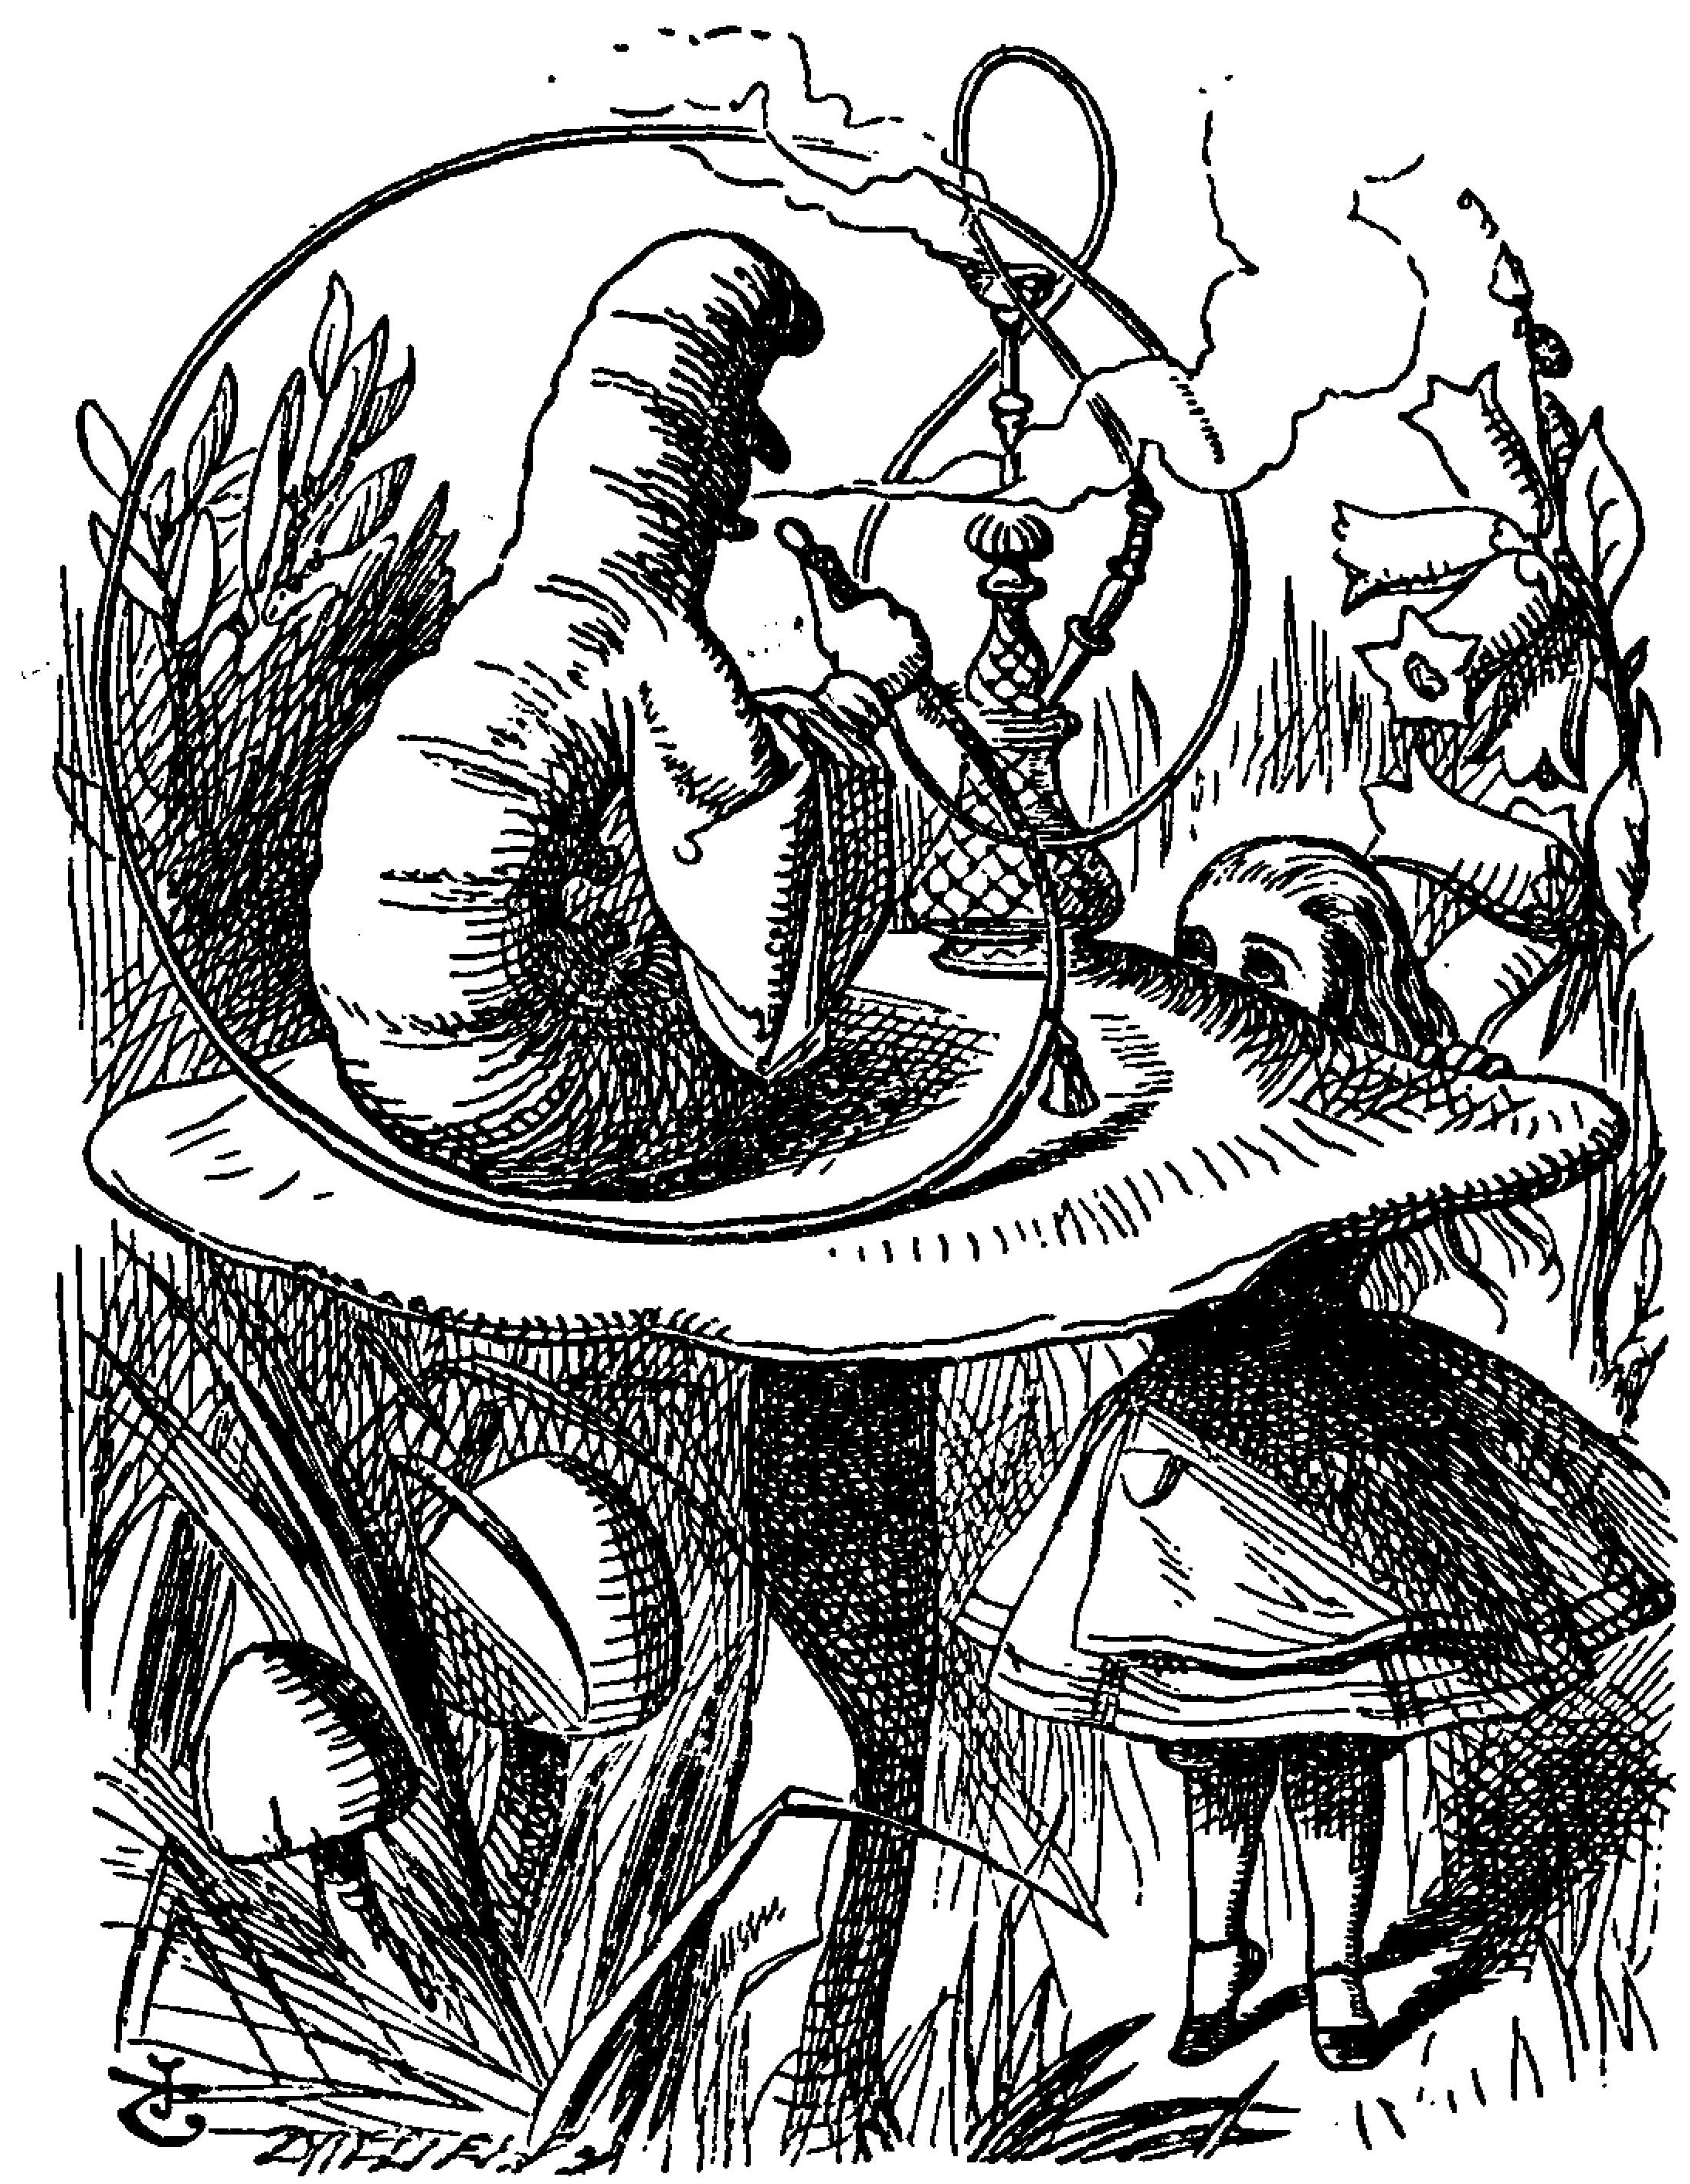
\includegraphics[width=5cm, keepaspectratio, right]{img/alice1.jpg}

\par\end{flushright}
\end{quotation}


\cleardoublepage
% \phantomsection
\addcontentsline{toc}{chapter}{Acknowledgements}

\begin{quotation}
\begin{flushright}
\textit{
To the ones who patiently supported and accompanied me during this long and winding trip.
}
\end{flushright}
\end{quotation}
\include{acknowledgements}

\cleardoublepage

\addcontentsline{toc}{chapter}{Abstract}

%\section*{Abstract}
{\setlength{\parindent}{0cm}
Massive parallel sequencing technologies are producing a vast amount of genome-wide data about cells, tissues and model organisms, useful to understand many of biological mechanisms, like protein-chromatin interactions (e.g. ChIP-Seq), DNA methylation (Methyl-Seq or BS-Seq), chromatin accessibility (e.g. Atac-Seq), global transcriptional and translational activities (e.g. RNA-Seq) and 3-D organisation of chromatin (e.g. Hi-C), giving the possibility to study same individual or experimental condition from many different points of view (transcriptomics, epigenomics, etc.) with a very high resolution. Each type of these “omic” data explains a different aspect of cellular behaviour. To give a comprehensive view of the cell regulatory mechanisms it is necessary not only to perform a single level analysis, but also to provide novel statistical and computational models for integrating different omic types within a unified study.

This thesis is focused on development of three main computational tools (\textit{ticorser}, \textit{DEScan2} and \textit{IntegrHO}), allowing data analysis and integration of multiple next generation sequencing experiments.
Additionally, a fourth tool (\textit{easyReporting}) for reproducible computational research is presented.

\textit{Ticorser} (time course RNA-seq data analyser) is a novel R package aimed to analyse time-course RNA-seq data. It offers multiple methods for differential expression data analysis and provides multiple plots useful to explore and visualize the results at each step of the analysis. Furthermore, it also provides methods for functional integration by annotating genes in pathways and GO-terms.

\textit{DEScan2} (Differential Enriched Scan 2) is a novel R package for ATAC-seq data analysis, one of the emerging techniques for investigating the chromatin accessibility. It consists in the following three-step procedure : 1) It identifies candidate regions inside each sample with a peak caller; 2) It filters out potential artefacts by aligning the candidate regions between the samples and removing those candidate regions that were not reproducible between samples 3) It produces a count matrix of regions and samples, useful for differential enrichment between multiple conditions and also for integrating this data type with other omic data, such as RNA-Seq.

\textit{IntegrHO} (Integration of High-Throughput Omics data) is a Graphical User Interface (GUI), written in R and Shiny, aimed to analyse and integrate multi-omics data types. It provides a friendly interface to the above mentioned tools, and also incorporates a wide selection of methods and other tools available in literature. This platform, through an easy point-and-click approach, enables the user to analyse and explore single omic data, such as RNA-seq, ChIP-seq and ATAC-seq and, moreover, it offers the possibility to integrate them at different levels, such as gene-peak annotation and functional annotation methods.

\textit{EasyReporting} is an R package for an automatic report creation (easyreporting), developed to address the problem of reproducibility of a computational analysis.  
Thanks to the R6 class paradigm on which is based on, it is easy to use and to extend.

Overall, this work proposes and combines several computational tools for properly analysing, visualizing, comparing, integrating and tracing different types of omics data.
}
\section*{Abstract}
{\setlength{\parindent}{0cm}
Massive parallel sequencing technologies are producing a vast amount of genome-wide data about cells, tissues and model organisms, useful to understand many of biological mechanisms, like protein-chromatin interactions (e.g. ChIP-Seq), DNA methylation (Methyl-Seq or BS-Seq), chromatin accessibility (e.g. Atac-Seq), global transcriptional and translational activities (e.g. RNA-Seq) and 3-D organisation of chromatin (e.g. Hi-C), giving the possibility to study same individual or experimental condition from many different points of view (transcriptomics, epigenomics, etc.) with a very high resolution. Each type of these “omic” data explains a different aspect of cellular behaviour. To give a comprehensive view of the cell regulatory mechanisms it is necessary not only to perform a single level analysis, but also to provide novel statistical and computational models for integrating different omic types within a unified study.

This thesis is focused on development of three main computational tools (\textit{ticorser}, \textit{DEScan2} and \textit{IntegrHO}), allowing data analysis and integration of multiple next generation sequencing experiments.
Additionally, a fourth tool (\textit{easyReporting}) for reproducible computational research is presented.

\textit{Ticorser} (time course RNA-seq data analyser) is a novel R package aimed to analyse time-course RNA-seq data. It offers multiple methods for differential expression data analysis and provides multiple plots useful to explore and visualize the results at each step of the analysis. Furthermore, it also provides methods for functional integration by annotating genes in pathways and GO-terms.

\textit{DEScan2} (Differential Enriched Scan 2) is a novel R package for ATAC-seq data analysis, one of the emerging techniques for investigating the chromatin accessibility. It consists in the following three-step procedure : 1) It identifies candidate regions inside each sample with a peak caller; 2) It filters out potential artefacts by aligning the candidate regions between the samples and removing those candidate regions that were not reproducible between samples 3) It produces a count matrix of regions and samples, useful for differential enrichment between multiple conditions and also for integrating this data type with other omic data, such as RNA-Seq.

\textit{IntegrHO} (Integration of High-Throughput Omics data) is a Graphical User Interface (GUI), written in R and Shiny, aimed to analyse and integrate multi-omics data types. It provides a friendly interface to the above mentioned tools, and also incorporates a wide selection of methods and other tools available in literature. This platform, through an easy point-and-click approach, enables the user to analyse and explore single omic data, such as RNA-seq, ChIP-seq and ATAC-seq and, moreover, it offers the possibility to integrate them at different levels, such as gene-peak annotation and functional annotation methods.

\textit{EasyReporting} is an R package for an automatic report creation (easyreporting), developed to address the problem of reproducibility of a computational analysis.  
Thanks to the R6 class paradigm on which is based on, it is easy to use and to extend.

Overall, this work proposes and combines several computational tools for properly analysing, visualizing, comparing, integrating and tracing different types of omics data.
}

\hypersetup{hidelinks} % to hide suares around links

\pagestyle{plain}\tableofcontents

\cleardoublepage{}
\pagestyle{fancy}

\include{acronym.tex}
%\include{original_articles}
\newpage
\setstretch{1.5}
%%%%%%%%%%%%%%%%%%%%%%%%%%%%%%%%%%%%%%%%%%%%%%%%%%%%%%%%%%%%%%%%%%%%

\chapter{Introduction} \label{sec:introchap}
This chapter provides all the aspects needed to understand the context of this thesis work, highlighting, moreover, which are the the proposed goals of it.
%explains some basic information useful to understand the context where this thesis work has been developed.

It starts from showing some biological basic aspects and how it is possible to study some cellular behaviours from multiple points of view, using different sequencing techniques and how to integrate them.
Showing, moreover, the importance of keeping trace of the processes involved in the information extraction and why we underlying this aspect. 


\section{Biological Background} \label{sec:bioback}
\subsection{The cell}
\label{sec:cell}
Cells are the fundamental units of every living being, which can be made up of one cell (unicellular) or more (multicellular).
Indipendently on how big and complex an organism could be, each cell always maintains its individuality and its independence, but maintaining common structural proprieties.

The internal volume is defined by the \textit{cytoplasm}, which is a liquid solution where several insoluble particles stands, such as enzimes, \textit{RNA} and metabolites.
Moreover, it is possible to distinguish multiple organelles, such as \textit{ribosomes}, the \textit{endoplasmic reticulum}, the \textit{golgi comples},\textit{lisosomes} and the \textit{nucleus} (figure \ref{fig:cell}).
In particular, this last one has a the role of contain the genome, represented by the \textit{DNA}.

\begin{figure}[h]
\centering
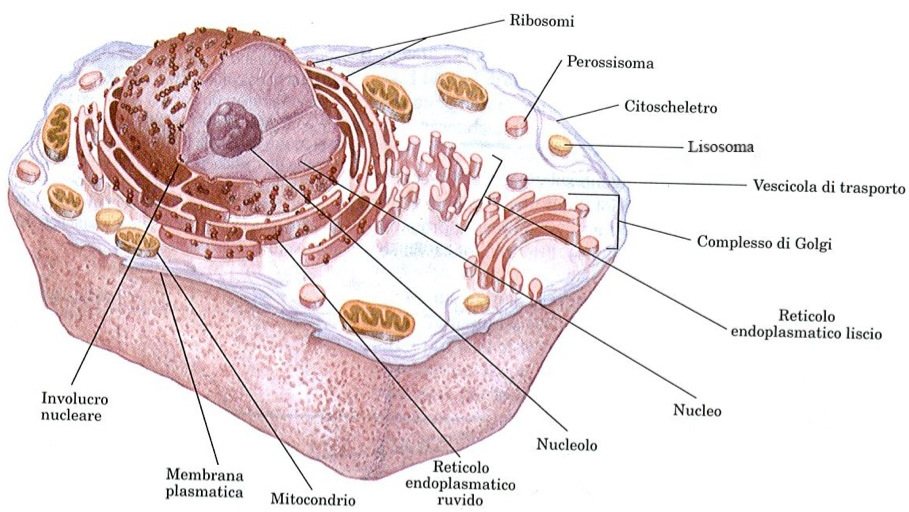
\includegraphics[width=10cm, keepaspectratio]{img/intro/cell.png}
\caption[The Cell]{Schematic representation of a cell.}
\label{fig:cell}
\end{figure}

\subsection{The DNA}
\label{sec:genica}
The \textit{DNA} was been isolated for the first time by the German doctor Friederick Miescher in 1869, while in the same decade the English biologist Charles Darwin was publishing \textit{On the Origin of the Species} and the  Augustinian friar scientist was communicating his results on the pees to the Brunn Natural History Society.

Because the substance isolated by Miescher was white, lightly acid and present only into the cells nuclei, it was been termed \textit{Nucleic Acid}.
Name modified afterwards in \gls{dna}, to distinguish is from the another one, very similar, the \gls{rna}.

These two molecules are constituted by \textit{nucleotides}, constituted by a nitrogen base, deoxyribose sugar and a phosphate group.
We distinguish two nitrogen bases, purines and pyrimidines.
Inside the \gls{dna}, we have two \textit{pyrimidines}, \textit{adenine (A)} and \textit{guanine (G)}, and two \textit{pyrimidines}, the \textit{Cytosine (C)} and the \textit{Thimine (T)}  .
Inside \gls{rna} \textit{Thymine} is substituted by the \textit{Uracil (U)}.

\begin{figure}[h]
\centering
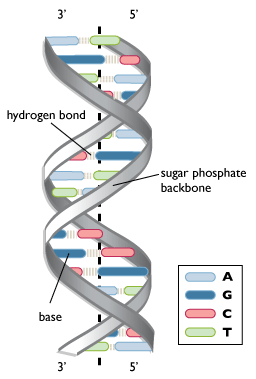
\includegraphics[width=5cm, keepaspectratio]{img/intro/dna1.png}
\caption[the \gls{dna}]{Schematic representation of double-stranded filament structure of \gls{dna}. The legend report the four nitrogen bases, Adenine, Guanine, Cytosine and Thymine.}
\label{fig:dna}
\end{figure}

\gls{dna} structure (figure \ref{fig:dna}) was discovered, in the 50's, by the American scientist James Watson, the French physicist Francis Crick and the English chemist-physicist Rosalind Franklyn.
According to their model the \gls{dna} is a double-stranded filament, where Adenines can pair only with Thymines and Guanines only with Cytosines.
The four bases constitute the alphabet for the genetic message.

\gls{dna} is folded on itself (\textit{\gls{dna} packaging}, thanks to specific "beads" called \textit{nucleosomes}, which themselves consist of eight proteins with tails, called \textit{histones}, that have the \gls{dna} wrapped on them.
This mechanism enables to store around 2 meters of chromatin inside a nucleus of a 2-10 micron diameter, when referring to Human specie.

Moreover, the \gls{dna} contains the \textit{genes}, particular sections containing relevant information for building proteins and other fundamental molecules for the cellular behavior regulation.
Each gene is localized on a precise position of a \textit{Chromosome}, which are in different number for each specie.
Each chromosome is constituted by \gls{dna} within thousands genes.

\begin{figure}[h]
\centering
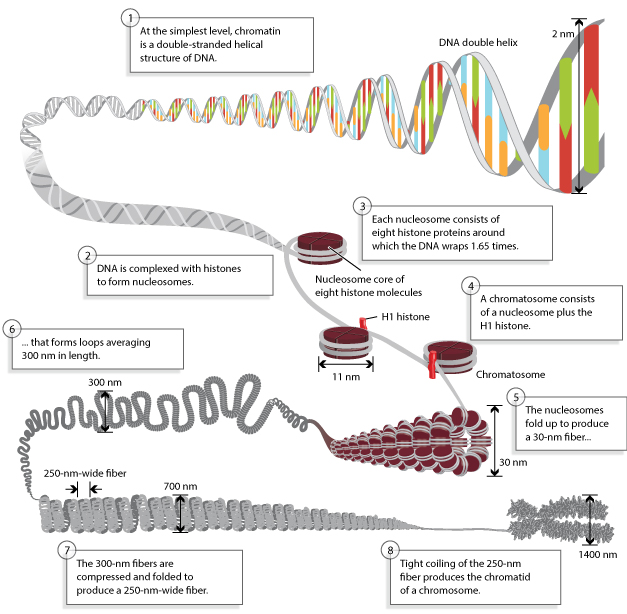
\includegraphics[width=8cm, keepaspectratio]{img/intro/dna2.jpg}
\caption[Chromosomes and \gls{dna}]{Representation of the relation between \gls{dna} and Chromosomes.
Inside the cell nucleus there are pairs of chromosome, constituted by chromatin, which fundamental unit is constituted by nucleosomes, on which the \gls{dna} is wrapped around, containing the genetic information in gene form. (image adapted from \cite{Annunziato2008})}
\label{fig:dnachromosome}
\end{figure}

Figure \ref{fig:dnachromosome} better helps  to understand the relationship between chromosomes, chromatin, nucleosomes and genes.

It is important to underlying that since some decades ago the Central Dogma of Molecular Biology was founded on the transcription - translation principle, where \gls{dna} was transcribed in \gls{rna}, which subsequently it would have been translated into protein.

Nowadays, we know that the gene transcription is regulated by several mechanisms, and moreover, the translation is not the only process fated for \gls{rna}.

Indeed, for a transcription of a gene, there are some requisites to be respected, such as the accessible of that specific part of the chromatin, or the binding of specific proteins enabling the accession to the gene region, or the histone modification processes, such as \textit{Acetylation}, \textit{Methylation}, \textit{Phosphorylation}, and others, which modifies the state of specific histones, and influencing gene expression regulation. 
  
\begin{figure}[h]
\centering
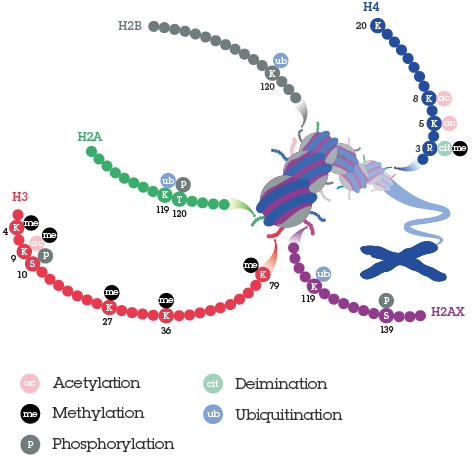
\includegraphics[width=8cm, keepaspectratio]{img/intro/hm.png}
\caption[Histon modification]{Representation of some processes involved in histone modification, influencing gene expression regulation.}
\label{fig:histmod}
\end{figure}

\section{Sequencing Techniques}\label{sec:seqs}
Several sequencing technologies have been developed during the last decades to study multiple aspects of cellular behaviour related to different experimental conditions due to drug treatments, pathologies, diseases, etc.

Starting with Sanger sequencing first and passing through Microarrays technologies then, nowadays with \gls{ngs} techniques we are able to understand many biological mechanisms, like protein-chromatin interactions (e.g. \gls{chipseq} \cite{Park2009}), DNA methylation (\gls{medipseq} or \gls{bsseq} \cite{Frommer1992}), chromatin accessibility (e.g. \gls{atacseq} \cite{Buenrostro2013}), global transcriptional and translational activities (e.g. \gls{rnaseq} \cite{Wang2009}) and 3-D organization of chromatin (e.g. \textit{Hi-C} \cite{VanBerkum2010}), giving the possibility to study same individual or experimental conditions from many different points of view (transcriptomics, epigenomics, etc.) with a very high resolution. Each type of these ''omics'' data explains a different aspect of cellular behaviour. 
To give a comprehensive view of the cell regulatory mechanisms, it is necessary not only to perform a single level analysis but also to provide novel statistical and computational models for integrating different omics types within a unified study.

The common steps valid for almost every \gls{ngs} data type starts from a library preparation (depending on the sequencing technique), an amplification of the genomic material and finally the sequencing of the samples.

The typical analysis requires several steps to achieve good quality results, regardless of the specific final aim of the investigation.
A standard analysis starts with a quality control assessment of raw sequenced fragments (reads), using software as \textit{FastQC} \cite{Andrews2010}.
After quality control assessment, in general, it is fundamental for the analysis to map the raw reads on a reference genome. 
But, depending on the sequencing technique, for the reads mapping phase we have to distinguish the aligner to use.
For \gls{dna} sequencing \textit{Bowtie} \cite{Langmead2009, Langmead2012} and \textit{BWA} \cite{Li2010, Li2009b} are the most common ones, while for \gls{bsseq} there is \textit{Bismark} \cite{Krueger2011}.

For \gls{rnaseq}, during the last years, in order to obtain higher accuracy in read mapping (alignment), several software, such as \textit{STAR} \cite{Dobin2013} and \textit{HISAT2} \cite{Kim2015}, superseded broadly used tools as \textit{TopHat2} \cite{Kim2013}.
Usually, an aligner produces \gls{bam} files\footnote{\url{http://samtools.github.io/hts-specs/SAMv1.pdf}} \cite{Li2009} where all the reads (mapped and un-mapped) are collected together with additional information, relevant for further steps of the analysis.
%Depending on the final aim of the analysis, \gls{bam} files can be further processed to delete or to split the reads. 
Usually the software used for \gls{bam} files processing is \textit{samtools} \cite{Li2009, Li2011}, available also in R programming language with \textit{rsamtools} \cite{Morgan}.
From this point on, the analysis steps dependend on the sequencing technique and from the experimental investigation.

Here, we present the basics ideas about the main approaches considered in his thesis.
%sequencing techniques addressed in this thesis work, needed to better understand the outline of next chapters.
%Please refer to the following chapters for details about each data type analysis.
\subsection{RNA-seq} \label{sec:rnaseq}
textit{RNA-Seq} \cite{Thermes2014, Wang2009, Costa2010, Ozsolak2011} is the most widely used technology to understand gene related regulatory mechanisms in response to stress conditions or drug treatments and progressions of several diseases \cite{Costa2013}.

The main aim of RNA-Seq experiment is to highlight the mainly altered processes (either up-regulated or down-regulated) when comparing two or more conditions at a specific instant in time or in subsequent time points (time-course experiment), and then identify the biological mechanisms regulating such changes.

The general idea underlying the library preparation of an RNA-Seq experiment can be viewed as the conversion of long mRNAs segments in cDNA fragments with RNA or DNA fragmentation. 
To each sequence an adapter for the sequencer is added and a short read is obtained with high-throughput sequencing technology (Figure \ref{fig:rnaseqexp}).


\begin{figure}[h]
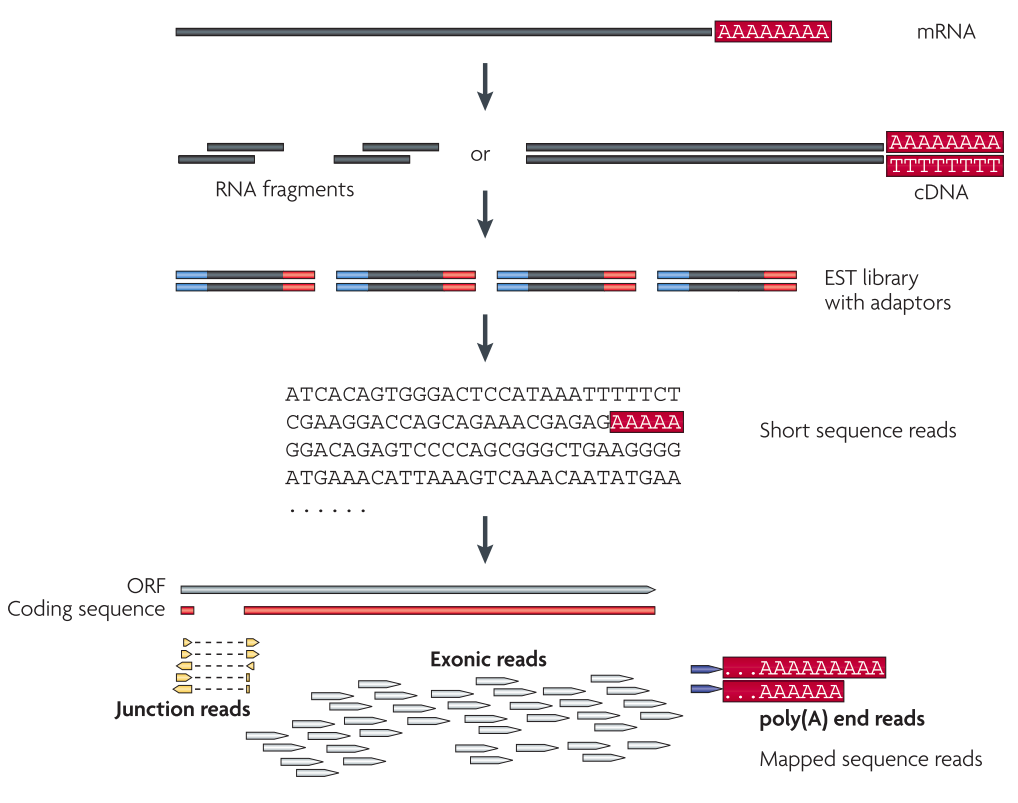
\includegraphics[width=\textwidth,height=\textheight,keepaspectratio]{img/intro/rna-seq.png}
\caption[RNA-Seq experiment]{Representation of an RNA-Seq experiment. \cite{Wang2009}}
\label{fig:rnaseqexp}
\centering
\end{figure}

In order to investigate the experiment, the so-obtained reads have to be analyzed with several tools depending on the particular question the researcher is interested in \cite{Pepke2009, Oshlack2010}.

\begin{figure}[h]
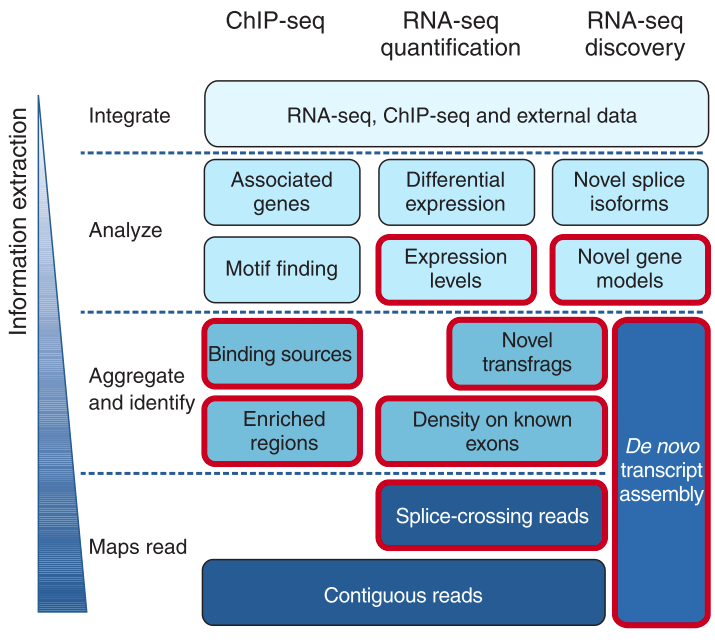
\includegraphics[width=\textwidth,height=\textheight,keepaspectratio]{img/intro/rna-seqan.png}
\caption[RNA-Seq analysis]{Representation of the possible complexity of RNA-Seq analysis. \cite{Pepke2009}}
\label{fig:rnaseqan}
\centering
\end{figure}

In particular we focused on the RNA-seq quantification in case of multiple biological conditions, due to stress, drug treatments, disease specific, etc. where a typical analysis starts from the alignment of the reads on a specie reference genome and the quantification of the mapped reads, producing a count matrix of the samples (on columns) and the genes related features (on the rows), typically identifiers depending on the annotation database used by the analyzer.
Commonly, the counts matrix needs to be filtered from low expressed features and then normalized across the samples, to reduce specific bias for each sample.
Then, it is possible to choose between several methods for the detection of differential expression of the features between the conditions (see section \ref{sec:ticorsermethods}).
Finally, the significant features can be integrated with databases of biological functionalities in order to detect the mostly influenced ones.


\subsection{ChIP-seq} \label{sec:chipseq}
As previously mentioned, epigenetic marks are fundamental aspects of the cellular biological processes. 
Indeed, their state influences not only gene accession but also the regulation of gene expression.

Some relevant aspects are \glspl{hm} and \glspl{tf}, the first ones are related to transcriptional activation/inactivation, chromosome packaging, and \gls{dna} damage/repair.
While \glspl{tf}, also named as sequence-specific \gls{dna}-binding factor, are proteins that control the transcription of genetic information by binding specific sequences of \gls{dna}.

To investigate these epigenetic aspects nowadays is mainly used the Chromatin ImmunoPrecipitation sequencing (\textit{ChIP-seq}) technique \cite{Park2009}.
This technique allows to use antibodies for selected proteins or nucleosomes, which enriches for specific \gls{dna} sequences bounded to these proteins/nucleosomes.

\begin{figure}[H]
\centering
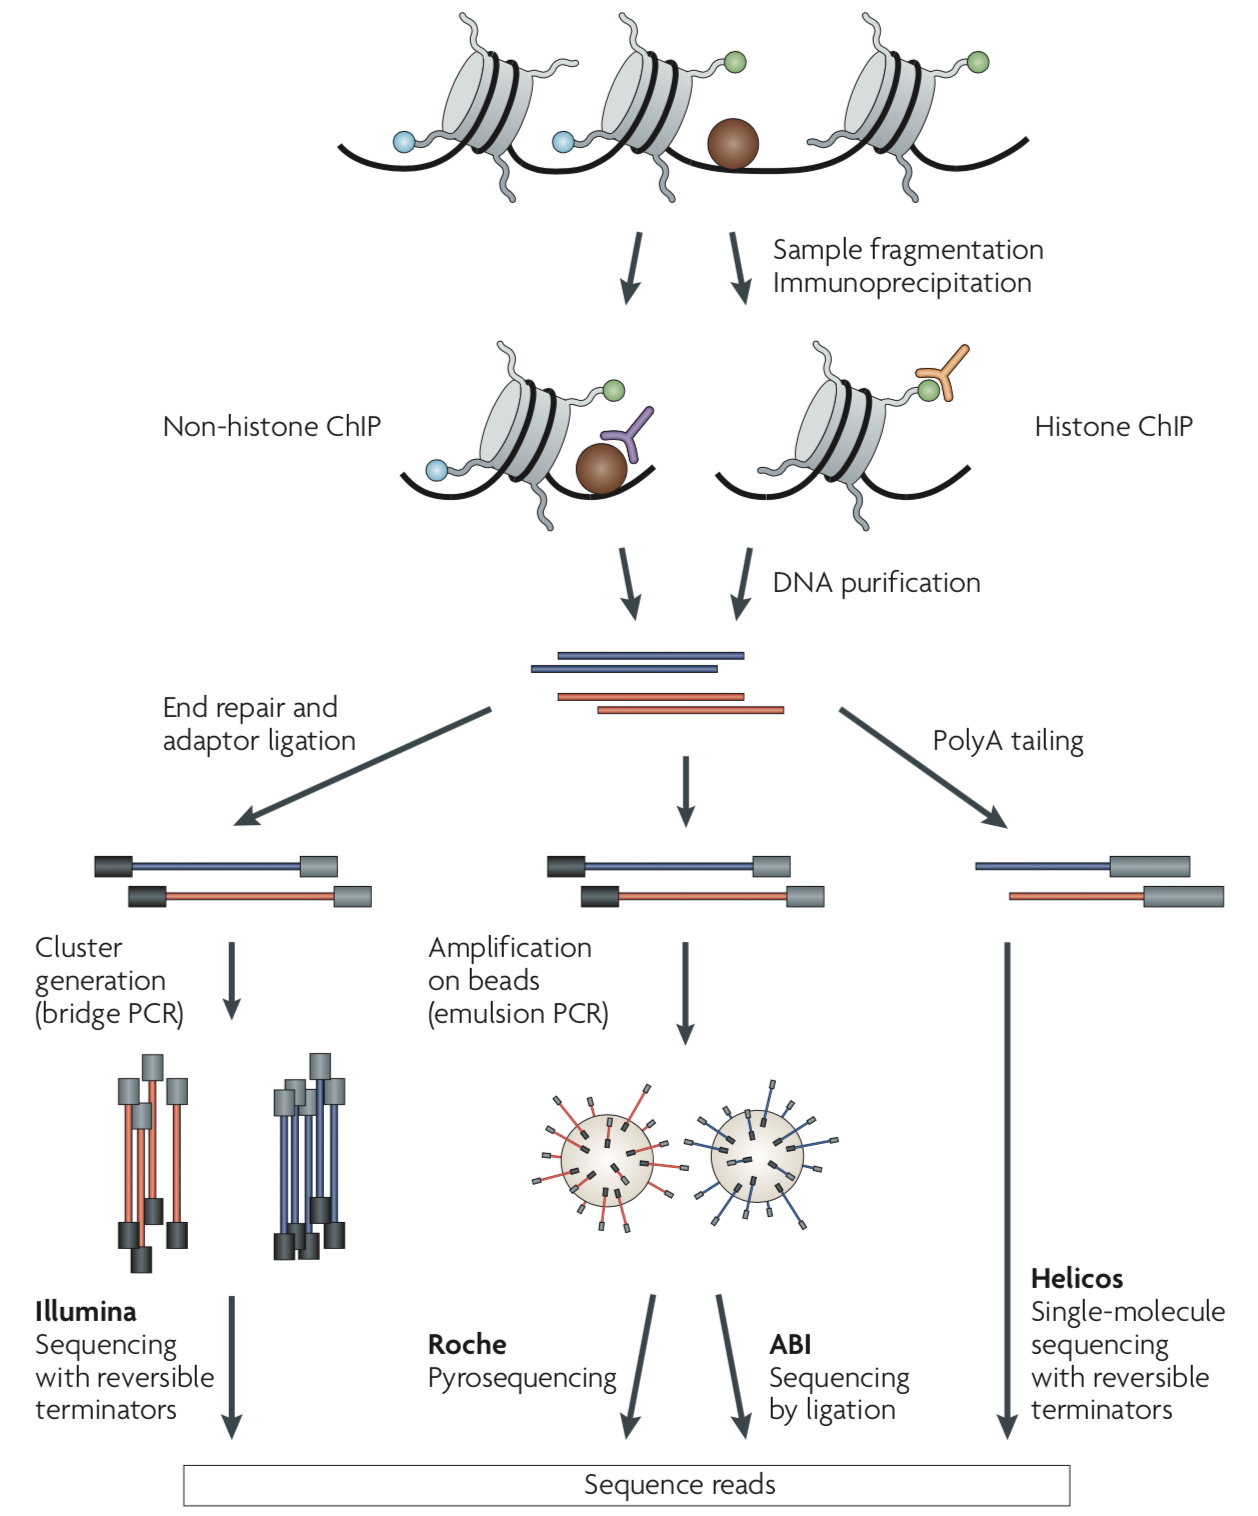
\includegraphics[width=8cm, keepaspectratio]{img/intro/chip.png}
\caption[ChIP-seq experiment]{Representation of a  ChIP-seq experiment. \cite{Park2009}}
\label{fig:chipseqexp}
\end{figure}

The library preparation consists into lock biological processes with formaldehyde and then cutting the chromatin into small fragments with sonication.
Afterwards, a specific antibody for the interested protein is used to immunoprecipitate the \gls{dna}-protein complex, in order to be purified and, after amplification, be sequenced.

When analyzing the data, it is relevant to distinguish between \gls{hm} and \gls{tf} ChIP because, even if the library preparation it's the same (it differs only for the antibody used, just because the proteins are different), the data analysis pipeline is different in methodologies used because of the different signal produced by them.
Indeed, after read mapping on a reference genome, reads need to be processed with methodologies for the protein-binding regions detection, that are typically called \textit{Peak callers}.
After the peak calling process it is possible to highlight that the \gls{tf} signals (peaks) are more narrowed respect to the ones detected for \gls{hm}, leading to develop different methodologies for investigating further aspects for each one of these \textit{ChIP-seq} signals.

\begin{figure}[H]
\centering
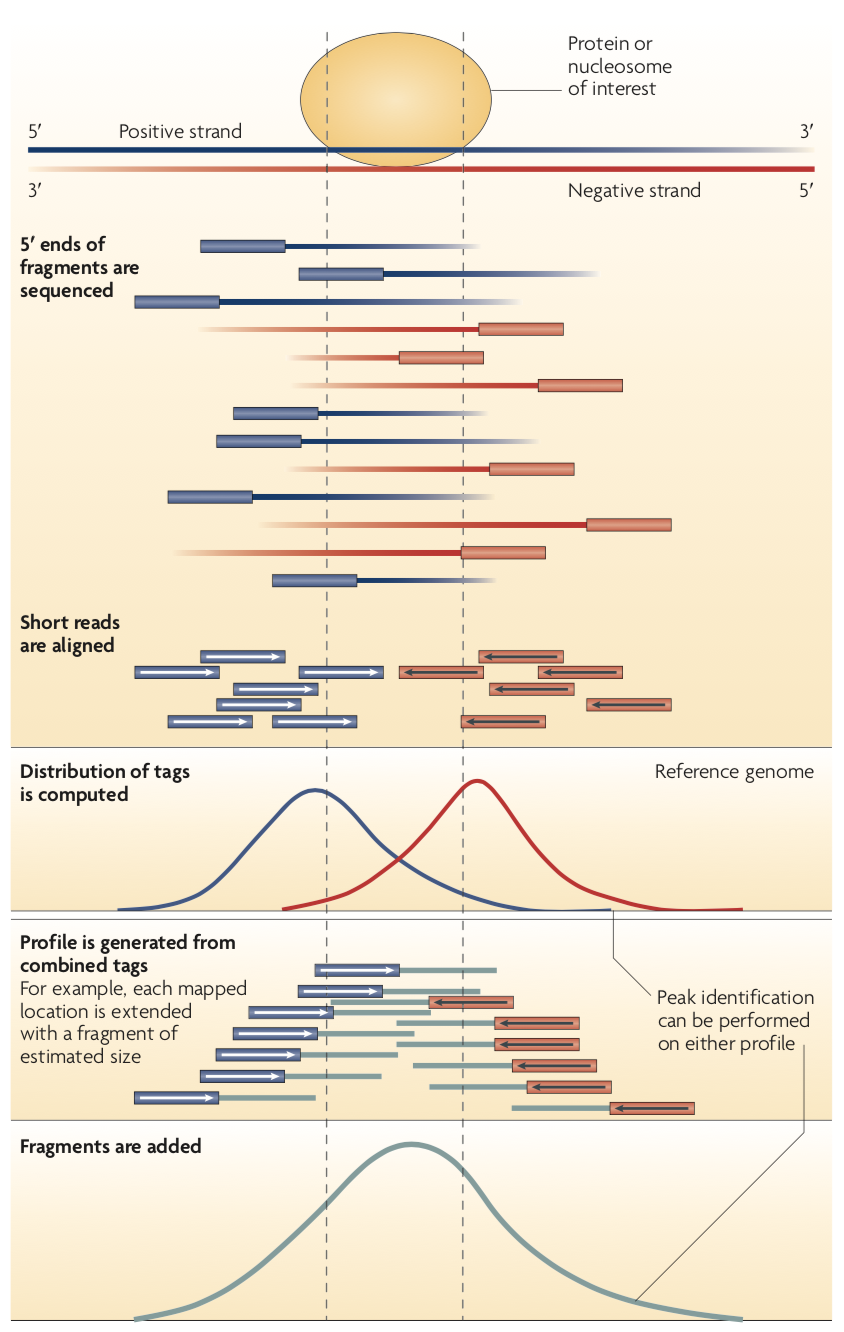
\includegraphics[width=8cm, keepaspectratio]{img/intro/peak_call.png}
\caption[ChIP-seq peak detection]{Representation of a  ChIP-seq peak calling process. \cite{Park2009}}
\label{fig:chipseqexp}
\end{figure}

Subsequently to the peak detection, several aspects can be investigated about the signal, such as the identification of motifs related to the peaks, or the genes associated with the regions detected, and, when other omics are available (e.g. RNA-seq), it is interesting to associate the expressed features (e.g. genes) and doing functional enrichment analysis. 






\subsection{ATAC-seq} \label{sec:atacseq}
The chromatin packaging of the genome plays a fundamental role in gene regulation of eukaryotic individuals.
To study this aspect of the \gls{dna} several technologies have been developed, such as \textit{FAIRE-seq} \cite{Giresi2007}, \textit{DNase-seq} \cite{Winter2013} and \textit{ATAC-seq} \cite{Buenrostro2013}, etc.

\textit{ATAC-seq} among the others is having a growing interest and diffusion in the last years, because it offers comparable results to the DNASE-seq with less biological material and less library preparation time.

\begin{figure}[h]
\centering
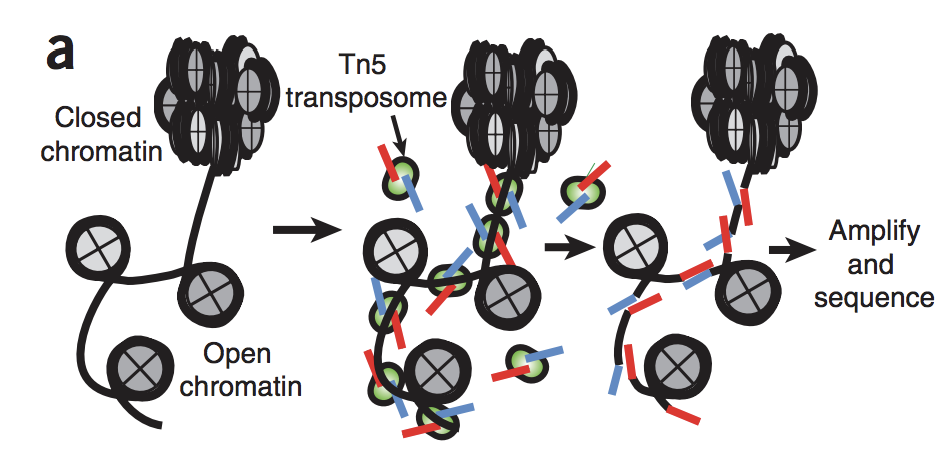
\includegraphics[width=9cm,keepaspectratio]{img/intro/atac.png}
\caption[ATAC-seq experiment]{Representation of ATAC-seq library preparation. \cite{Buenrostro2013}}
\label{fig:atacseqexp}
\end{figure}

The library preparation adopts a hyperactive Tn5 transposase, modified with adaptors for high-throughput  \gls{dna} sequencing, which is able to fragment and tag a genome simultaneously.
The technology exploit the Tn5 capability of integrating itself into active regulatory elements.

After Tn5 tagmentation, the resulting segments can be amplified and sequenced, producing sequences to map on a reference genome.
There is no standard analysis reached for the ATAC-seq analysis, but, inspired by the \textit{ChIP-seq} analysis, the resulting reads, typically, are processed with tools (peak callers) for quantifying their amplification, which produces for each detected open chromatin region a feature, the peak (generally with an associated score). 

Depending on the used tool, the peaks can be represented in different data structures, but their representation is given by the genomic coordinates; chromosome, starting and ending point of the region, the strand of the DNA on which the region lies, and additional attributes such as a score, a number of samples on which the regions has been detected, etc.

To obtain a first level of integration, the peaks can be annotated with other relevant features of the genome, such as the \gls{tss} of the genes, \gls{utr}, promoters, exons, introns, etc.  
Then, the annotated genes can be used to enrich for GO terms or pathways, reaching a second level of integration.





\section{Multi-omics Integration} \label{sec:integration}
All above-mentioned sequencing techniques are aimed to investigate only one cellular compartment at a time, but in order to obtain a more comprehensive view of the cellular behaviour, it is necessary to look at more than one omics at the same time.

\begin{figure}[H]
\centering
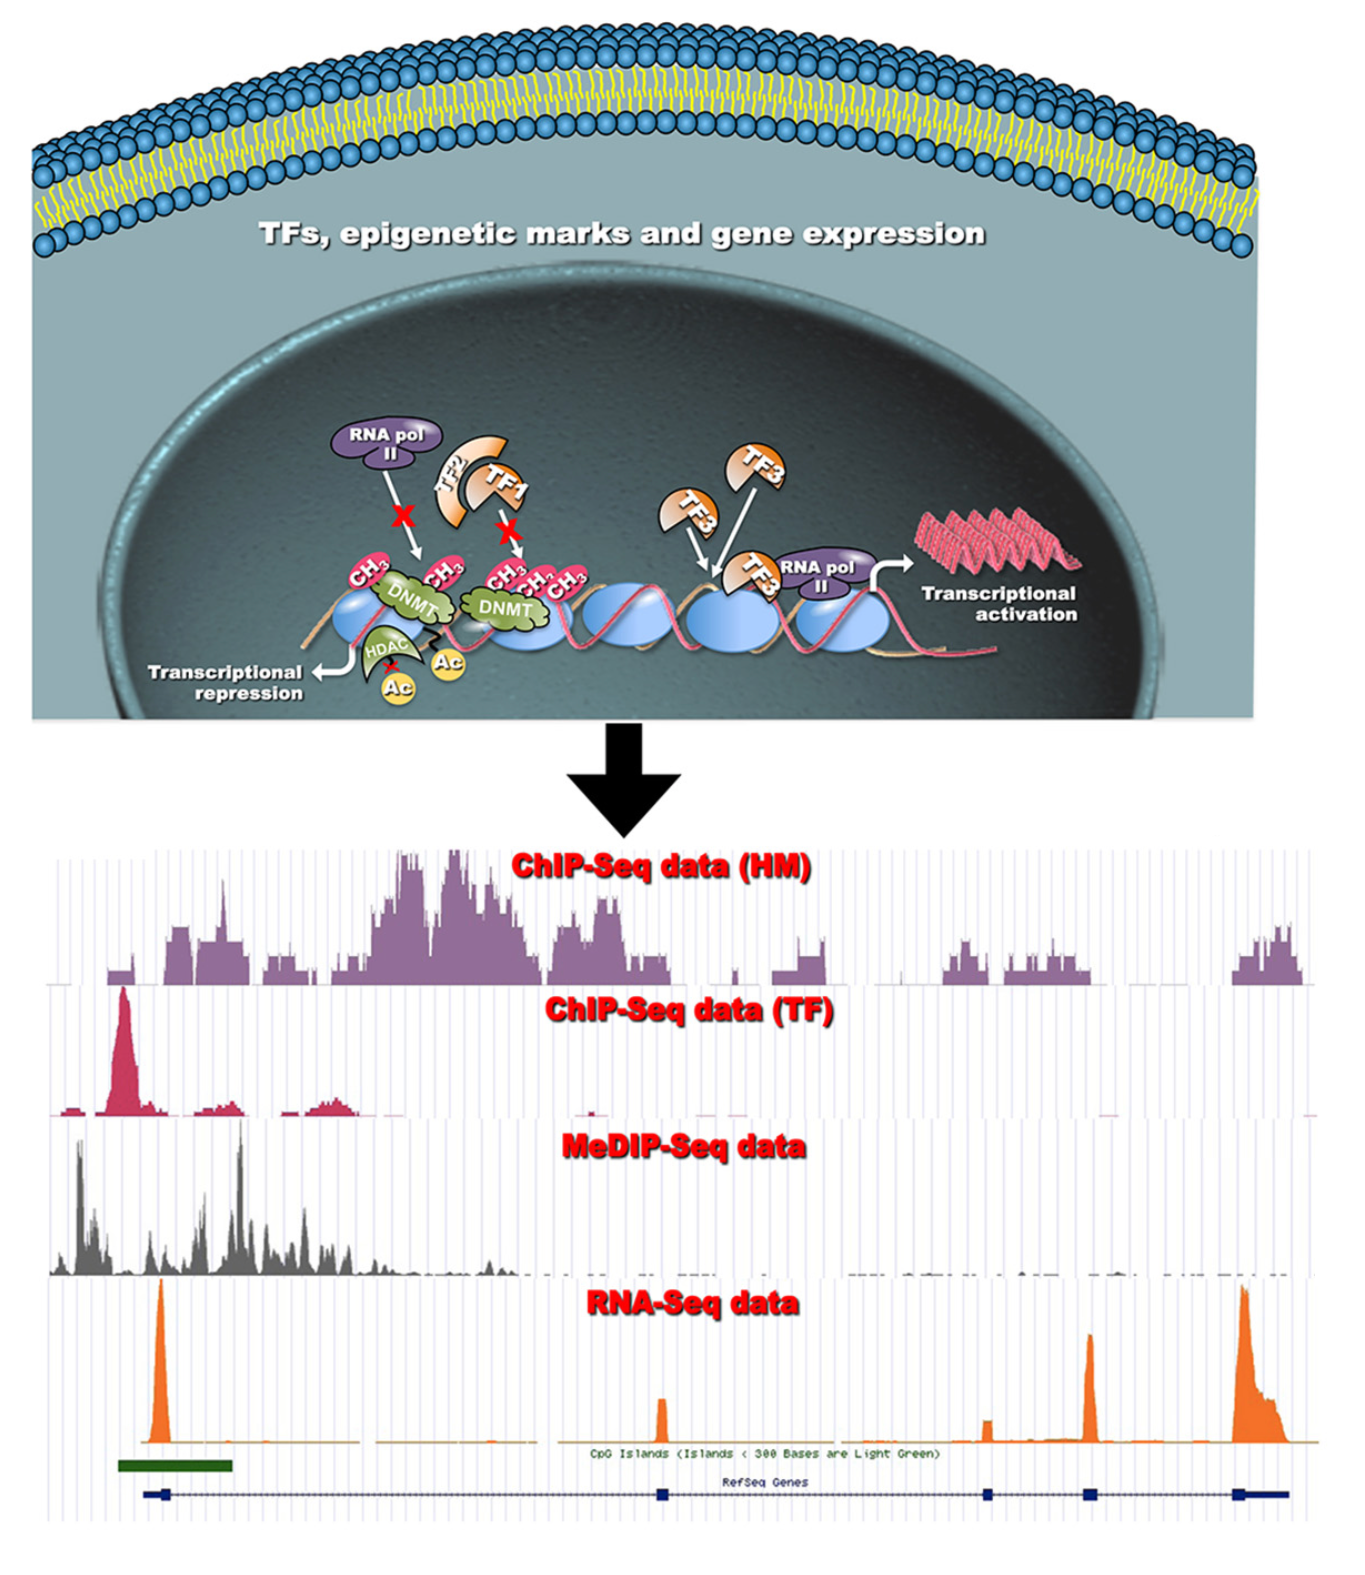
\includegraphics[width=9cm, keepaspectratio]{img/intro/multiomicsex.png}
\caption[Multi-Omics Representation]{An example of different omics coming from the same biological representation. (adapted from \cite{Angelini2014c})}
\label{fig:omics}
\end{figure}

Indeed, we can imagine each omics as a camera in a multi-view camera system pointed on a building from different points of view.
Each device takes snapshots of the building from different angles, but the information is still fragmented.
In order to reconstruct a 3D model of the building, we need to put each device snapshots together.

\begin{figure}[h]
\centering
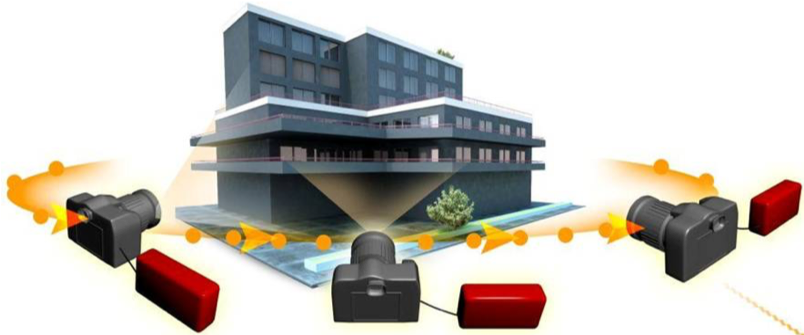
\includegraphics[width=8cm, keepaspectratio]{img/intro/cameras.png}
\caption[Integration cameras]{An illustrative exaple of a multi-view camera system pointed on a building.}
\label{fig:cameras}
\end{figure}

The same idea can be adapted to the sequencing techniques, we need to integrate the information coming from different omics in order reconstruct (and understand) how multiple mechanisms orchestrate the cellular behaviour.

Indeed, we can imagine a typical combination of epigenomics factors affecting the chromatin in order to influence the transcription of one or more genes.
An \glspl{hm} (such as \textit{Acetylation}) can have inhibited the accession to bind specific nucleosomes, because already occupied by specific \glspl{tf}, inhibiting, in such a way, the expression of those genes present in that particular portion of the chromatin (upper part of figure \ref{fig:omics}).
To investigate these processes, we can perform multiple experiments of \textit{RNA-seq} and \textit{ChIP-seq} (one for the \gls{hm} and one for the \textit{tf}) to study singularly each epigenomics factors and the gene expression (lower part of figure \ref{fig:omics}). 

As figure \ref{fig:funnell} outlines, multi-omics data integration can be made at different levels, by graphical exploration, by functional annotation, by network fusion and by dimensionality reduction.
We can distinguish two main approaches,; ''analyze each omics then integrate the results'' and ''jointly analyze each omics to improve the power''.
The first one can be done also with few samples, where each omics is analyzed standalone and then the results can be combined to obtain a common response (levels 1 and 2 of figure \ref{fig:funnell}).
The second main approach needs a high number of samples to analyze all the omics together to obtain more power in the response prediction (levels 3 and 4 of figure \ref{fig:funnell}) \cite{Rohart2017, Argelaguet2018, Jia2017, Meng2016}.

\begin{figure}[h]
\centering
\includegraphics[width=8cm, keepaspectratio]{img/intro/funnell.pdf}
\caption[Integration Funnell]{A schematic representation of multi-omic data integration levels.
}
\label{fig:funnell}
\end{figure}

More in general, integration can be performed at different levels (i.e. descriptive, exploratory, inferencial, etc.).

With graphical exploration, we can visualize data coming from different sources (e.g. \textit{RNA-seq} and \textit{ChIP-seq}) using specific tools designed at this scope, such as \textit{Genome Browser} \cite{Karolchik2011} or \gls{igv} \cite{Robinson2011, Thorvaldsdottir2013} and looking to the overlapping regions, or where expressed epigenomic markers have corrispondence with gene expression sites.

We refer to functional annotation integration when using methods combining analysis results (such as relevant lists of genes) with publicly available databases,  like the Gene Ontology\footnote{http://www.geneontology.org/} and pathway (\textit{KEGG}\footnote{https://www.genome.jp/kegg/} or \textit{Reactome}\footnote{https://reactome.org/}) based ones, to detect functional responses highly related to the experimental condition under investigation.

It is possible to integrate multiple omics data types by constructing multiple regulation networks, one for each omic analyzed, and then combine these networks with fusion techniques.
This integration aspect is used when a high number of data samples is available or when having multiple-omics data types coming from the same patients \cite{Wang2014}.

A deeper level of integration is achievable with dimensionality reduction techniques. 
Also in this case, several samples are needed to be able to obtain relevant and reliable results.
Generally speaking, these methods are able to start from multiple samples coming from different omics and to reduce their dimensionality, enabling to identify common cellular behavioural aspects \cite{Rohart2017, Argelaguet2018}.




\section{Reproducible Research} \label{sec:reprres}
The most difficult part while using a \gls{gui} is keeping track the executed functionalities during the analysis.
To face this need we equipped \gls{igro} of a \gls{rr} hidden layer (with aid of \textit{easyReporting} package) able to trace all executed code by the user.

In combination with a system of \gls{cdf}, \gls{igro} stores code chunks and the input/output data of each analysis step inside an \gls{rmd} file.

\begin{figure}
\centering
\begin{subfigure}{.5\textwidth}
  \centering
  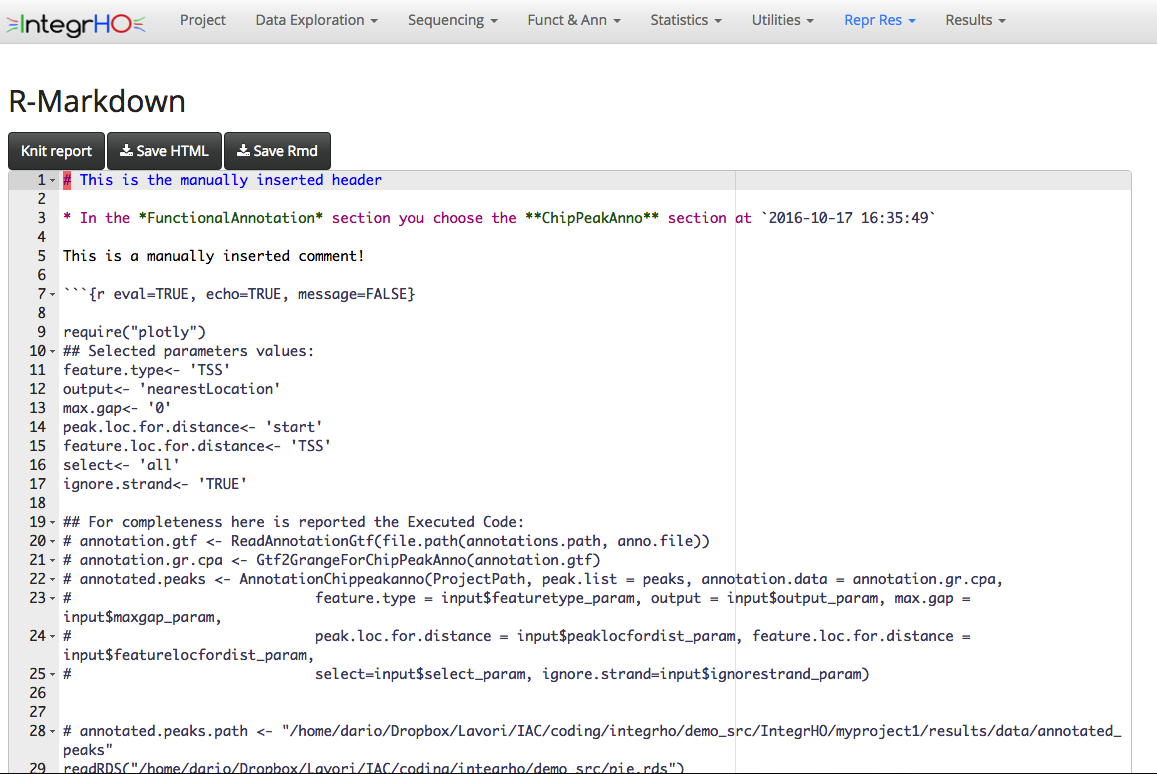
\includegraphics[width=.9\linewidth]{img/integrho/rr_1.png}
  \caption{The Interface for the editing of an auto-generated report with \gls{igro} web platform.}
  \label{fig:integrhorr1}
\end{subfigure}%
\begin{subfigure}{.5\textwidth}
  \centering
  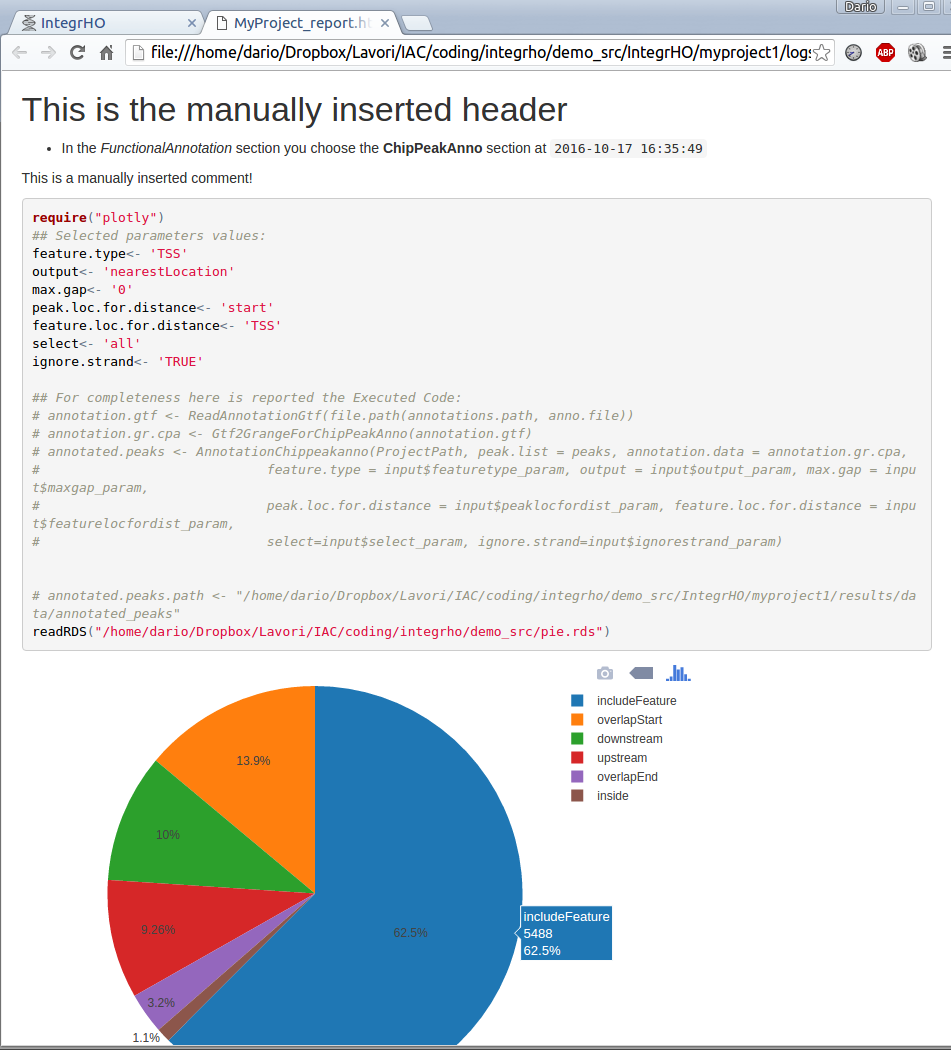
\includegraphics[width=.9\linewidth]{img/integrho/rr_2.png}
  \caption{The report compiled and enriched with manually inserted comments throught the interface showed in the (a) panel.}
  \label{fig:integrhorr2}
\end{subfigure}
\caption[IntegrHO report editing]{The reproducible research with \gls{igro}.}
\label{fig:integrhorr}
\end{figure}

The auto-produced \gls{rmd} file as it is, it's not usable to be showed to third-parties, because it needs to be enriched with natural language comments.
To account for this need, we built a specific interface enabling the user to edit the automatically produced \gls{rmd} file and to compile it on the fly (see sub-figure \ref{fig:integrhorr1}).

The enriched output report can be produced in \gls{html} (sub-figure \ref{fig:integrhorr2}) or \gls{pdf} formats, in order to be easily attached as supplementary material of a published article, facilitating the reproducibility of the analysis to third-party users.

Furthermore, thanks to the \gls{cdf} system, each code chunk is not dependent on previous ones, enabling the final user to add/remove multiple code chunks.
\section{Aim of the Work} \label{sec:reprres}
The complexity of \gls{ngs} data analysis brought the scientific community to develop multiple methodologies and tools for their analysis, reaching in some cases (such as \textit{RNA-seq}, \textit{ChIP-seq}, etc.) standard pipelines for their analysis.
However, despite such efforts, there are specific context that are much less developed and that still require attention.

Nowadays, the challenge moved on the development of statistical and computational methodologies for the information extrapolation from multiple-omics datasets, in order to produce a unified view of the biological characteristics describing the cellular behaviour.

Motivated by these aspects, we have embarked on a path that goes through the analysis of different omics to flow into multiple projects, each one with the common aim of helping the single omics analysis in order to simplify reaching the goal of integrating them in a unified view.

This thesis is focused on the development of three main computational tools (\textit{Ticorser}, \textit{DEScan2} and \textit{IntegrHO}), firstly approaching single omics data analysis and then on their integration.
Additionally, in order to face up the irreproducility problem in the scientific community, a fourth tool (\textit{easyReporting}) is presented.

\gls{tic} is a novel R package aimed to analyze time-course \textit{RNA-seq} data, which still require more attention. It offers multiple methods for differential expression data analysis and provides multiple plots useful to explore and visualize the results at each step of the analysis. Furthermore, it also provides methods for functional integration by annotating genes in pathways and GO-terms.

\gls{descan} is a novel R package for \textit{ATAC-seq} data analysis, one of the emerging techniques for investigating chromatin accessibility, for which very few methods are available. It consists in the following three-step procedure: 1) It identifies candidate regions inside each sample implementing a peak caller; 2) It filters out potential artefacts by aligning the candidate regions between the samples and removing those candidate regions that were not reproducible between samples; 3) It produces a count matrix of regions and samples, useful for differential enrichment between multiple conditions and also for integrating this data type with other omics data, such as \textit{RNA-seq}.

\gls{igro} is a \gls{gui}, written in R and Shiny, aimed to analyze and integrate multi-omics data types. 
It provides a friendly interface to the above-mentioned tools and also incorporates a wide selection of methods and other tools available in the literature. This platform, through an easy point-and-click approach, enables the user to analyse and explore single omic data, such as \textit{RNA-seq}, \textit{ChIP-seq} and \textit{ATAC-seq} and, moreover, it offers the possibility to integrate them at different levels, such as gene-peak annotation and functional annotation methods.
Trying to provide a flexible and easy-to-use tool enjoyable also by non-expert analysts, such as biologists, or beginner analysts.

Finally, since in last decades the scientific community has experienced a deep crisis known as ''irreproducible research'', this thesis presents \textit{EasyReporting}, an R package for an automatic report creation, developed to support the reproducibility of scientific research.  
Thanks to the R6 class paradigm on which is based on, it is easy to use and to extend.

Overall, this work proposes and combines several computational tools for properly analysing, visualizing, comparing, integrating and tracing different omics data types.
The results are illustrated with downloaded data from the literature or from collaboration projects.

%%%%%%%%%%%%%%%%%%%%%%%%%%%%%%%%%%%%%%%%%%%%%%%%%%%%%%%%%%%%%%%%%%%%

\chapter{Time Course RNA-seq analyzer: ticorser} \label{sec:ticorsercap}

\textbf{\textsl{few words on integration of epigenomic with transcriptomic}}

To investigate and answer epigenetic biological questions we decided to create a useful instrument for analysing epigenomic data (such as \textit{ChIP-Seq}, \textit{Atac-Seq}, \textit{Sono-Seq}).
Very often the biological questions to be answered, as for the RNA-Seq, need the comparison of two or more different biological conditions.
Starting from a set of already published \cite{Koberstein2018} scripts, we designed \textit{Differential Enriched Scan 2} (\textit{DEScan2}), a software for helping the analysis of epigenomic data.
\section{Introduction} \label{sec:ticorseintro}
In order to deeply understand and reconstruct cellular mechanisms influenced by drug treatments, pathologies or diseases, it is fundamental to look at multiple omics data types at the same time.

Previous chapters deeply described tools for multiple omics data analysis, integration and visualization using command line tools.
Even if the command line approach is pretty common inside the bioinformatics community, it is not for every scientist who is not so confident with programming languages or terminal.
When working with multiple omics data, there is an overabundance of available tools for each sequencing that can bewilder a beginner, up to the point to renounce approaching the analysis problem.

%Moreover, thanks to our previous experiences \cite{russo2015advantages} in developing \gls{gui}, we noticed a growing interest by the scientific community in using interactive software.
%This interest seems to be leaded by multiple motivations, such as the need to analyze data very fast or the lack of time in learning programming languages and terminal-line based tools.

Furthermore, even if the bioinformatics community has massively moved on the development of novel statistical and computational methods for multi-omics data integration, part of the scientific community is still anchored to the single-omics analysis side.
Even if still really helpful, it is still very common to read published papers based on single-omics data analysis without taking into account possible integrated solution with other omics data types.

Of course, it is not so simple to afford for multiple omics data experiments, but, nowadays, the internet swarms of public datasets.
In particular when looking at public biological data banks, such as \gls{geo}\footnote{\url{https://www.ncbi.nlm.nih.gov/geo/}} \cite{Services2007} or \gls{tcga}\footnote{\url{https://cancergenome.nih.gov/}} \cite{tcga2013a}, where it is possible to retrieve as many data as needed.

On the other side, if there are not so many papers publishing integrated analysis, it is also difficult for analysts to retrieve the right methodologies for the multi-omics data analysis and their visualization. 

\begin{figure}[H]
\centering
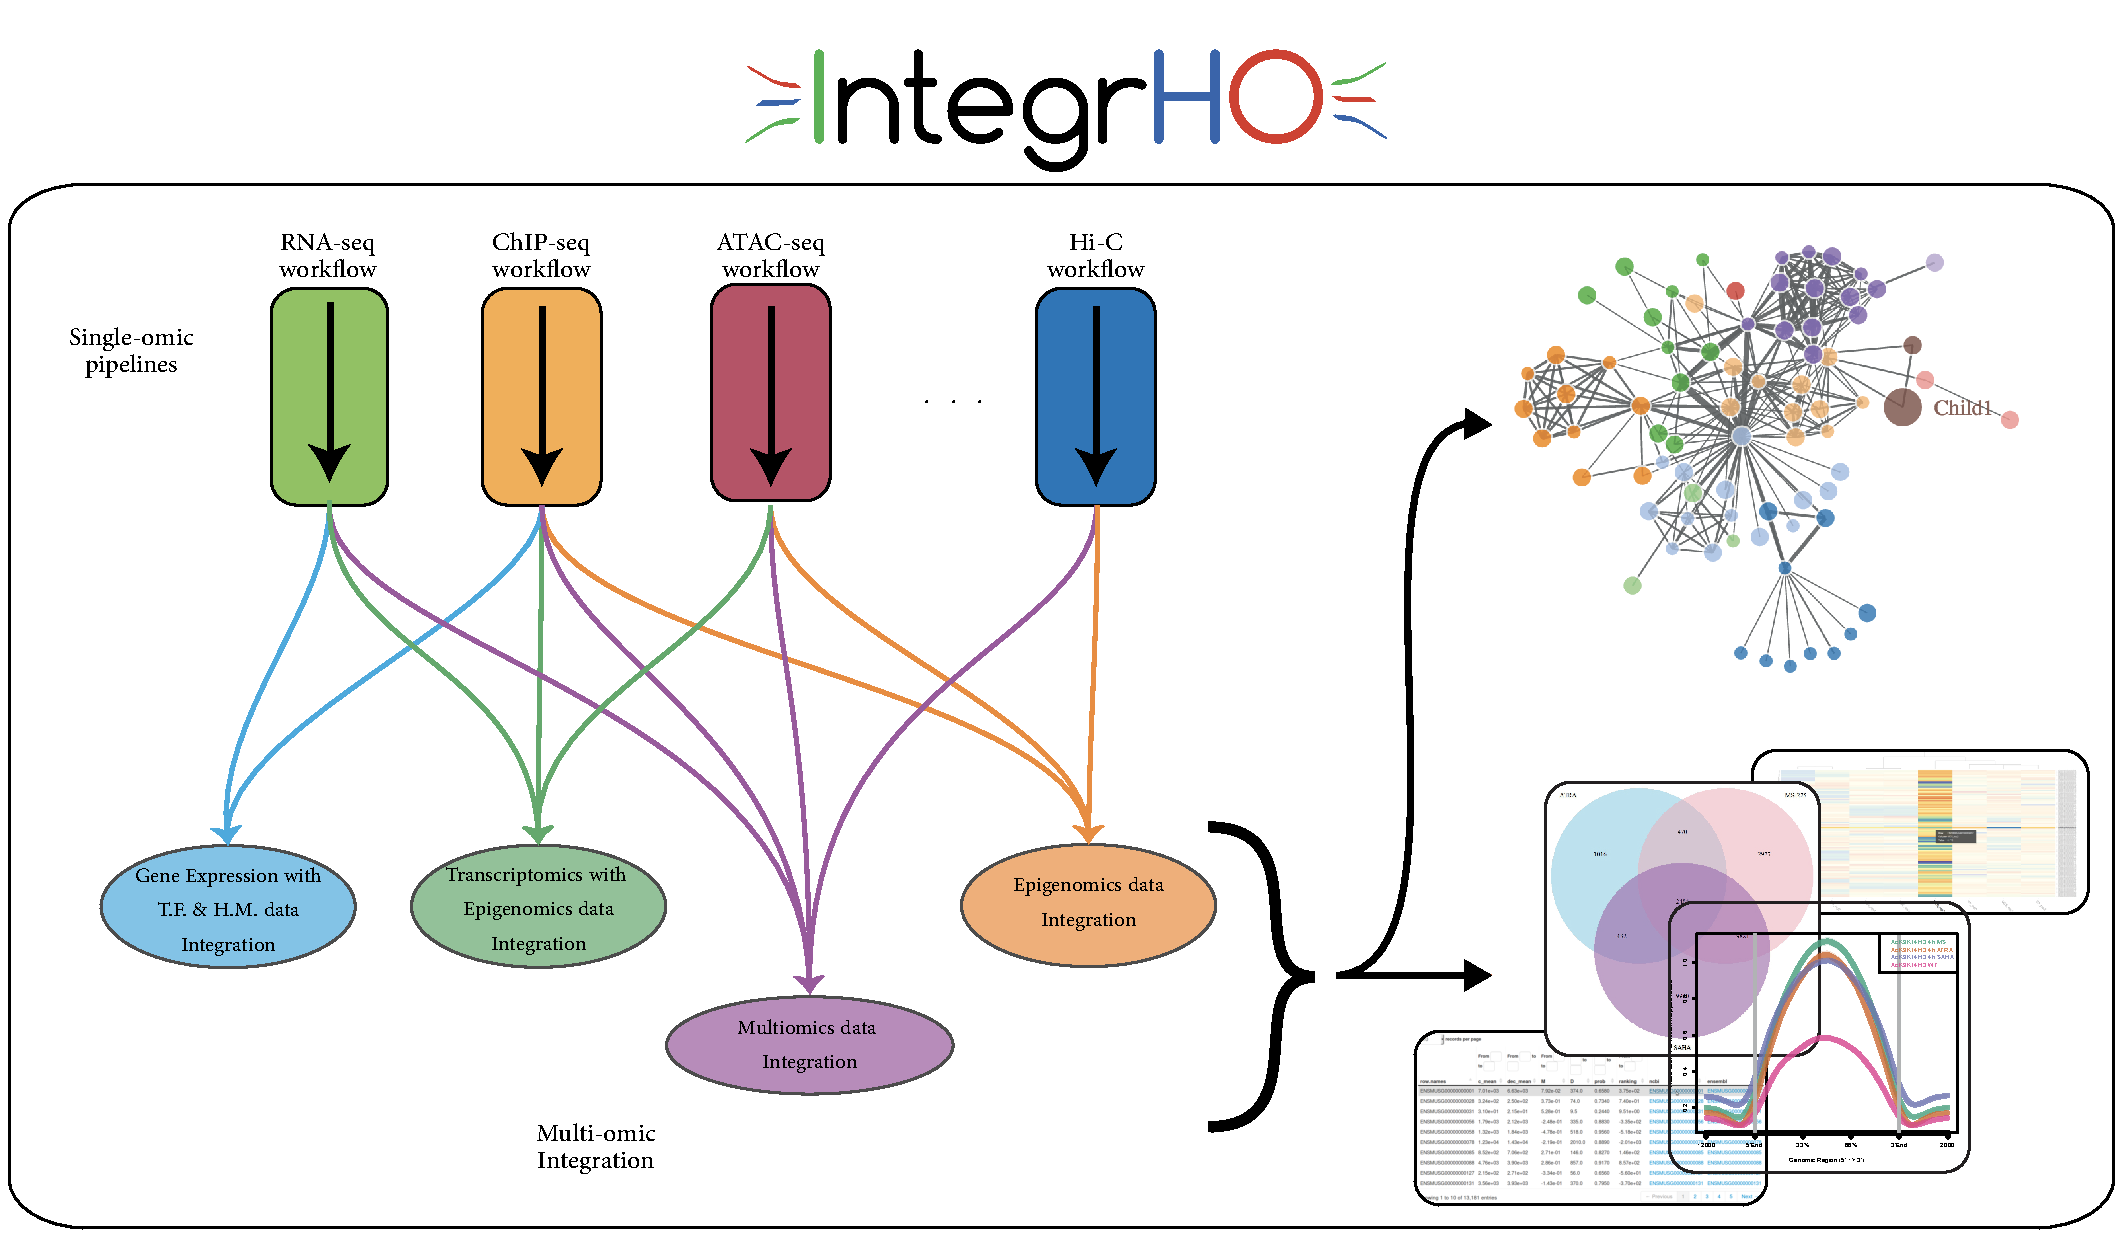
\includegraphics[width=\textwidth, keepaspectratio]{img/integrho/integrho_scheme.pdf}
\caption[\gls{igro} representation]{A schematical representation of \gls{igro} underlying idea.
Single-omics analysis methods are proposed in order to facilitate their multiple integration.
This integration can lead to produce graphical results, in case of low dimension datasets, or to more sophisticated integration model such as regulation networks, in case of high-dimension datasets.}
\label{fig:integrhoidea}
\end{figure}

Based on these considerations and in order to promote the multi-omics data integration, we decided to provide the scientific community of a novel easy-to-use instrument which not only gives the possibility to analyze single-omics data types but also guides the user through multiple ways of integrating multi-omics data types (figure \ref{fig:integrhoidea} gives an underlying idea of \gls{igro}).





%Several interface-based tools \cite{Poplawski2016} have been proposed during last years but too often they are oriented to analyze singular-omics or when designed for multi-omics, they are pipeline oriented. 

%In this chapter we introduce \gls{igro}, our web-based platform for multi-omics data analysis and integration,  in a \gls{rr} spirit.



\section{Methods} \label{sec:ticorseintromethods}
\gls{tic} is a tool fully devoted to the \gls{tc} RNA-Seq data offering features to inspect data, to normalize them, to capture differential expression of genes at static time point and overall time points, supporting different experimental designs.

Moreover, it's possible to compare the results of different analysis and to investigate the most influenced biological functions (i.e. Gene Ontology terms and Pathways). 

Overall, \gls{tic} offers the possibility to analyze data using different R packages, to compare the results in order to choose the best combination of tools for the user specific problem. Therefore, \gls{tic} offers a vast amount of exploratory and diagnostic interactive plots to explore data not just at pre-processing but also during the post-processing phase. 

\gls{tic} automatically implements a set of Reproducible Research functionalities to trace all the analysis steps selected by the user, generating a final report with both executed analysis code chunks and their produced results. Furthermore, \gls{tic} has been provided also of a caching system providing, for each analysis step, a caching database file within all the input and output processed data, useful, not only to speed up computations, but also to share data and results through the Internet.

It gives the possibility to analyse time course RNA-Seq data starting from \textit{BAM} files.
It enables RNA expression quantification with \lstinline!featureCounts! method producing a count matrix useful for \glspl{deg} detection.

We gave particular attention to the normalization phase, giving the possibliity not only to use several traditional normalizations methods, but also the possiblity to remove batch effect.


\begin{figure}[h]
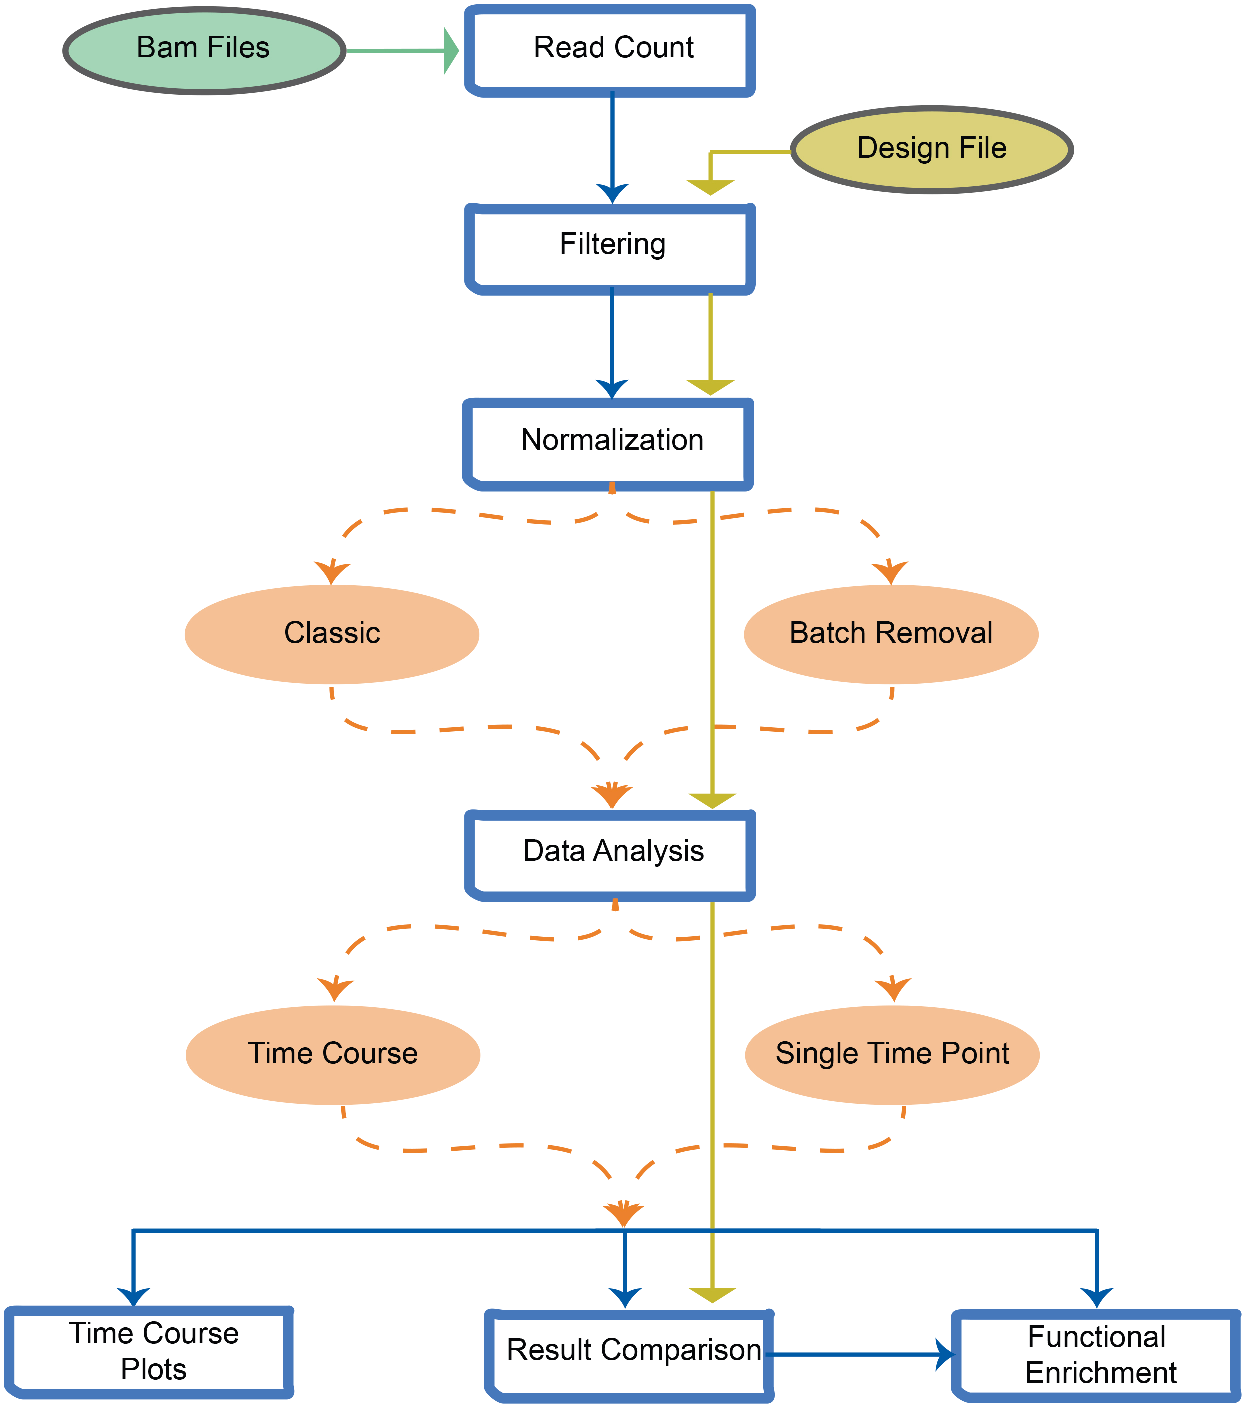
\includegraphics[width=\textwidth,height=\textheight,keepaspectratio]{img/ticorser/main_flow.pdf}
\caption[ticorser mainflow]{Main flow of ticorser R package.}
\label{fig:ticorserflow}
\centering
\end{figure}

\gls{tic} offers four different ways for analyzing time course RNA-Seq data.

Moreover, it offers three different ways for analyzing different biological conditions in a single time point.
\subsection{Filtering low counts} \label{sec:ticorserfiltering}
Low expressed genes in \textit{RNA-seq} data, always affect the detection of \glspl{deg} \cite{Sha2015} influencing final results.

In order to address this task, \gls{tic} offers multiple statistical methods for low expressed genes filtering. 
The \lstinline!filterLowCounts! method is partially based on the \lstinline!filtered.data!  function of \textit{NOISeq} R/Bioconductor package \cite{Tarazona2011, Tarazona2015}. 
The method gives the possibility to apply four different filtering methods, the \gls{cpm}, the \textit{proportion} and the \textit{Wilcoxon} tests and an our-defined method named \textit{quantile}.

The \gls{cpm} filters out all those genes with a mean expression between the samples lesser than the \lstinline!cpm! parameter threshold and, at the same time, a \gls{cov} higher that the \lstinline!cv.percentage! parameter in all the samples.

The \textit{proportion} test performs the homonym test on the counts, filtering out all those features with a relative expression equal to $cpm/10^6$.

The \textit{Wilcoxon} test filters out all those genes with a median equal to $0$.

Finally, the \textit{quantile} method enables to filter out all those genes which express the counts mean between all the samples higher than the \lstinline!quantile.threshold! argument (default is $99\%$).
\subsection{Data Normalization} \label{sec:ticorsernormalization}
Normalization is a fundamental aspect in \textit{RNA-seq} data analysis, especially when a comparison between different biological conditions is aimed to highlight the major differences.

For this reason \gls{tic} is particularly focused on this aspect. Indeed, through the \lstinline!normalizeData! function \gls{tic} provides five different normalization methods without taking care of particular additional information, except for the normalization method.
Thanks to the design matrix based system, the method allows to automatically subset the data only to the relevant factors the user want to normalize.

The function offers the possibility to normalize the data with \textit{Full quantile}, \textit{Upper quartile} and \textit{Trimmed Mean of M-values}, setting the \lstinline!norm.type! parameter to \textit{fqua}, \textit{uqua} or \textit{tmm}.

Moreover, it is possible to apply a batch effect removal normalization method, as described in \textit{RUVSeq} R/Bioconductor package \cite{Risso2014h}, focusin the attention on \textit{RUVg} and \textit{RUVs} normalization methods.

The first one, \textit{RUVg}, can be selected by setting the \lstinline!norm.type! parameter to \textit{ruvg}, which requires a list of negative controls genes with \lstinline!negative.controls! parameter.
If it's not already available from previous studies, this list can be produced by executing a first \textit{differential expression} analysis, and taking the less significative genes.

In order to facilitate this process we developed a method for creating the negative control genes list from a differential enrichment result matrix.
The function \lstinline!estimateNegativeControlGenesForRUV! takes as input the \lstinline!de.genes! and the \lstinline!counts.dataset! dataframes to extrapolate the less significative genes and to redistribute them in bins representing the mean value of the genes.
By selecting one or two genes per each bin our method is able to produce a list of negative control genes which have equal distribution for each gene counts trend.

Finally, the \lstinline!normalizeData! function offers the possibility to remove batch effects with \textit{RUVs} normalization, which is more robust to the negative controls, giving better results when their estimation is approximated.
This method taking care of creating the group samples and also the negative controls list, in case this one is \lstinline!NULL!.

\subsection{Differential Expression} \label{sec:ticorsermethods}
\gls{tic} offers four different ways for analyzing time course RNA-Seq data.

Depending on the biological question under investigation we designed three different ways of interrogate the data in a time-course experiment.

Moreover, \gls{tic} offers three different ways for analyzing different biological conditions in a single time point.

To do so, we took advantage of some of the mostly used and well-performing \cite{Costa-Silva2017} R/Bioconductor packages, \textit{DESeq2}\cite{Love2014};\textit{MASigPro}\cite{Nueda2014}; \textit{edgeR}\cite{Robinson2009}; \textit{NOISeq}\cite{Tarazona2012}.

In the following sections we firstly present the Time-Course methods and then the methods for single time point gene differentiation.

\subsubsection{Time-Course DE Method 1 - \textit{LRT-TC}}
The first method (\textit{LRT-TC}) uses a \gls{lrt} to compare two different models in order to extract all those \glspl{deg} that invert their expression expression between the conditions across all the time points.

Exploiting the \gls{lrt}, as implemented in \textit{DESeq2} R/Biocnductor package, we compare two different formulas.
The first one defines the \textit{full} model where we put together the timepoints, the conditions and an interaction term between these two variables, while the second one is a reduced model where the interaction term is removed:

In so doing we are able to catch all the genes inverting their expression across the conditions along the time-course experiment. 

\[LRT \sim \frac{times+conditions+times:conditions}{times+conditions}\]


\subsubsection{Time-Course DE Method 2 - \textit{LRT-T}}
The underlying idea of the second method is the same of the first one, where the difference, here, is to remove from the \textit{reduced} formula, not only the interaction term, but also the \textit{conditions} variable.
In such a way we are able to extract all those \glspl{deg} that have different expression profiles between the conditions across all the time points.

The first formula here defines the same \textit{full} model of the first method, while the second one is the reduced model where only the times appear:

\[LRT \sim \frac{times+conditions+times:conditions}{times}\]


\subsubsection{Time-Course DE Method 3 - \textit{LRT\_NOInteraction}}
Using always the \textit{DESeq2} \gls{lrt} we defined a third method for the 
identification of \glspl{deg} that have different expression between the conditions across all the time points, but that maintain the same profile in both conditions.

Here the \textit{full} model defines the time points and the conditions variables without taking into account the interaction term, while the second the \textit{reduced} model presents only the time point variable:

\[LRT \sim \frac{times+conditions}{times}\]


%\subsubsection{Time-Course DE Method 4 - \textit{nextMASigPro}}
%
%The fourth method takes advantage of the \gls{glm} with Negative Binomial distribution as defined in the \textit{maSigPro} R/Bioconductor package.
%This method, unlike the previous ones, allows to detect all the \glspl{deg} showing any kind of differences between the conditions across all the time points.
%Indeed, as suggested by the \textit{maSigPro} authors is a good norm to cluster the genes to better understand which is their singular behaviour.


\subsubsection{Single DE Methods}

To account for fixed time point experiment we implemented functionalities for helping also the exporation of this aspect, using three different methodologies.
 
%Our package offers a way to analyze the differences between the conditions at single time point, offering three different methodologies.

By using the \lstinline!differentiateConditions! function, it is possible to choose between the \textit{edgeR}, \textit{DESeq2}, \textit{NOISeq} and \textit{NOISeqBio}.

In case of \textit{edgeR} we decided to use the \textit{Quasi-Likelihood} method for the differential expression.
While when using \textit{DESeq2} for this specific case we choose the \textit{Wald} test, as suggested by the authors.

The \textit{NOISeq} package offers the possibility to discriminate between \textit{biological} and \textit{technical} replicates, computing a posterior probability in both cases. 





\subsection{Data Visualization} \label{sec:ticorserplots}
While analyzing RNA-Seq data, it is almost mandatory to explore data during each step of the analysis, in order to understand which is the best method to apply for the next step and to be sure that the analyzed data are trusty.

In order to help to analyze RNA-Seq data, we implemented in \gls{tic} several useful graphics at each analysis step.

Each of them, except when otherwise declared, enables to convert the plot in an interactive \textit{HTML} plot, useful to inspect additional attributes.

\subsubsection{Exploration Plots on Counts}
For exploring counts data we implemented two very common plots, the \textit{Boxplot} and the \gls{pca}.

The \textit{boxplot} is a graphical representation of the distribution of the samples, in our case we decided to plot a \textit{boxplot} for each sample and to colour them according to the time-point they belonging to.
It is a box divided in two parts, with an outgoing segment from each side. 
The upper and lower part of the box represent the first and third quartile, while in the middle is represented the median.
The upper and lower part of the segments represent the minimum and maximum values of the sample distribution.


\begin{figure}[H]
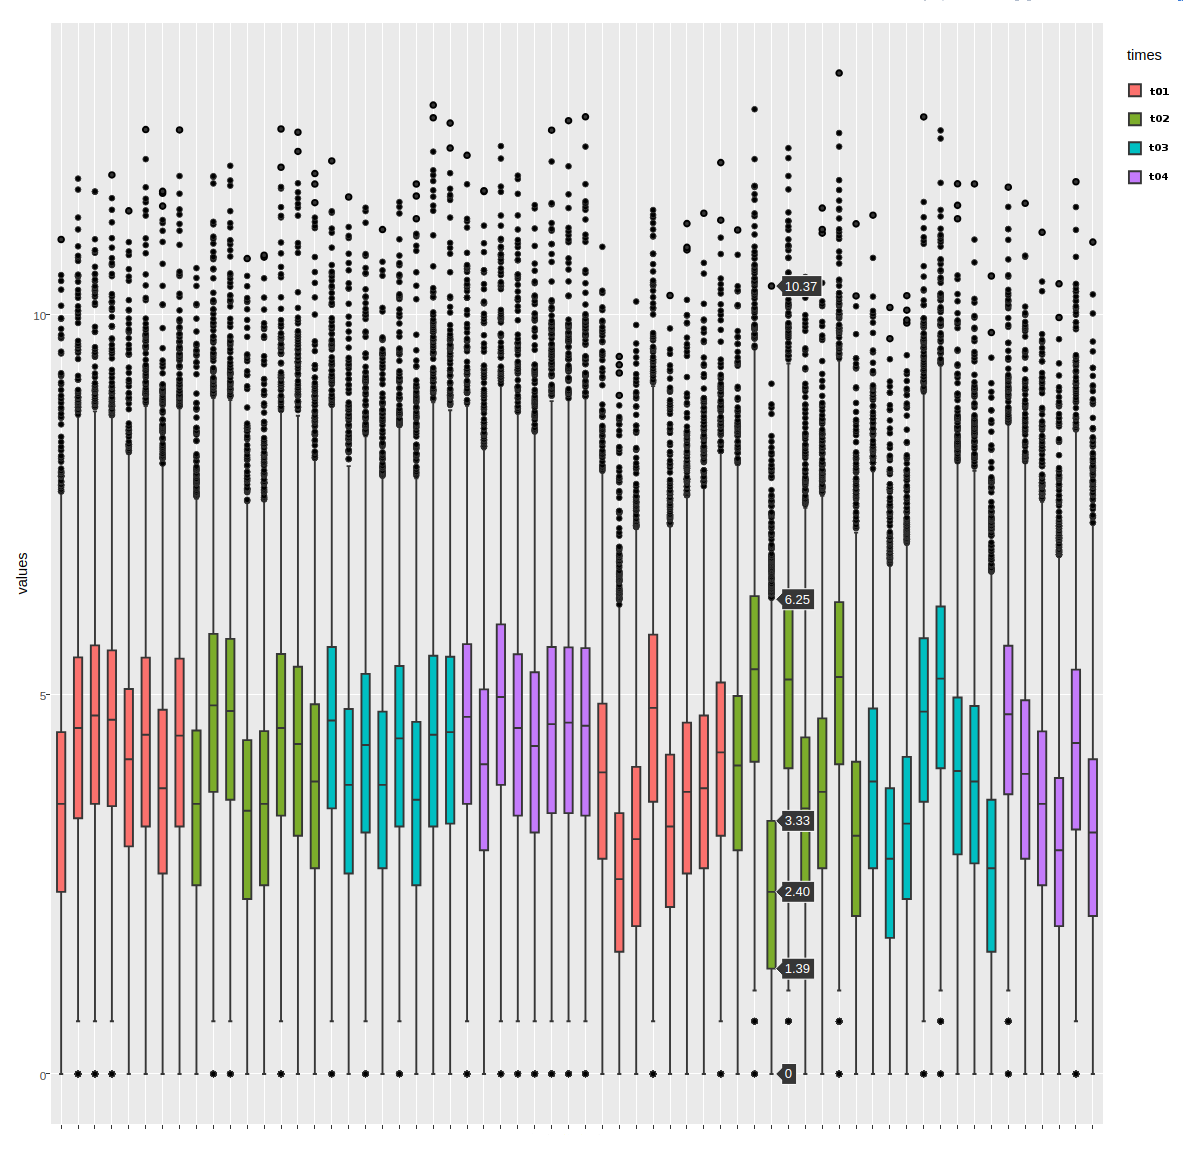
\includegraphics[width=\textwidth,height=\textheight,keepaspectratio]{img/ticorser/boxplot_example.png}
\caption[ticorser boxplot]{An example of interactive boxplot made with \gls{tic} package. Each boxplot represents a specific sample, while each colour represents a specific time point. When passing the mouse over a boxplot it shows additional information about its quartiles.}
\label{fig:ticorserboxplot}
\centering
\end{figure}
 

Due to the very high dimensionality of RNA-Seq data, it is widely considered common sense to apply \gls{pca} dimensionality reduction technique, which allows to visualize the data limiting their representation to 2 or 3 dimensions.
There are several packages allowing to apply a \gls{pca} transformation, but we choose to implement it in the \lstinline!plotPCA! function, by using the \lstinline!prcomp! from the \textit{stats} package.
The user needs just to give the \lstinline!counts.data.frame! and the \lstinline!design.data.frame! by specifying the column name where to find the samples groups.
In such a way, the function will compute and plot the \gls{pca}, coloring the samples according to the groups identified in the chosen column.
Moreover, by setting to \lstinline!TRUE! the \lstinline!ellipses! argument, the function will plot also the ellipses surrounding each sample group.

\begin{figure}[H]
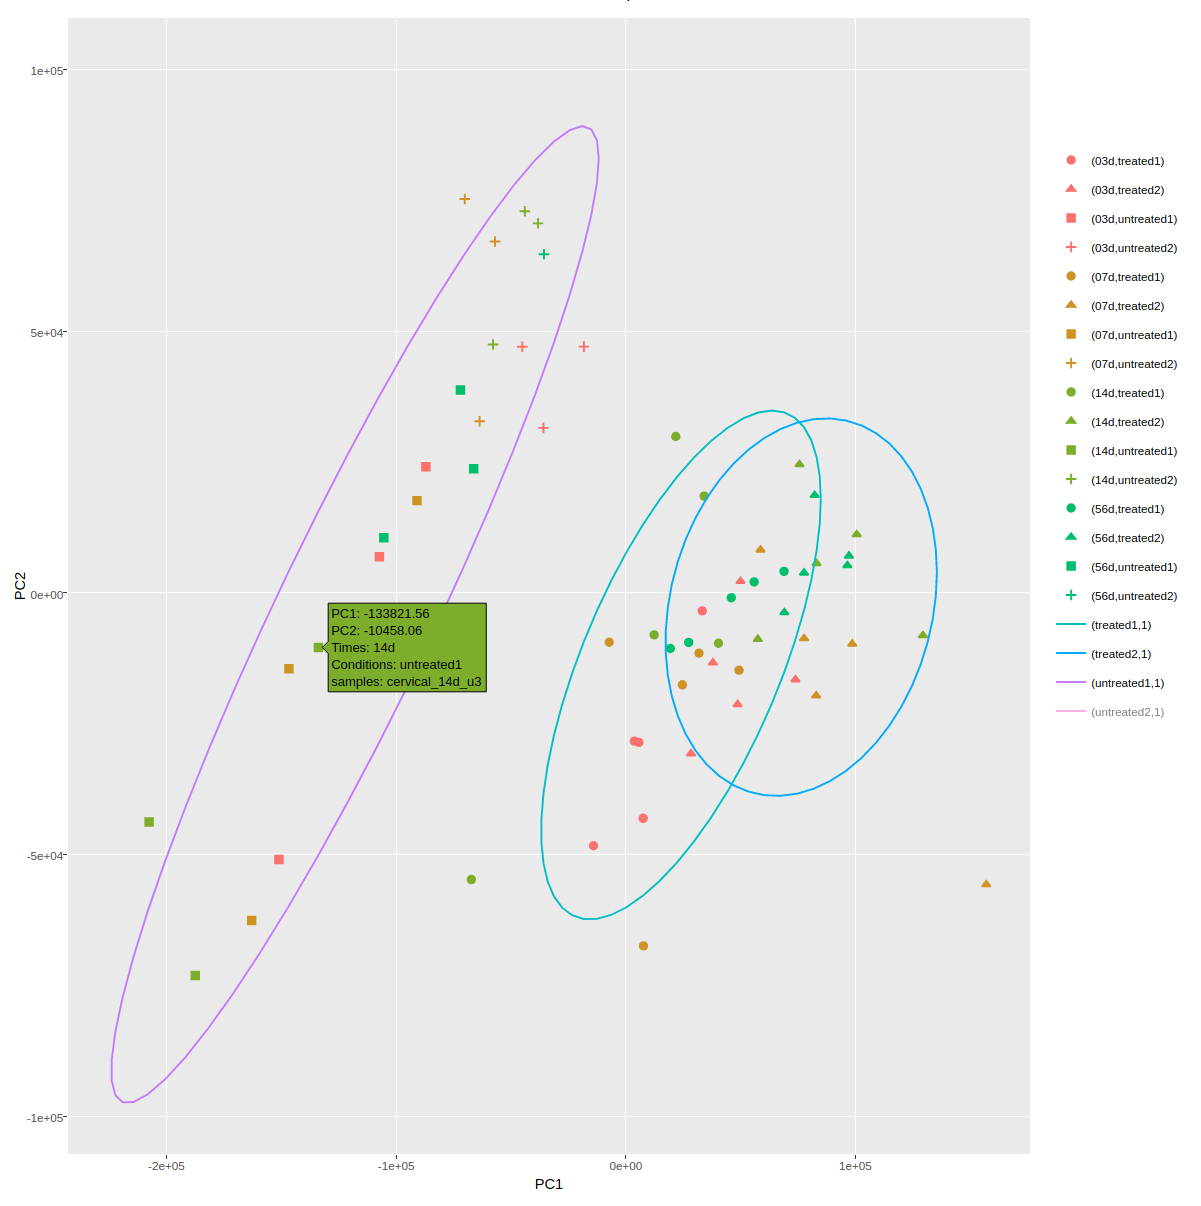
\includegraphics[width=\textwidth,height=\textheight,keepaspectratio]{img/ticorser/pca_example.png}
\caption[ticorser pca]{An example of interactive \gls{pca} made with \gls{tic} package. Each dot represents a specific sample, while each colour represents a time point, each simbol represents a biological condition group. When passing the mouse over a dot it shows additional information about the selected sample, while from the legend it's possible to show/hide groups or ellipses.}
\label{fig:ticorserpca}
\centering
\end{figure}

\subsubsection{DE Results Plots}
In order to inspect the results producted by DE methods, we implemented two kind of very common plots, the \textit{VolcanoPlot} and the \textit{MAPlot}.

Both our implementations takes as input a DE results data frame automatically recognizing which method produced it.
Moreover, it gives the possiblity to add a list of positive control genes, in order to annotate them on the volcano plot with a third colour.

The volcano plot puts in relation the $log_2(FC)$ with $log_{10}(p-value)$ in order to highlight the significant changes inside the data experiment.

\begin{figure}[H]
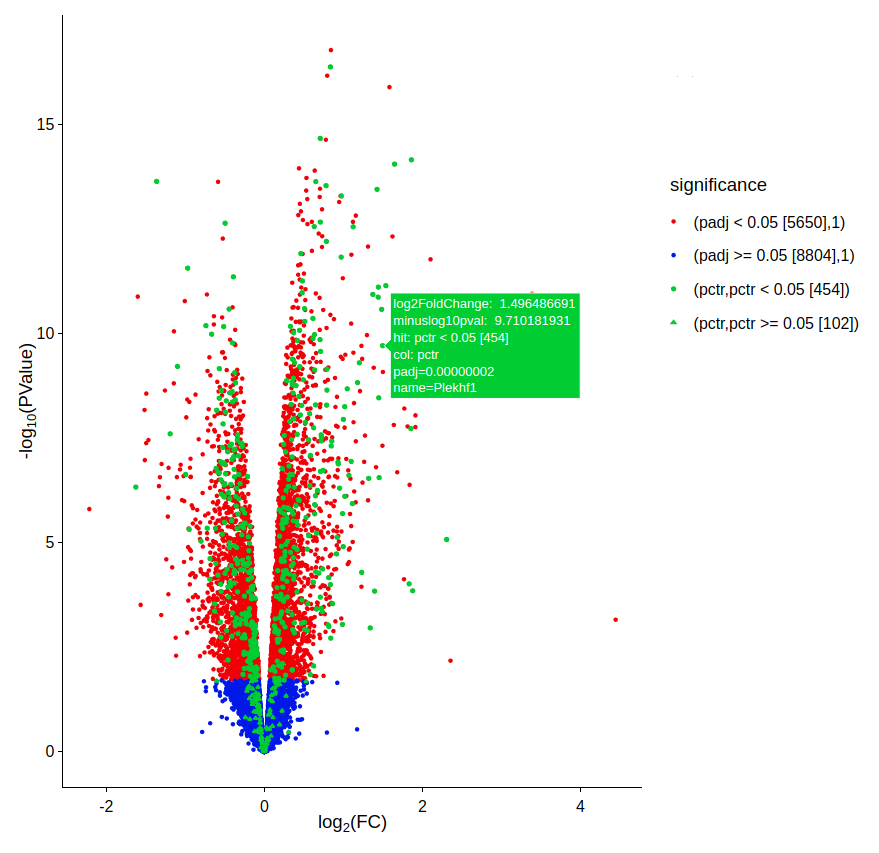
\includegraphics[width=\textwidth,height=\textheight,keepaspectratio]{img/ticorser/volcano_example.png}
\caption[ticorser volcano]{An example of interactive volcano plot made with \gls{tic} package. Each dot represents a gene, while blue and red colours highlights the significance of the genes. In green there are those genes coming from the positive control list. When passing the mouse over a dot it shows additional information about the selected gene.}
\label{fig:ticorservolcano}
\centering
\end{figure}

The MA-Plot puts in relation two quantities useful to understand the differences between the measurements in two conditions.
On the x-axis there is represented the $log_2(T/C)$ where \textit{T} is the treatement condition and \textit{C} its control.
It is not mandatory to have a DE results dataframe to plot an MA-plot, but it's pretty useful to have it in order to understand the distribution of the significant genes.
 

\begin{figure}[H]
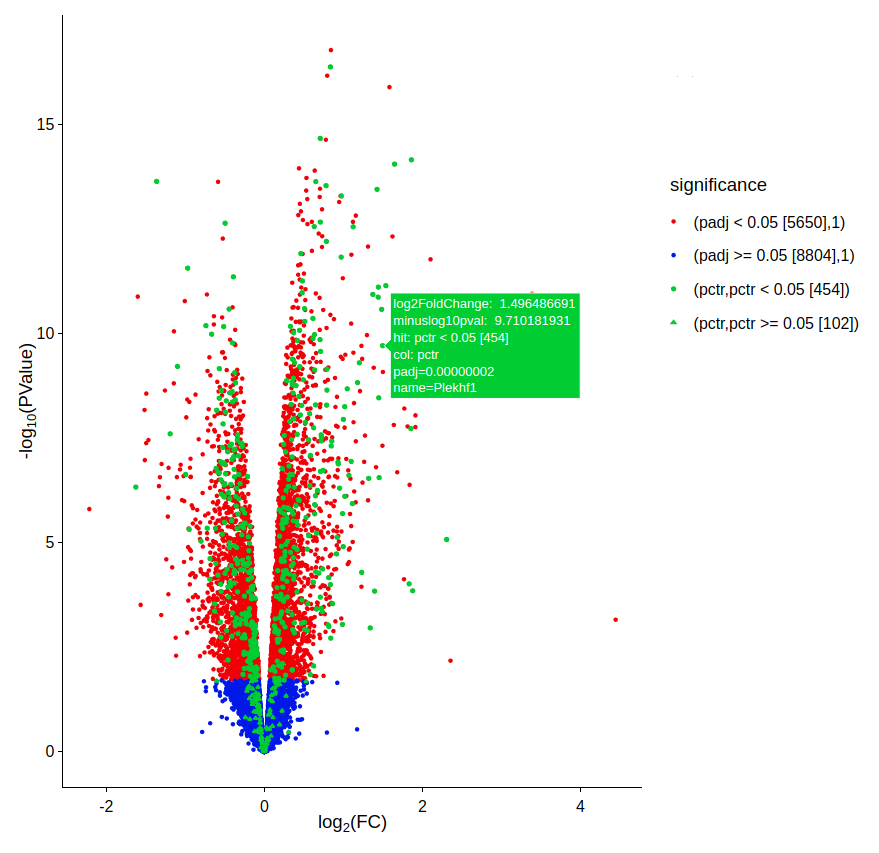
\includegraphics[width=\textwidth,height=\textheight,keepaspectratio]{img/ticorser/volcano_example.png}
\caption[ticorser MAplot]{An example of interactive MA-plot made with \gls{tic} package. Each dot represents a gene, while blue and red colours highlights the significance of the genes. When passing the mouse over a dot it shows additional information about the selected gene.}
\label{fig:ticorsermaplot}
\centering
\end{figure}


\subsubsection{Gene Profiles plot}
For highlighting the profile of a gene, we implemented the function \lstinline!plotGeneProfile!, where takes as input the count matrix, a gene name, and the design matrix.
In such a way the function is able to plot the profile of a gene showing its trend throught all time points, and between the different conditions.

\begin{figure}[H]
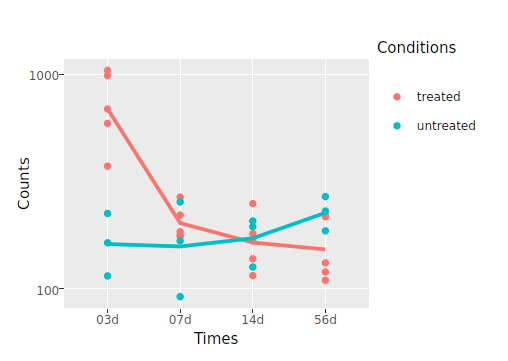
\includegraphics[width=\textwidth,height=\textheight,keepaspectratio]{img/ticorser/gene_trend.png}
\caption[ticorser gene profile]{An example of interactive gene profile made with \gls{tic} package. Each dot represents the counts value of the gene in a sample. Colours identifies the conditions of the samples. The lines represent the gene trend over all time points.}
\label{fig:ticorsergenetrend}
\centering
\end{figure}

\subsubsection{keggmap}
\gls{tic} offers the possibility to plot \textit{keggmaps}\cite{Kanehisa2016} taking into account the $log_2(FC)$ of the genes involved in the graphical representation, thought all the timepoints.
Indeed, using the \lstinline!plotKeggmap! function it enables to plot a \textit{keggmap}, using as input the counts and the design matrices, computing the $log_2(FC)$ at each time point, and showing it in the gene box inside the plot.

\begin{figure}[H]
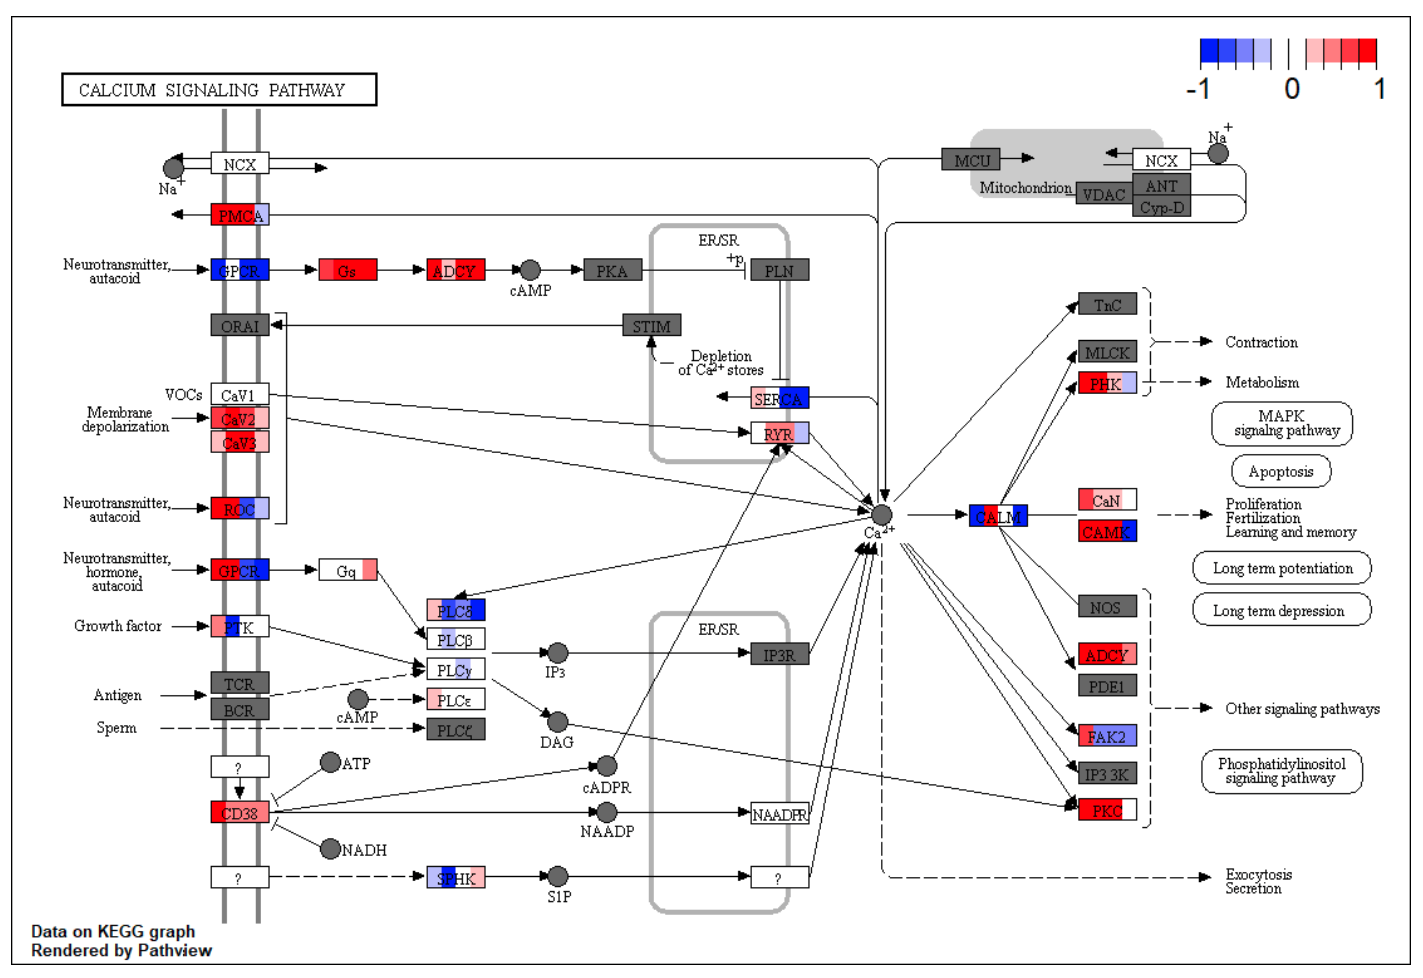
\includegraphics[width=\textwidth,height=\textheight,keepaspectratio]{img/ticorser/keggmap_example.png}
\caption[ticorser keggmap]{add description}
\label{fig:ticorserkeggmap}
\centering
\end{figure}









\section{Additional Features} \label{sec:ticorseraddfeat}
The package offers additional features for loading data (i.e. peaks) resulting from other sources, and for manipulating \textit{GenomicRanges} data structure.

The method \lstinline{readFilesAsGRangesList} takes as input a directory with BAM or BED data, to load in \textit{GenomicRangesList} format.
This data structure is useful to store genomic information, as peaks or mapped reads, produced by other software like \textit{MACS2} or \textit{STAR} and, in case of peaks, it is necessary during the \gls{descan} filtering step.
Additionally to \lstinline{fileType} (BAM, BED, BED.zip) parameter specification it requires the genome code to use during the file processing.
Moreover, when the input files represent peaks the \lstinline{arePeaks} flag needs to be set to \lstinline{TRUE}.
In such a way the \gls{descan} package can work also with data coming from other sources, preferred by the user.

Furthermore, \gls{descan} provides several functionalities for GenomicRanges data structure
handling. One over the others (\lstinline{fromSamplesToChrsGRangesList}) gives the possibility to split a GenomicRangesList by the chromosomes. 
This procedure could be useful for parallelizing the computations on the chromosomes, assigning a single chromosome to a single computing unit.
Taken as input a GenomicRangesList organized by samples, this method returns a list of chromosomes, where each element has a GenomicRangesList of samples, containing only the regions associated to the single chromosome.

[Create figure to better explain the transformation]

Other useful utilities are \lstinline{keepRelevantChrs}, that takes a GenomicRangesList and a list of chromosomes and return only the interested chromosomes.
\lstinline{saveGRangesAsTsv} that saves a tab separated value file starting from a GenomicRanges.
\lstinline{saveGRangesAsBed} that save a standard BED file format starting from a GenomicRanges data structure.
\lstinline{setGRangesGenomeInfo} which, starting from a genome code, sets a specific \textit{genomeInfo} to a \textit{GenomicRanges} object.
\section{Case Study} \label{sec:ticorseresults}
\textbf{Few words on ATAC-Seq data}

We illustrate the performances of \gls{descan} using a dataset \cite{Su2017} that describes in vivo adult mouse dentate granule neurons before and after synchronous neuronal activation using Atac-Seq and RNA-Seq technologies (see sections \ref{sec:atacseq} and \ref{sec:rnaseq} for a description of these sequencing techniques).

This dataset is organized in 62 samples of Atac-Seq and RNA-Seq, extracted at different time points, with four replicates at each time point.
We chose to compare the differences btween the first two stages, time 0 (E0) and 1 hour after neuronal induction (E1), in order to show a possible Atac-Sec workflow for Differential Enrichment, and how to integrate this data type with RNA-Seq. A general illustration of our dataset is represented in figure \ref{fig:atacdataset}.

\begin{figure}[H]
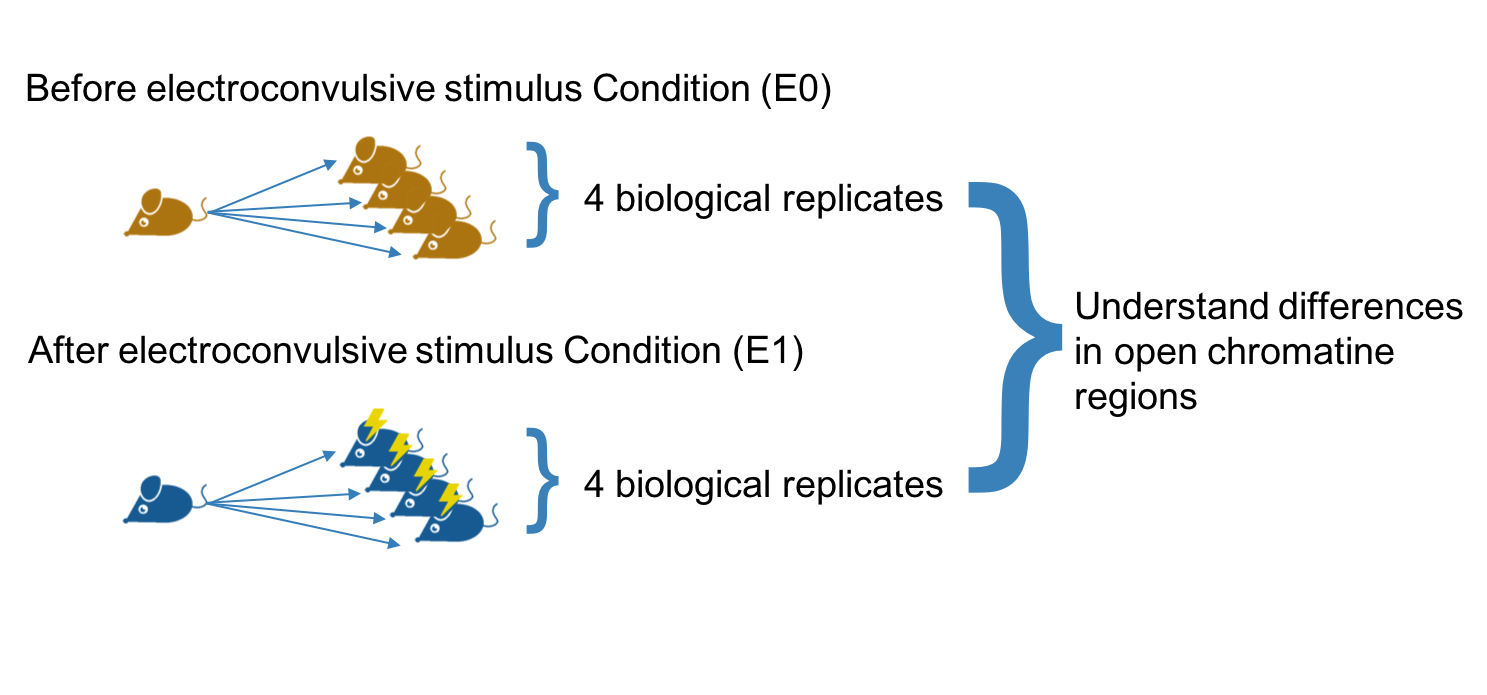
\includegraphics[width=\textwidth,height=\textheight,keepaspectratio]{img/descan2/dataset.png}
\caption[DEScan2 dataset illustration]{An illustration of our extraction of the \cite{Su2017} dataset.}
\label{fig:atacdataset}
\centering
\end{figure}

We downloaded the data from \gls{geo} database \cite{Edgar2002, Barrett2013} with accession number GSE82015\footnote{\url{https://www.ncbi.nlm.nih.gov/geo/query/acc.cgi?acc=GSE82015}} and mapped raw data using \textit{STAR} \cite{Dobin2013} with default parameter on \gls{mm10}.

In order to detect the open chromatin regions we run our peak caller, cutting the genome in bins of 50bp and using running windows of minimum 50bp and maximum 1000bp. In such a way we are able to detect not just broad peak, but also smaller peaks.

To be confident with our results we compared the \gls{descan} detected peaks with the same validated regions (Arc and Gabrr1) in the original work \cite{Su2017}.
The lower part of figure \ref{fig:peaksdescan} shows the detected and validated regions (in blue and red) resulting differentially enriched between the E0 (in pink) and E1 (in green) conditions, while the upper part shows \gls{descan} peaks (in blue), highlighting a capability to catch not only the same regions of the published ones, but also (gold circles) to be more careful in the smaller peaks detection.

\begin{figure}[H]
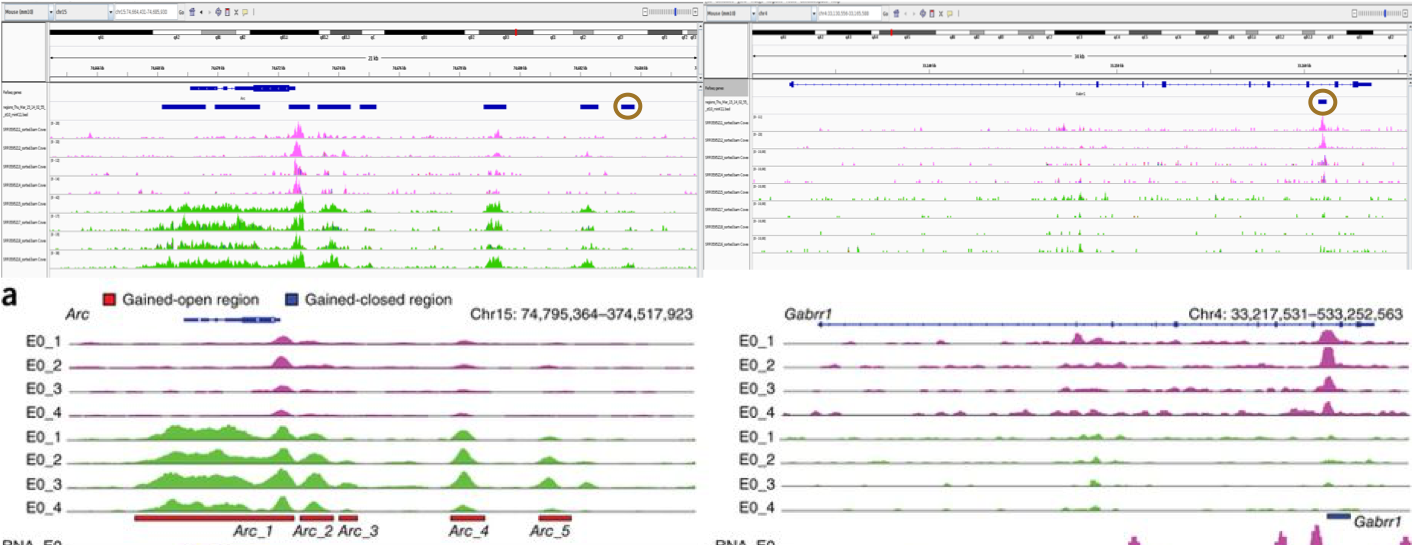
\includegraphics[width=\textwidth,height=\textheight,keepaspectratio]{img/descan2/peaks.png}
\caption[\gls{descan} peaks detection]{A comparison of \gls{descan} detected peaks with validated peaks in article \cite{Su2017}.}
\label{fig:peaksdescan}
\centering
\end{figure}

Moreover, we run \textit{MACS2} on the same samples, and (as shown in figure \ref{fig:des2m2peaks}) \gls{descan} seems able to catch much more peaks than \textit{MACS2} for each sample.

\begin{figure}[H]
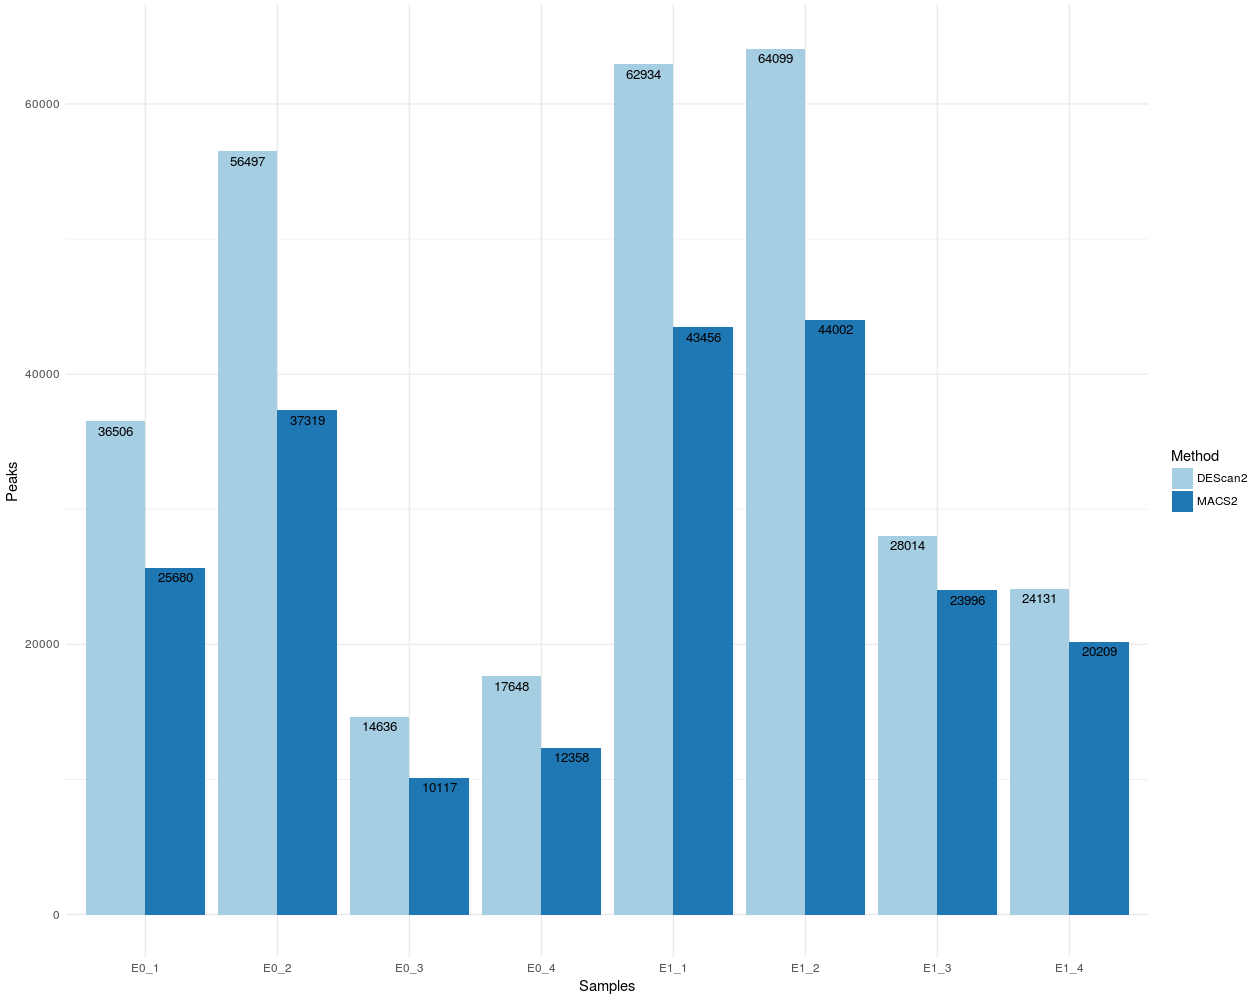
\includegraphics[width=\textwidth,height=\textheight,keepaspectratio]{img/descan2/d2m2_peaks_number.png}
\caption[The \gls{descan} and \textit{MACS2} peaks detection]{A comparison of \gls{descan} and \textit{MACS2} detected peaks for each sample in the dataset.}
\label{fig:des2m2peaks}
\centering
\end{figure}

While it is very important to detect good peaks with a peak caller, it seems to be more relevant to detect reliable regions. Indeed, during the filtering step, the number of peaks depends not only by the peak score, but also by the number of replicates designed in the experiment.
The figure \ref{fig:filteringdescan} puts in relation these two relevant information. 
On the x-axis is represented the number of replicates, while on the y-axis is traced the number of peaks, and each curve represents a different threshold on the peaks score, showing that higher are the thresholds on the scores and the number of replicates, lower is the number of the detected peaks.
Highlighting a proportional inversion between the number of the peaks and the combination of the number of samples and the detected regions score.


\begin{figure}[H]
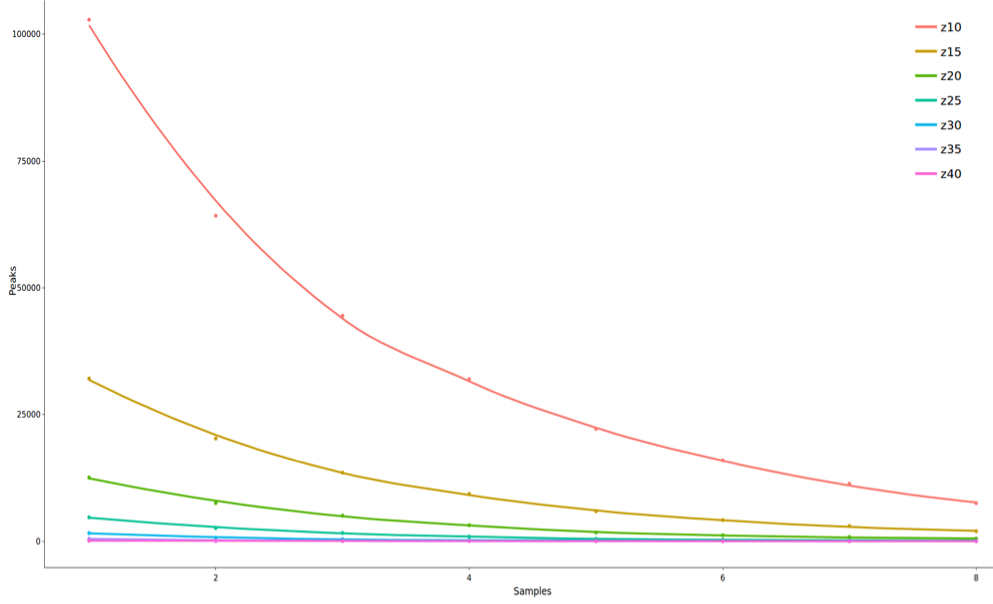
\includegraphics[width=\textwidth, height=\textheight, keepaspectratio]{img/descan2/filtering.png}
\caption[\gls{descan} filtering step]{Filtering the detected regions with different thresholds on peak scores.}
\label{fig:filteringdescan}
\centering
\end{figure}


\begin{figure}[H]
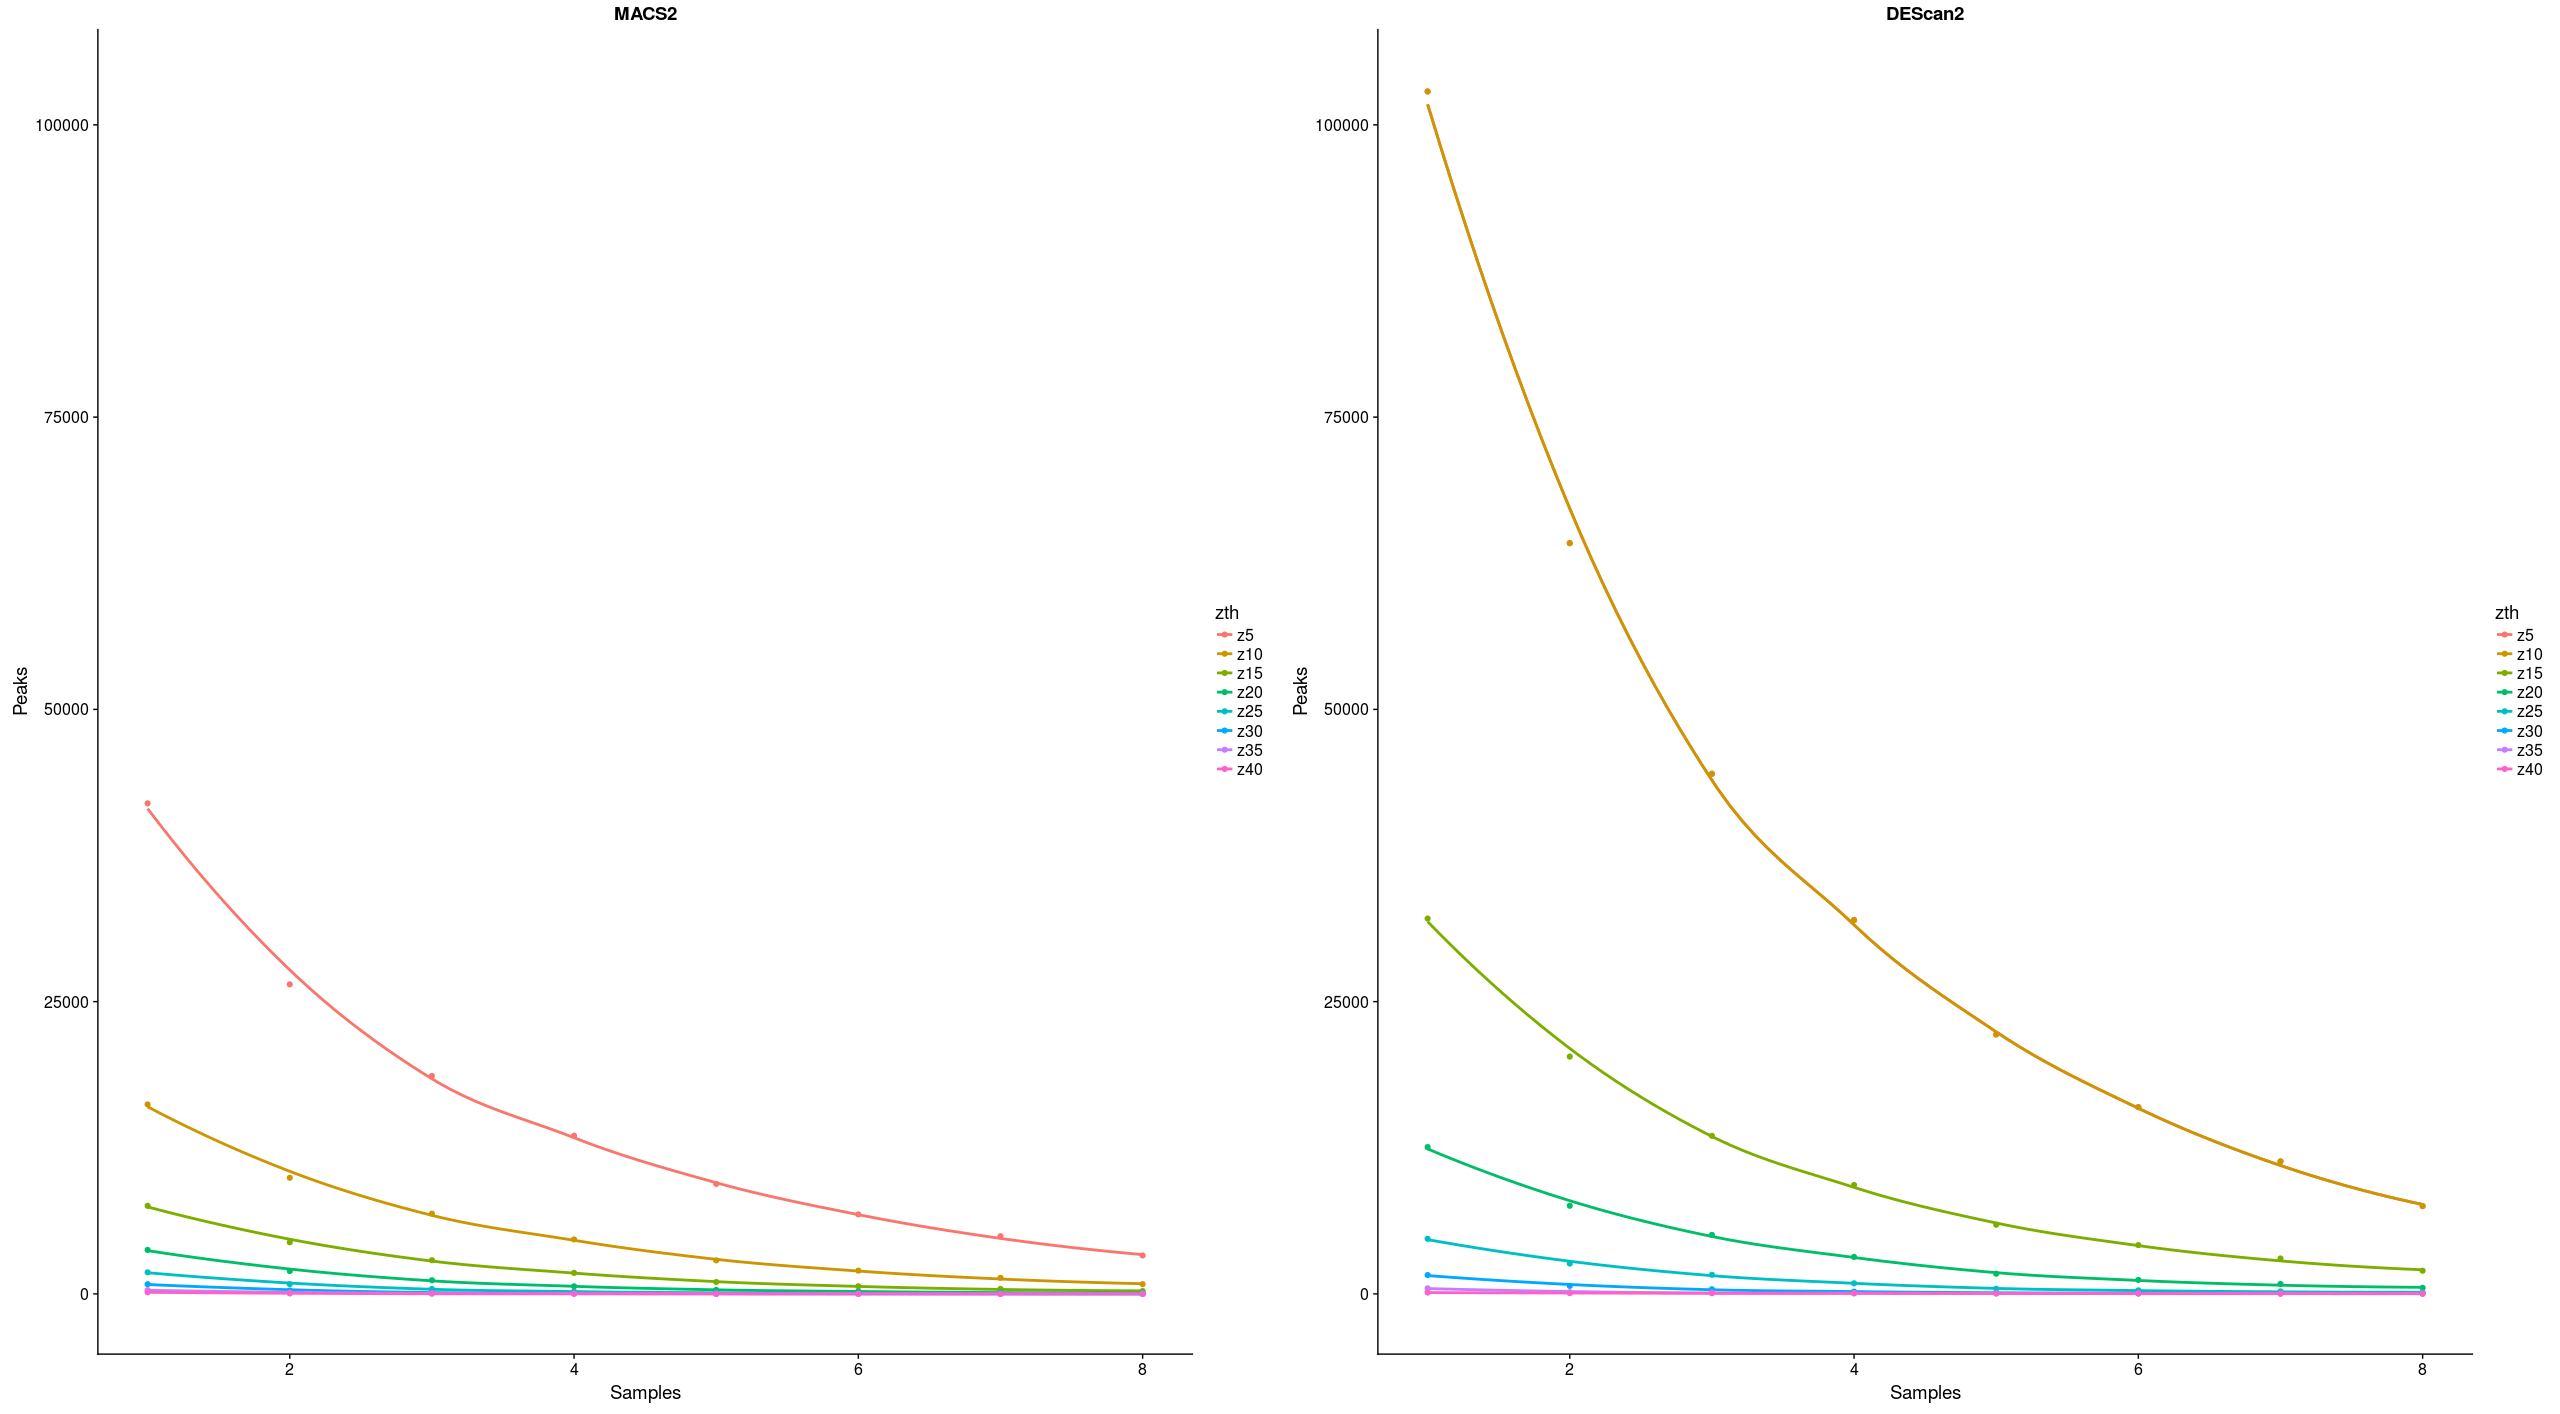
\includegraphics[width=\textwidth, height=\textheight, keepaspectratio]{img/descan2/filtering_m2_d2.png}
\caption[\gls{descan} and \textit{MACS2} filtering comparison]{Filtering the detected regions with different thresholds on peak scores between \textit{MACS2} and \gls{descan}.}
\label{fig:filteringdescanmacs2}
\centering
\end{figure}

The filtered-in regions can be processed by \gls{descan} in order to obtain a count matrix with samples on the columns and peaks on the rows.
This type of data structure is very versatile, because it enables to perform several operations, like the \glspl{der} and, if possible, the integration with other kind of omics, as RNA-Seq.

In order to preserve the information associated to the peaks, \gls{descan} produces as output a \textit{SummarizedExperiment} (figure \ref{fig:countsdescan}) data structure, which enables to retrieve the count matrix with \lstinline{assays} method, and to access the peaks information in \textit{GenomicRanges} format with the \lstinline{rowRanges} method. %{

\begin{figure}[H]
\centering
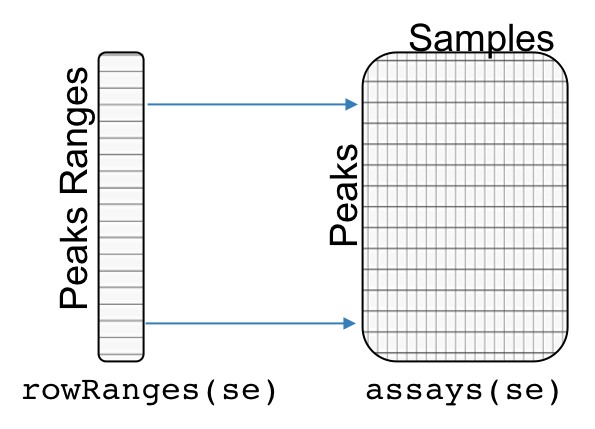
\includegraphics[keepaspectratio]{img/descan2/counts.png}
\caption[\gls{descan} counts illustration]{An illustration of the \textit{SummarizedExperiment} data structure produced by \gls{descan}.}
\label{fig:countsdescan}
\centering
\end{figure}

Before to proceed to detect \glspl{der}, it is a good standard to normalize the data, also because without any kind of normalization we are not able to detect any \gls{der}.
The nature of the data, in count format, makes it possible to apply several well known RNA-Seq normalizations techniques, as \textit{TMM}, \textit{upper-quartile}, \textit{full-quantile}, \textit{RUV-Seq}, etc \cite{Risso2014, Robinson2010, Dillies2013}.

While the \textit{TMM} and \textit{upper-quartile} normalizations modify the data in a way that makes it impossible to detect \glspl{der}, other kind of normalizations and combinantions of them give good results.

The figure \ref{fig:normalizationsdescan} sintetizes this concept very well, highlighting a relation between the number of \glspl{der} and the minumum number of samples used for filtering the data during the \gls{descan} filtering step.

The plot shows that \textit{upper-quantile}, even if combined with \textit{RUV-Seq} normalization, is not able to linearly detect a good amount of \glspl{der}, while \textit{full-quantile}, when combined with \textit{RUV-Seq} seems to affect the data in a way that overdetect the number of \glspl{der}. 
When looking at the \textit{full-quantile} and \textit{RUV-Seq} by themself seem to perform better than the other normalizations. The first one has a downhill almost linear, while the second one has a very fast downhill with a regrowth when the number of samples is higher.

Even if these normalization methods show good performances with this type of epignomic data, our investigations suggest that more testing is required, but maybe an ad-hoc normalization method for these data has to be developed.

\begin{figure}[H]
\centering
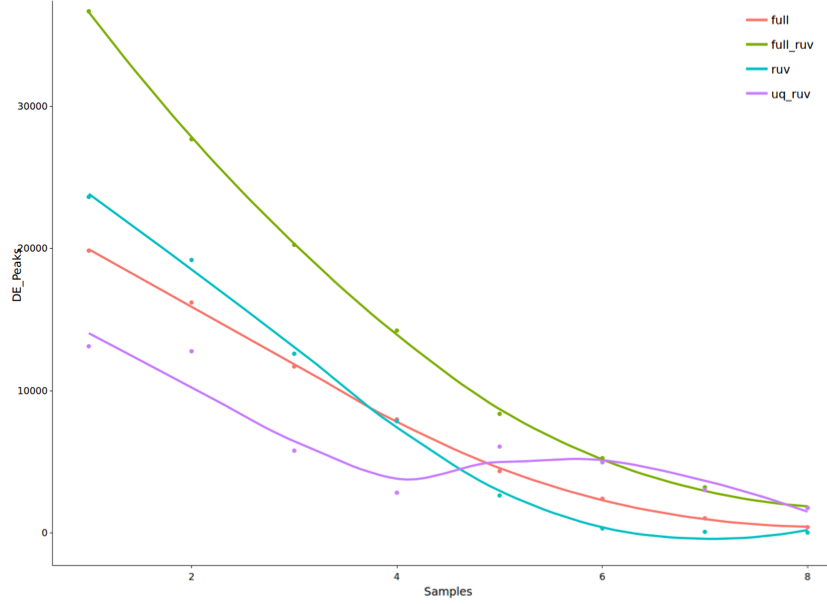
\includegraphics[width=\textwidth, height=\textheight, keepaspectratio]{img/descan2/normalizations.png}
\caption[Normalizations applied to detected regions]{The figure shows the effects of different normalizations on the epigenomic differentially enriched regions.}
\label{fig:normalizationsdescan}
\centering
\end{figure}

To estimate the \glspl{der}, any of the RNA-Seq methods can be applied, such as \textit{DESeq2}, \textit{edgeR}, \textit{NOISeq}, etc \cite{Robinson2009, McCarthy2012, Tarazona2012}.

In this case, we decided to use \textit{edgeR} package, because of its wide range of  available statistical approaches and the possibility to better tune the design of the experiment. 
Indeed, because we used the RUV-Seq normalized counts with \lstinline{k} parameter set to 4, we modeled the experimental design with the \lstinline{model.matrix} function, adding to our model not only the experimental conditions, but also the RUV-Seq estimated weights.
Then we used the resulted design to estimate the dispersion and fit a Quasi-Likelihood test, as defined in edgeR.

The figure \ref{fig:depeaksdescan} shows a volcano plot of \glspl{der} between E0 and E1 conditions.
Red dots highlights the regions with a False Discovery Rate (FDR) lower than 0.05, while blue dots highlight not significant regions.
 
\begin{figure}[h]
\centering
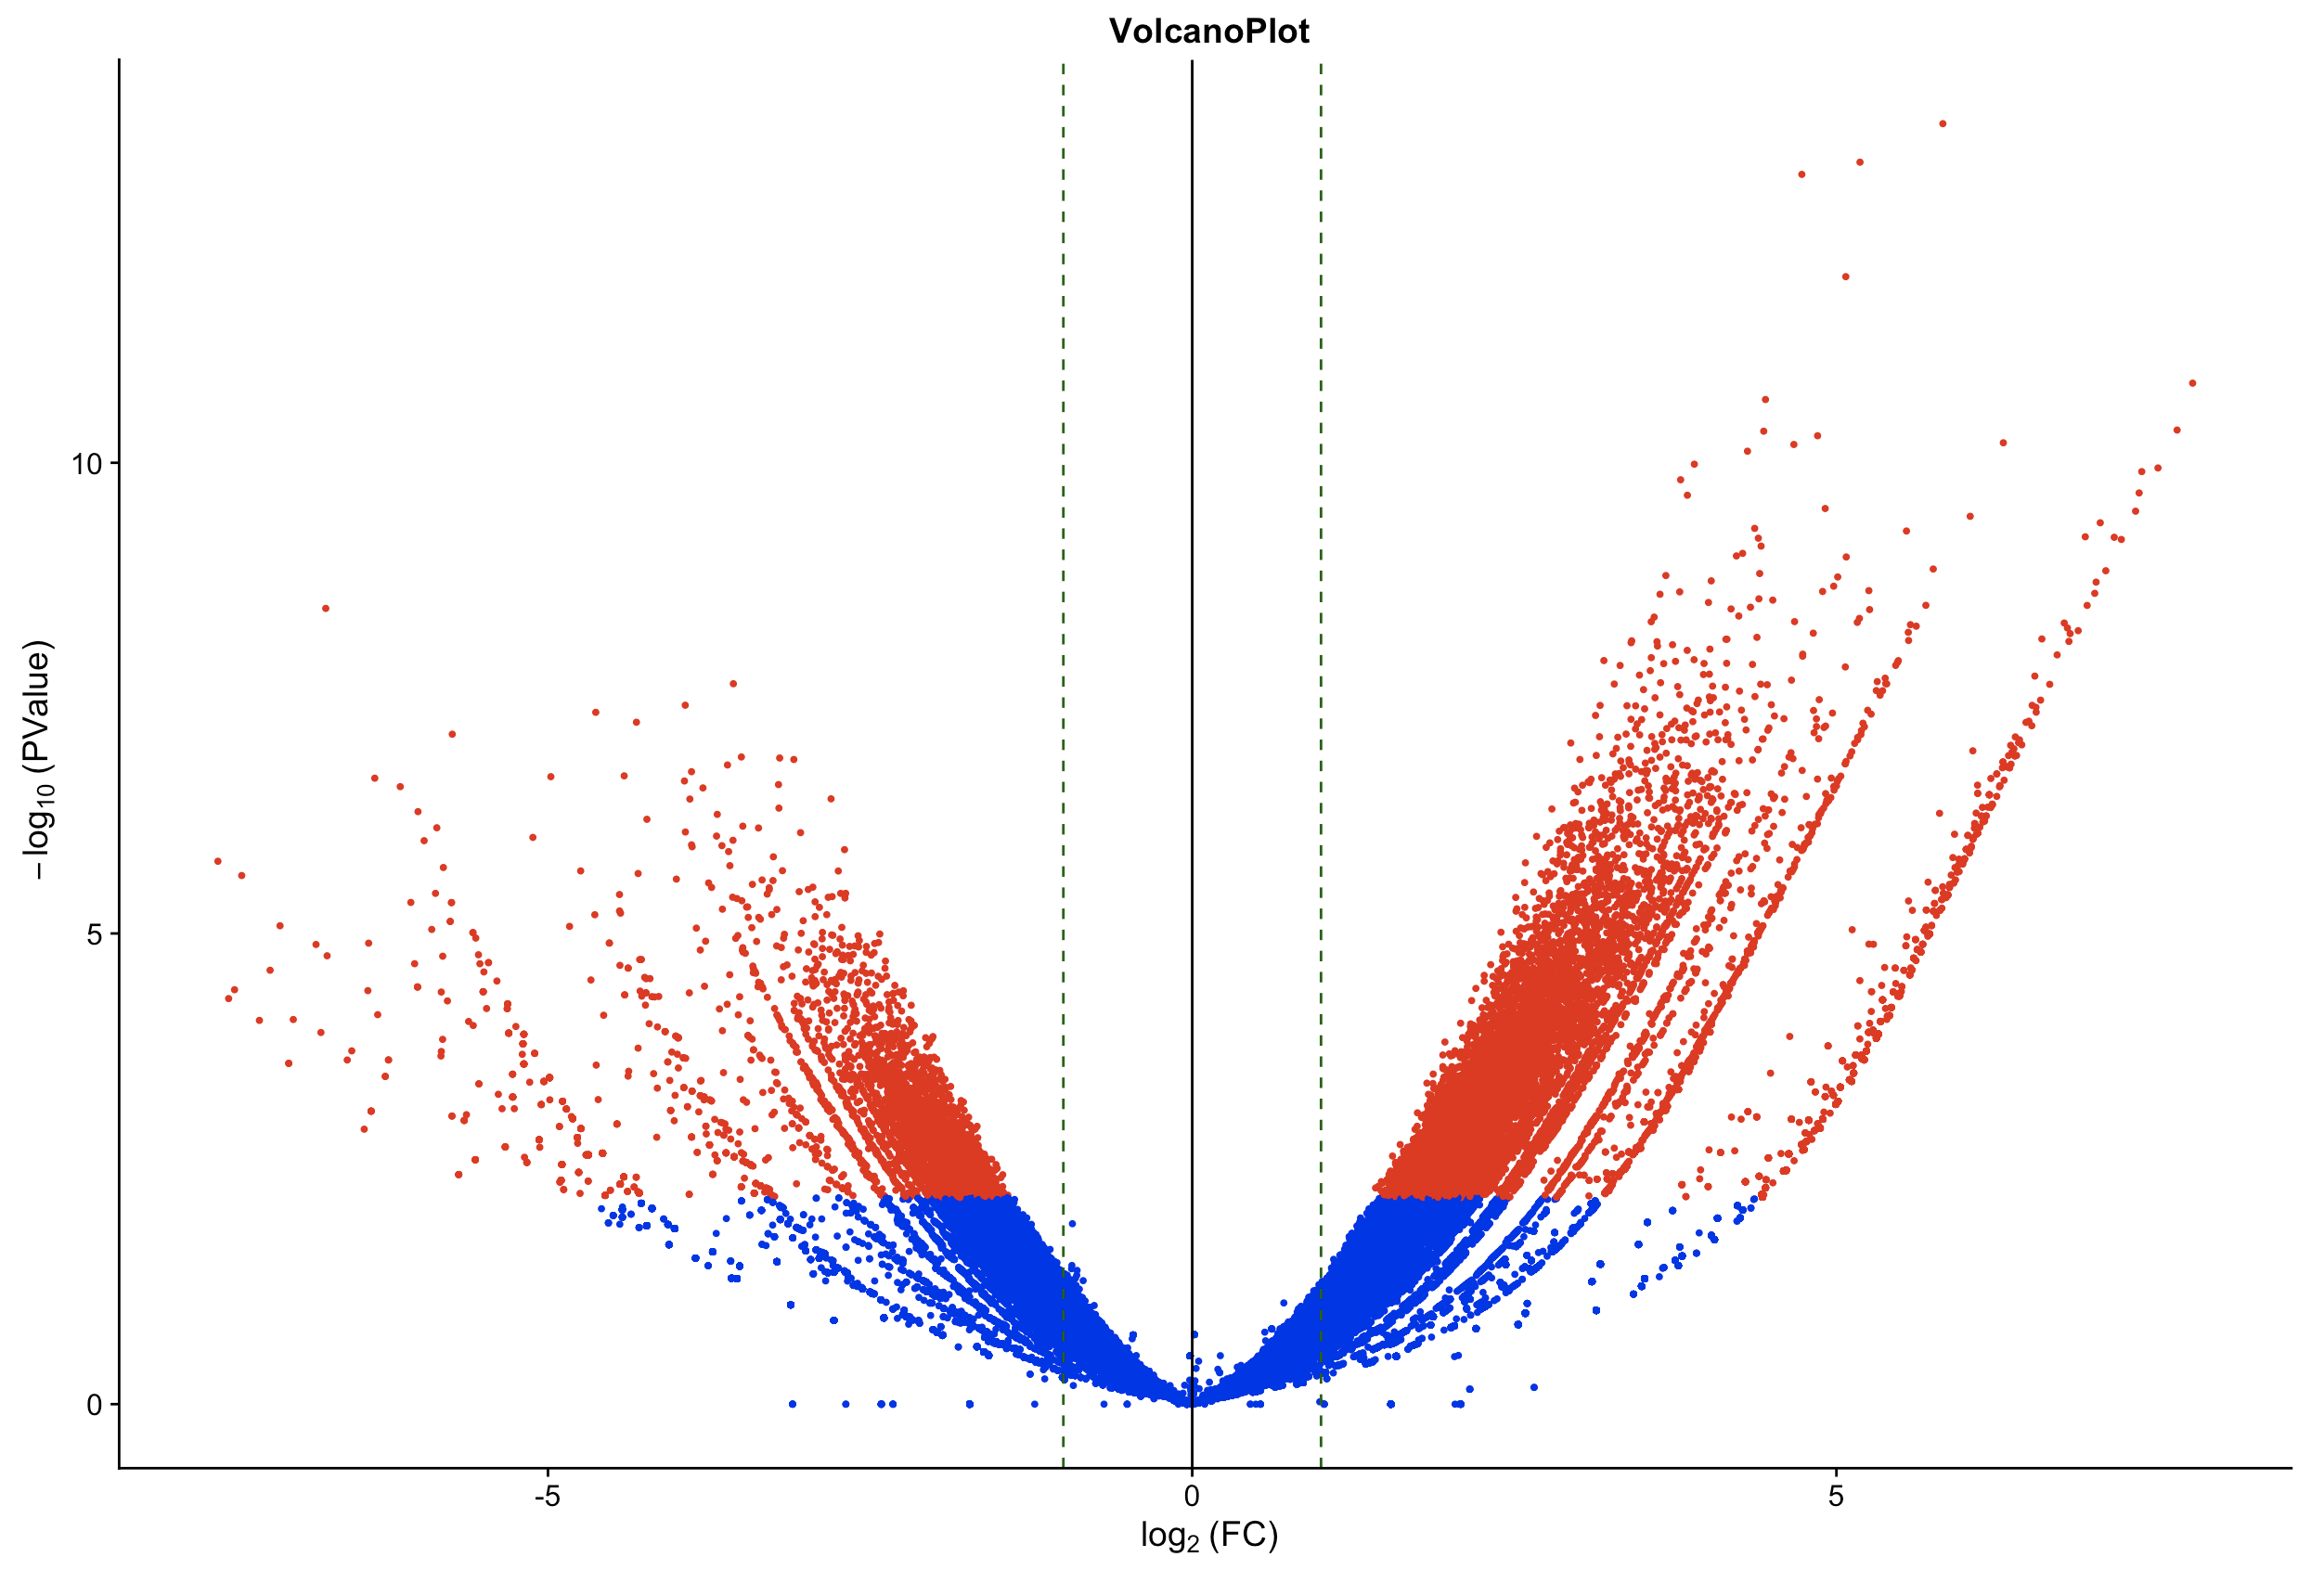
\includegraphics[width=\textwidth, height=\textheight, keepaspectratio]{img/descan2/DE_peaks.png}
\caption[Differential Enrichment Regions Volcano]{A volcano plot of Differential Enriched Regions. Blue dots represent the not significant \glspl{der}, while the red ones represent the significant \glspl{der}.}
\label{fig:depeaksdescan}
\centering
\end{figure}

Next task is to integrate the obtained results with other omic data types, as RNA-Seq. 
Because of the low number of the samples, the easiest way to integrate the data is to annotate the \glspl{der} with differentially expressed genes resulting from the analysis of RNA-Seq.

For the Differential expression of the RNA-Seq data we firstly quantified the signal with \lstinline{featureCounts} methods available in the \textit{Rsubread} \cite{Liao2013} Bioconductor package.
Then we filtered lowly expressed genes with the \textit{proportion} test  as implemented in \textit{NOISeq} package, and applied the \lstinline{noiseq} method for differential expression.%{

\begin{figure}[h]
\centering
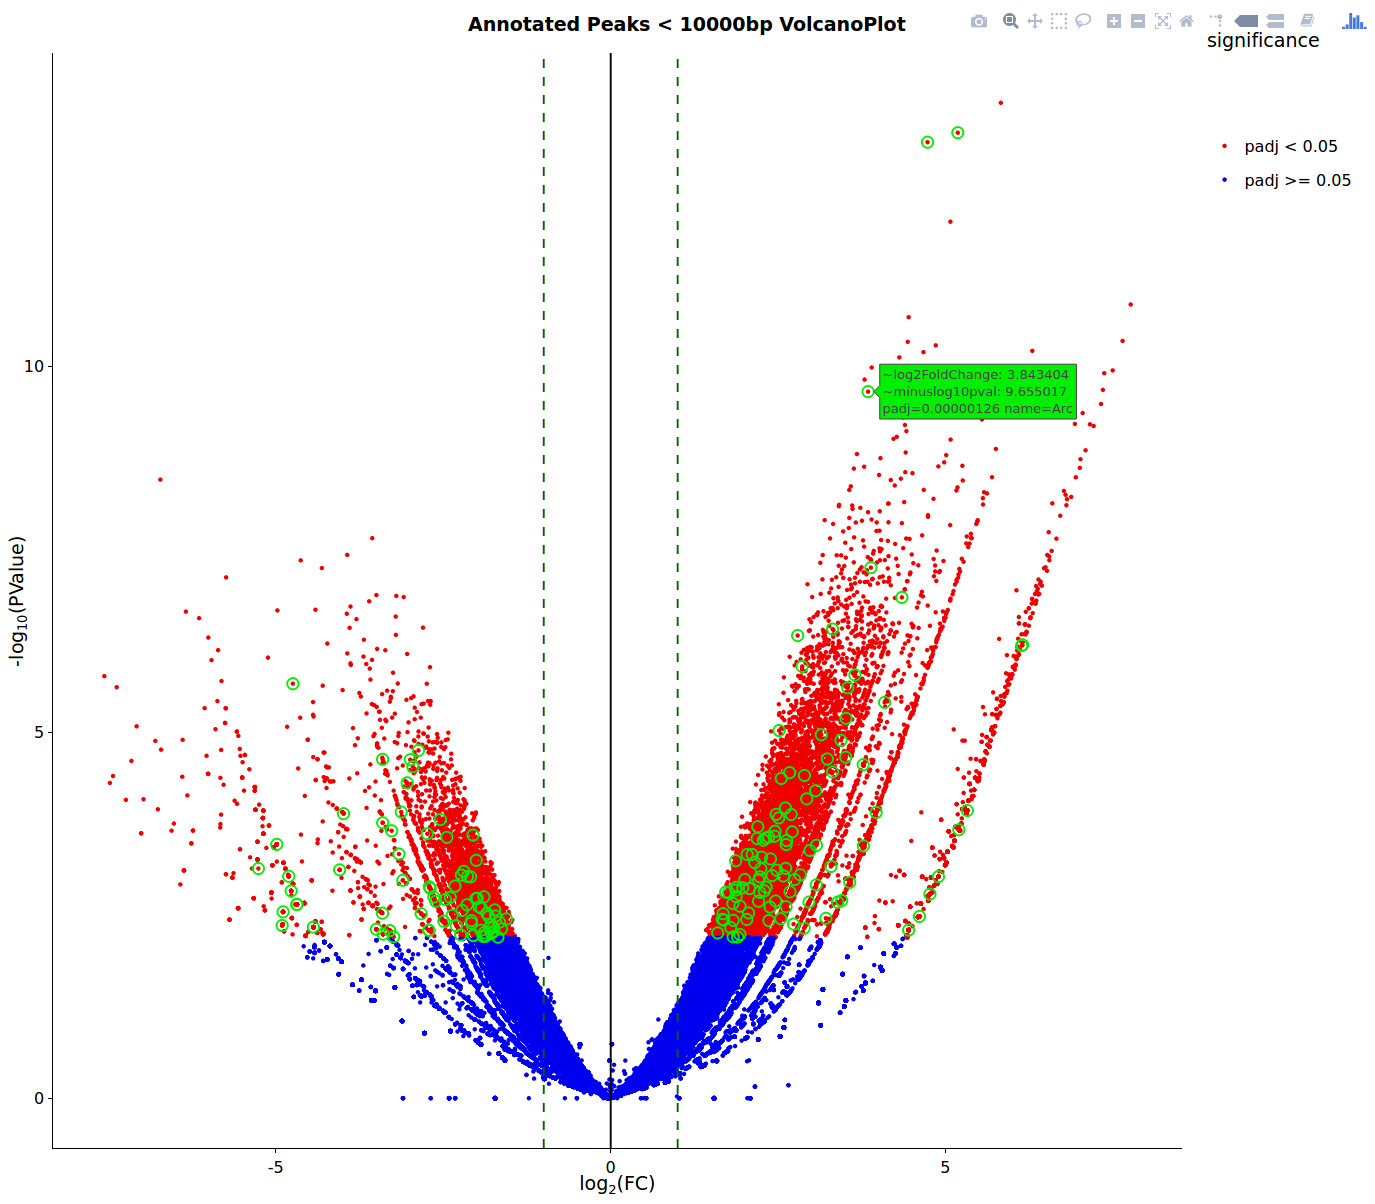
\includegraphics[width=\textwidth, height=\textheight, keepaspectratio]{img/descan2/Annotated_depeaks_degenes.png}
\caption[Annotated Differential Enrichment Regions Volcano]{A volcano plot of \glspl{der}. Blue dots represent the not significant \glspl{der}, while the red ones represent the significant \glspl{der}. Green circles highlights the peaks with a \gls{deg} annotated.}
\label{fig:depeakdegenessdescan}
\centering
\end{figure}

We selected the significant \glspl{deg} with a probability higher than 0.95, and used these genes to annotate the peaks with \lstinline{annotatePeakInBatch} method of ChIPpeakAnno.
Figure 	\ref{fig:depeakdegenessdescan} illustrates with green circles the peaks with an annotated gene with distance lower than 10000bp from the gene TSS.
Realizing the plot with the \textit{plotly} library it's possible to enhance the names of the genes with a tip window.










\section{Discussions} \label{sec:ticorseconclusions}
Multiple omics data information extraction became always more complex with the evolution of sequencing techniques and with the consequent development of methodologies for their analysis and integration.
With this thesis work, we focused on the development of novel strategies for several problems related to multiple omics sequencing data information extraction.

Firstly, we approached the most studied genomic problem, transcriptomic, by focusing on time-course \textit{RNA-seq} data.
We presented \textit{ticorser}, an R command line package for time-course \textit{RNA-seq} data.
With this instrument we propose a complete pipeline for the time-course data analysis, presenting also ad-hoc designed approaches for this type of data visualization at different levels.
Additionally, allowing a first integration level with functional annotation and also for their visualization.

Afterwards, we focused on \textit{ATAC-seq} technology, an emerging technique for open chromatin region detection, which still needs appropriate solutions for its analysis.
To address the lack of methodologies with this data we presented \textit{DEScan2}, an R/Bioconductor package allowing detection of open chromatin regions, and proposed a possible workflow for the detection of \glspl{der} and their integration with \textit{RNA-seq} data.

Due to the difficulty of keeping track even a single omic analysis, we presented \textit{easyReporting}, a possible approach to the Reproducible Research inside R.
A tool which helps not only software developers to include \gls{rr} layers inside their tools, but also non-expert R analysts to easily produce reports for their analysis.

Finally, to speed up and help also non-expert users to analyze multiple omics data, we presented \gls{igro}, a web graphical user interface for the analysis of omics data.
Combining the flexibility of a point-and-click approach with the power of R/Bioconductor statistical approaches for the omics data analysis.
Moreover, thanks to the Reproducible Research layer it allows to keep track of all the steps performed during the analysis, and with aid of dedicated interface to live edit the enriched report.

%%%%%%%%%%%%%%%%%%%%%%%%%%%%%%%%%%%%%%%%%%%%%%%%%%%%%%%%%%%%%%%%

\chapter{Differential Enriched Scan 2: DEScan2} \label{sec:descan2cap}

\textbf{\textsl{few words on integration of epigenomic with transcriptomic}}

To investigate and answer epigenetic biological questions we decided to create a useful instrument for analysing epigenomic data (such as \textit{ChIP-Seq}, \textit{Atac-Seq}, \textit{Sono-Seq}).
Very often the biological questions to be answered, as for the RNA-Seq, need the comparison of two or more different biological conditions.
Starting from a set of already published \cite{Koberstein2018} scripts, we designed \textit{Differential Enriched Scan 2} (\textit{DEScan2}), a software for helping the analysis of epigenomic data.
\section{Introduction} \label{sec:descan2intro}
In order to deeply understand and reconstruct cellular mechanisms influenced by drug treatments, pathologies or diseases, it is fundamental to look at multiple omics data types at the same time.

Previous chapters deeply described tools for multiple omics data analysis, integration and visualization using command line tools.
Even if the command line approach is pretty common inside the bioinformatics community, it is not for every scientist who is not so confident with programming languages or terminal.
When working with multiple omics data, there is an overabundance of available tools for each sequencing that can bewilder a beginner, up to the point to renounce approaching the analysis problem.

%Moreover, thanks to our previous experiences \cite{russo2015advantages} in developing \gls{gui}, we noticed a growing interest by the scientific community in using interactive software.
%This interest seems to be leaded by multiple motivations, such as the need to analyze data very fast or the lack of time in learning programming languages and terminal-line based tools.

Furthermore, even if the bioinformatics community has massively moved on the development of novel statistical and computational methods for multi-omics data integration, part of the scientific community is still anchored to the single-omics analysis side.
Even if still really helpful, it is still very common to read published papers based on single-omics data analysis without taking into account possible integrated solution with other omics data types.

Of course, it is not so simple to afford for multiple omics data experiments, but, nowadays, the internet swarms of public datasets.
In particular when looking at public biological data banks, such as \gls{geo}\footnote{\url{https://www.ncbi.nlm.nih.gov/geo/}} \cite{Services2007} or \gls{tcga}\footnote{\url{https://cancergenome.nih.gov/}} \cite{tcga2013a}, where it is possible to retrieve as many data as needed.

On the other side, if there are not so many papers publishing integrated analysis, it is also difficult for analysts to retrieve the right methodologies for the multi-omics data analysis and their visualization. 

\begin{figure}[H]
\centering
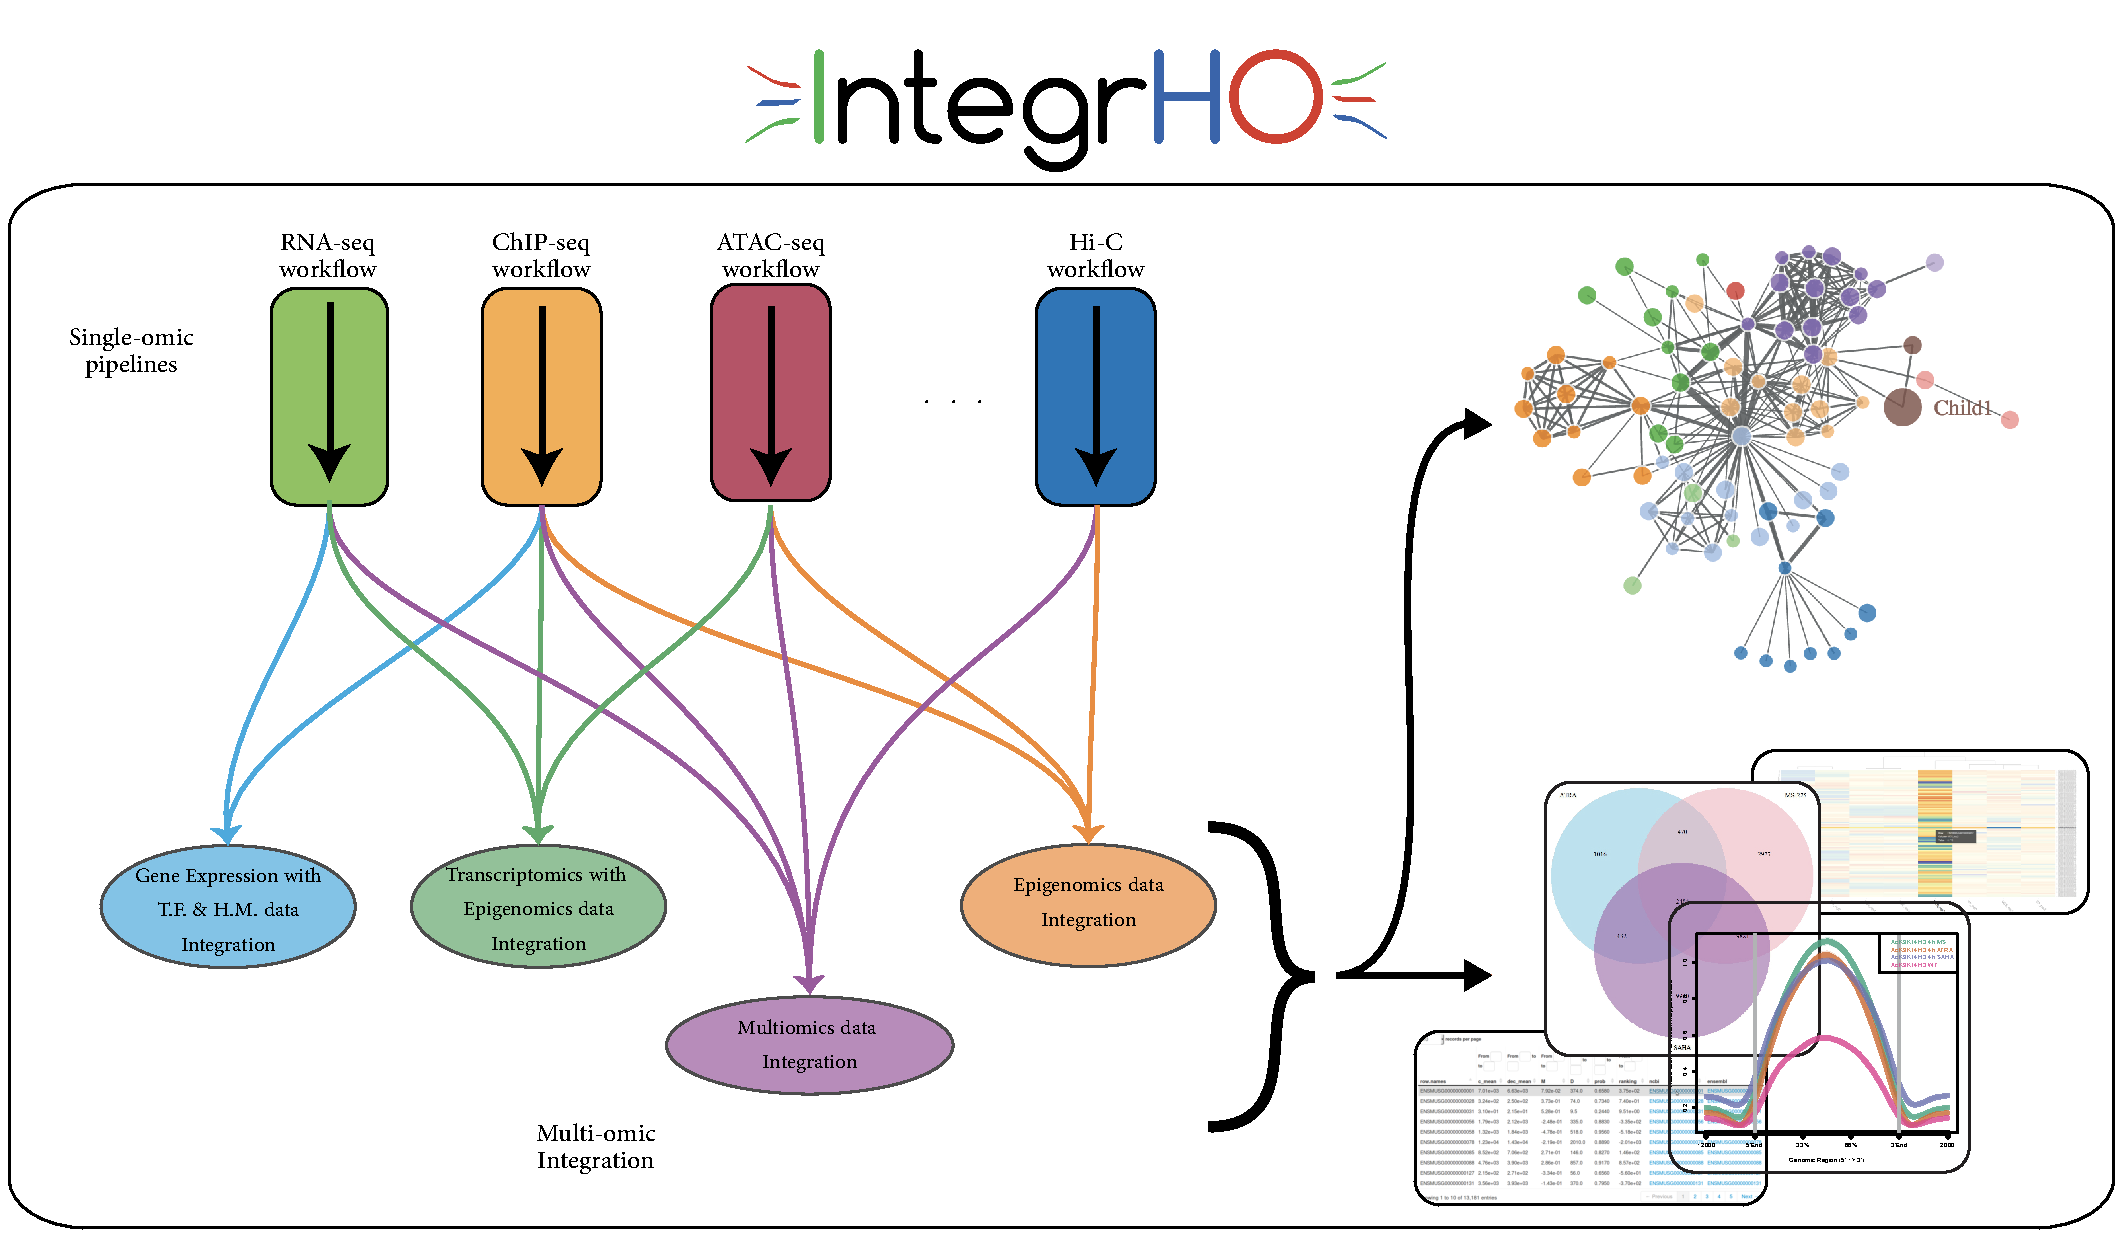
\includegraphics[width=\textwidth, keepaspectratio]{img/integrho/integrho_scheme.pdf}
\caption[\gls{igro} representation]{A schematical representation of \gls{igro} underlying idea.
Single-omics analysis methods are proposed in order to facilitate their multiple integration.
This integration can lead to produce graphical results, in case of low dimension datasets, or to more sophisticated integration model such as regulation networks, in case of high-dimension datasets.}
\label{fig:integrhoidea}
\end{figure}

Based on these considerations and in order to promote the multi-omics data integration, we decided to provide the scientific community of a novel easy-to-use instrument which not only gives the possibility to analyze single-omics data types but also guides the user through multiple ways of integrating multi-omics data types (figure \ref{fig:integrhoidea} gives an underlying idea of \gls{igro}).





%Several interface-based tools \cite{Poplawski2016} have been proposed during last years but too often they are oriented to analyze singular-omics or when designed for multi-omics, they are pipeline oriented. 

%In this chapter we introduce \gls{igro}, our web-based platform for multi-omics data analysis and integration,  in a \gls{rr} spirit.



\section{Methods} \label{sec:descan2methods}
Here we present \textit{easyReporting}, an \textit{R6} \footnote{\url{https://adv-r.hadley.nz/r6.html}}\footnote{\url{https://cran.r-project.org/web/packages/R6/index.html}} class\footnote{\url{https://en.wikipedia.org/wiki/Class_(computer_programming)}} developers to integrate a reproducible research layer inside their software products, as well as lazy analysts to speed up their report production without learning the \textit{rmarkdown} language.

In such a way, thanks to minimal additional efforts of developers, the end user has available an \textit{rmarkdown} file within all the source code generated during the analysis, divided into \glspl{cc} ready for the compilation.

Once manually edited with comments and descriptions the file can be compiled to produce an enriched document within input data, source code and output results.

A so final document can be attached to the publication of the analysis as supplementary material, helping the interested community to entirely reproduce the computational part of work (figure \ref{fig:rrscheme}). 

The package is accessible at the following link:\\ \href{https://github.com/drighelli/easyreporting}{https://github.com/drighelli/easyreporting} 

\subsubsection{General Description and Initialization}

The class can to be imagined as a schematic representation of the \textit{rmarkdown} file (\textit{report}), indeed 
its attributes represent the \textit{report} characteristics, which are typically inserted in the header of the file.
But our class methods are not only for the attributes manipulations but also for insertion of \glspl{cc}, comments and section titles inside the \textit{report}.

As any typical class, before of using it, \textit{easyReporting} requires to be initialized with the \lstinline!new! command, passing as mandatory arguments the \textit{path} and the name of the file as \lstinline!filenamepath! and a title as \lstinline!mainTitle!.
Additionally, an \lstinline!author! and the \lstinline!documentType! can be specified.

When initializing, the class automatically creates the \textit{report} with the entire specified folder tree, setting up the header of it and declaring the general options for the \textit{rmarkdown} file.
If \textit{rmarkdown} personal options (see figure \ref{fig:knitropts} for a list of available options) are required, before creating an instance of the class, it is possible to use the \lstinline!makeOptionsList! function, and then assigning the output to the \lstinline!optionsList! argument of the class \lstinline!constructor!.

\begin{figure}[H]
\centering
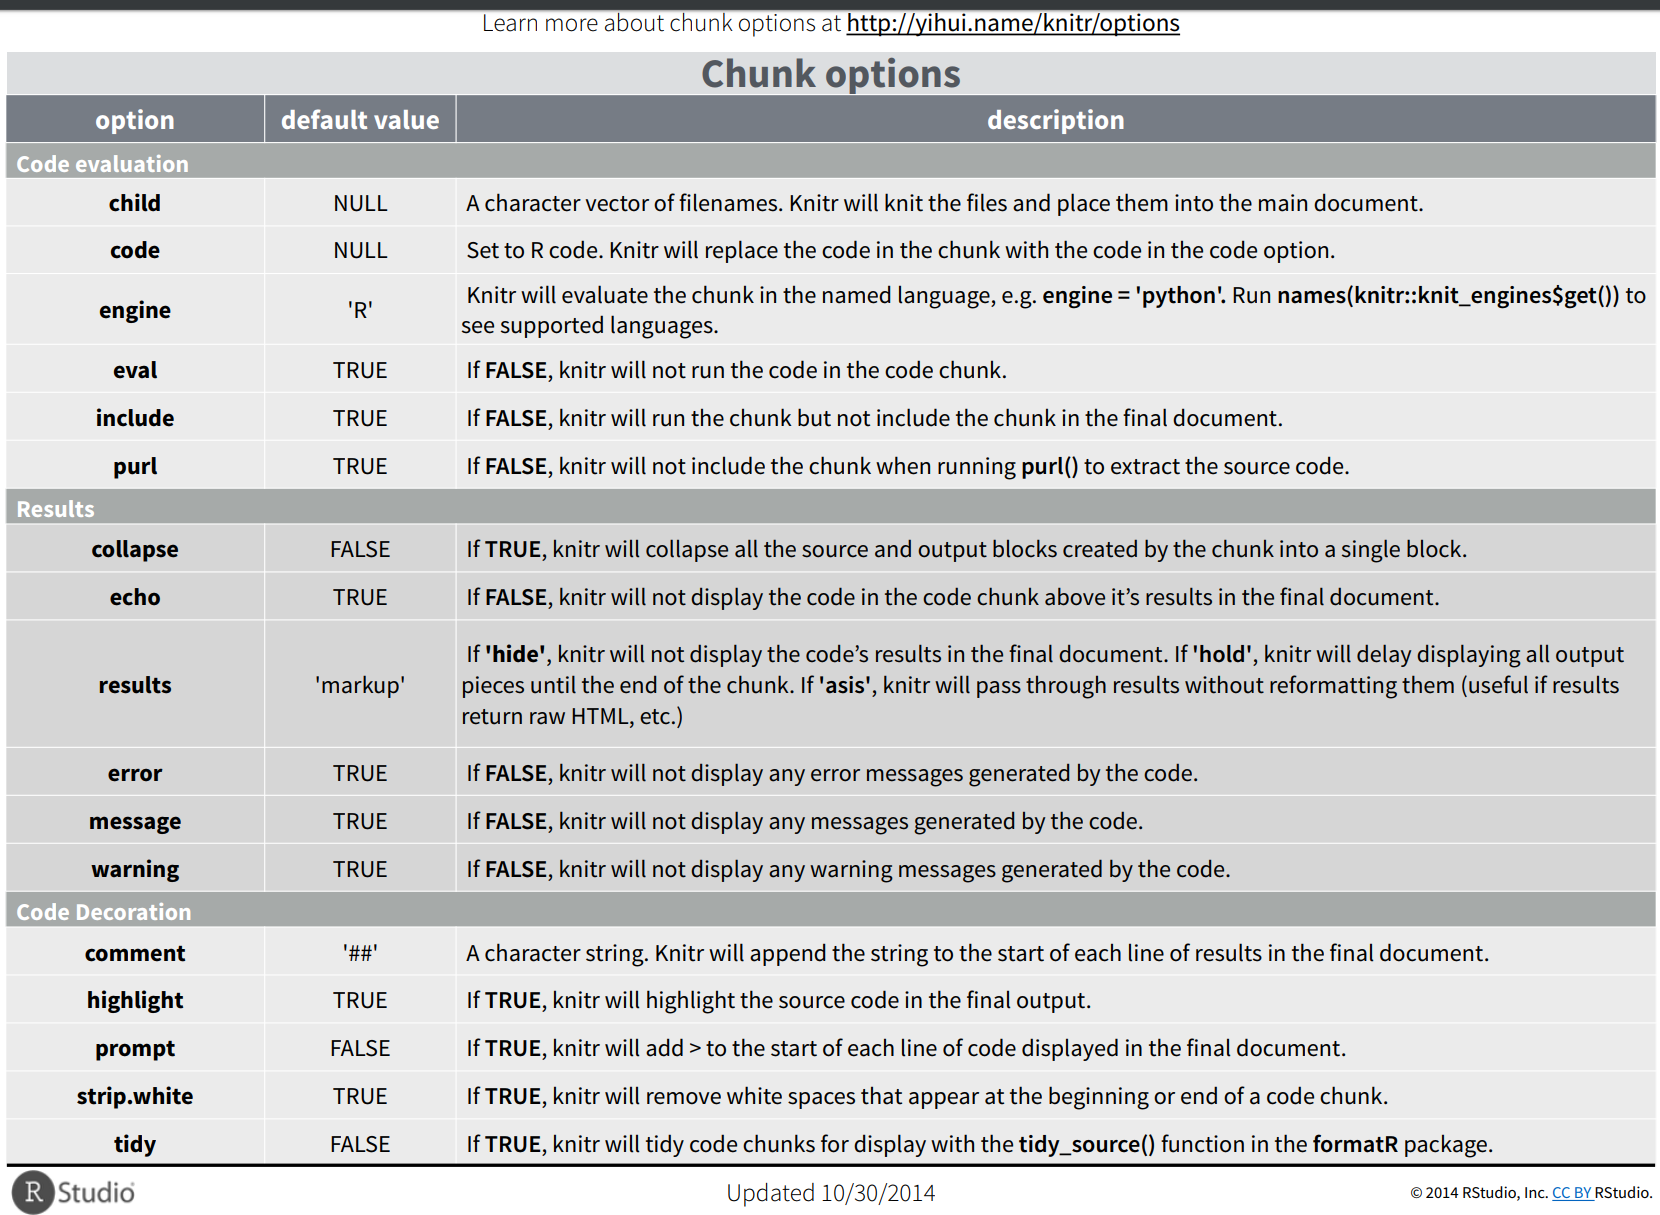
\includegraphics[width=\textwidth, keepaspectratio]{img/rr/knitropts.png}
\caption[knitr options]{A schematic table of options available using knitr and rmarkdown packages.}
\label{fig:knitropts}
\end{figure}


\subsubsection{Class Methods}

The class is provided of several methods for \textit{rmarkdown} \gls{cc} construction.

Once an \textit{easyReporting} instance is available, with \lstinline!mkdTitle! it is possible to insert six levels of titles, by setting the parameters \lstinline!title! and \lstinline!level!.
It is also possible to add natural language comments with \lstinline!mkdGeneralMsg!.

When working with \glspl{cc}, two main choices are available.
The first one gives the possibility to construct a \gls{cc} as additional steps, by using first the \lstinline!mkdCodeChunkSt!, then adding variable assignment and/or function calling with \lstinline!mkdVariableAssignment! or \lstinline!mkdGeneralMsg!, and finally closing the \gls{cc} with \lstinline!mkdCodeChunkEnd!.

In particular, when starting a \gls{cc} with \lstinline!mkdCodeChunkSt!, it is possible to assign a specific \lstinline!optionList! and/or a \lstinline!source.files.list! to be added to that \gls{cc}.

Otherwise it is possible to create an entire \gls{cc} just with \lstinline!mkdCodeChunkComplete! and assigning the entire function call as a \lstinline!message!.
This way of working is really useful with \lstinline!function! creation, where inside a developed function a simple recursive call with parameters assignment can be done as a single \lstinline!message!.





\subsection{Peak Caller} \label{sec:descan2peakcall}
However, the package can work with any external peak caller returning results in terms of bed files, indeed the package provides additional functionalities to load bed files of peaks and handle them as GenomicRanges \cite{Lawrence2013} structures.

\subsection{Peak Filtering and Alignment} \label{sec:descan2filtering}

In order to filter out false positives peaks, we designed a method (\lstinline{finalRegions}) which firstly filters out low score regions and then aligns the resulting regions between the samples, using two different thresholds.
One on the peaks's score and one on the number of samples.

The filtering step is designed to take as input a list of peaks as \textit{GenomicRangesList}, where each element represents a file.
This is the data structure produced by the peak caller, but, we also developed a method to load peaks produced by other software like MACS \cite{Zhang2008}, as described in section \ref{sec:descan2addfeat}.

Firstly, using the threshold on the peaks's score (\lstinline{zThreshold} parameter), the method filters out the peaks with a score lower than the user-defined threshold value.

Then, for aligning the peaks between the samples, it extends a 200bp window in both directions of remaining regions, computing the overlaps using the \lstinline{findOverlapsOfPeaks} method (with \lstinline{connectedPeaks} parameter set as \lstinline{merge}), as defined in \textit{ChIPpeakAnno} \cite{Zhu2010} R/Bioconductor package.

Based on this idea, the filtering step is developed to filter out those peaks not present in at least a user-defined (\lstinline{minCarriers} parameter) number of samples. In the light of this, the user can decide the minimum number of samples where each peak has to be detected.
On our experience, we suggest to set the samples threshold as a mutiple of the number of replicates of the conditions.


\subsection{Counting Peaks} \label{sec:descan2peakcounts}
The counting step (\lstinline{countFinalRegions} method) is designed to take a \textit{GenomicRanges} data structure as input, where for each peak additional features, as the score and the number of samples, are saved.
Moreover, it requires also the path of the BAM/BED files where the reads are stored, in order to quantify the peaks given as input.

For each region the method counts the number of reads present in each sample.
In so doing, it produces as result a matrix of the counts, where the rows and the columns represent, respectively, the regions and the samples.

In order to keep trace of all information associated to the regions, it produces a \textit{SummarizedExperiment} \cite{SummExp} data structure, giving the possibility to retrieve the \textit{GenomicRanges} peaks associated data structure and the count matrix, respectively, with \lstinline{rowRanges} and \lstinline{assays} method.

The choice to produce a count matrix is guided by the versatility of this data structure, useful not only for the differential enrichment of the regions between multiple conditions, but also for integrating the epigenomic data with other -omics.
\subsection{Additional Features} \label{sec:descan2addfeat}
The package offers additional features for loading data (i.e. peaks) resulting from other sources, and for manipulating \textit{GenomicRanges} data structure.

The method \lstinline{readFilesAsGRangesList} takes as input a directory with BAM or BED data, to load in \textit{GenomicRangesList} format.
This data structure is useful to store genomic information, as peaks or mapped reads, produced by other software like \textit{MACS2} or \textit{STAR} and, in case of peaks, it is necessary during the \gls{descan} filtering step.
Additionally to \lstinline{fileType} (BAM, BED, BED.zip) parameter specification it requires the genome code to use during the file processing.
Moreover, when the input files represent peaks the \lstinline{arePeaks} flag needs to be set to \lstinline{TRUE}.
In such a way the \gls{descan} package can work also with data coming from other sources, preferred by the user.

Furthermore, \gls{descan} provides several functionalities for GenomicRanges data structure
handling. One over the others (\lstinline{fromSamplesToChrsGRangesList}) gives the possibility to split a GenomicRangesList by the chromosomes. 
This procedure could be useful for parallelizing the computations on the chromosomes, assigning a single chromosome to a single computing unit.
Taken as input a GenomicRangesList organized by samples, this method returns a list of chromosomes, where each element has a GenomicRangesList of samples, containing only the regions associated to the single chromosome.

[Create figure to better explain the transformation]

Other useful utilities are \lstinline{keepRelevantChrs}, that takes a GenomicRangesList and a list of chromosomes and return only the interested chromosomes.
\lstinline{saveGRangesAsTsv} that saves a tab separated value file starting from a GenomicRanges.
\lstinline{saveGRangesAsBed} that save a standard BED file format starting from a GenomicRanges data structure.
\lstinline{setGRangesGenomeInfo} which, starting from a genome code, sets a specific \textit{genomeInfo} to a \textit{GenomicRanges} object.
\section{Case Study} \label{sec:descan2results}
\textbf{Few words on ATAC-Seq data}

We illustrate the performances of \gls{descan} using a dataset \cite{Su2017} that describes in vivo adult mouse dentate granule neurons before and after synchronous neuronal activation using Atac-Seq and RNA-Seq technologies (see sections \ref{sec:atacseq} and \ref{sec:rnaseq} for a description of these sequencing techniques).

This dataset is organized in 62 samples of Atac-Seq and RNA-Seq, extracted at different time points, with four replicates at each time point.
We chose to compare the differences btween the first two stages, time 0 (E0) and 1 hour after neuronal induction (E1), in order to show a possible Atac-Sec workflow for Differential Enrichment, and how to integrate this data type with RNA-Seq. A general illustration of our dataset is represented in figure \ref{fig:atacdataset}.

\begin{figure}[H]
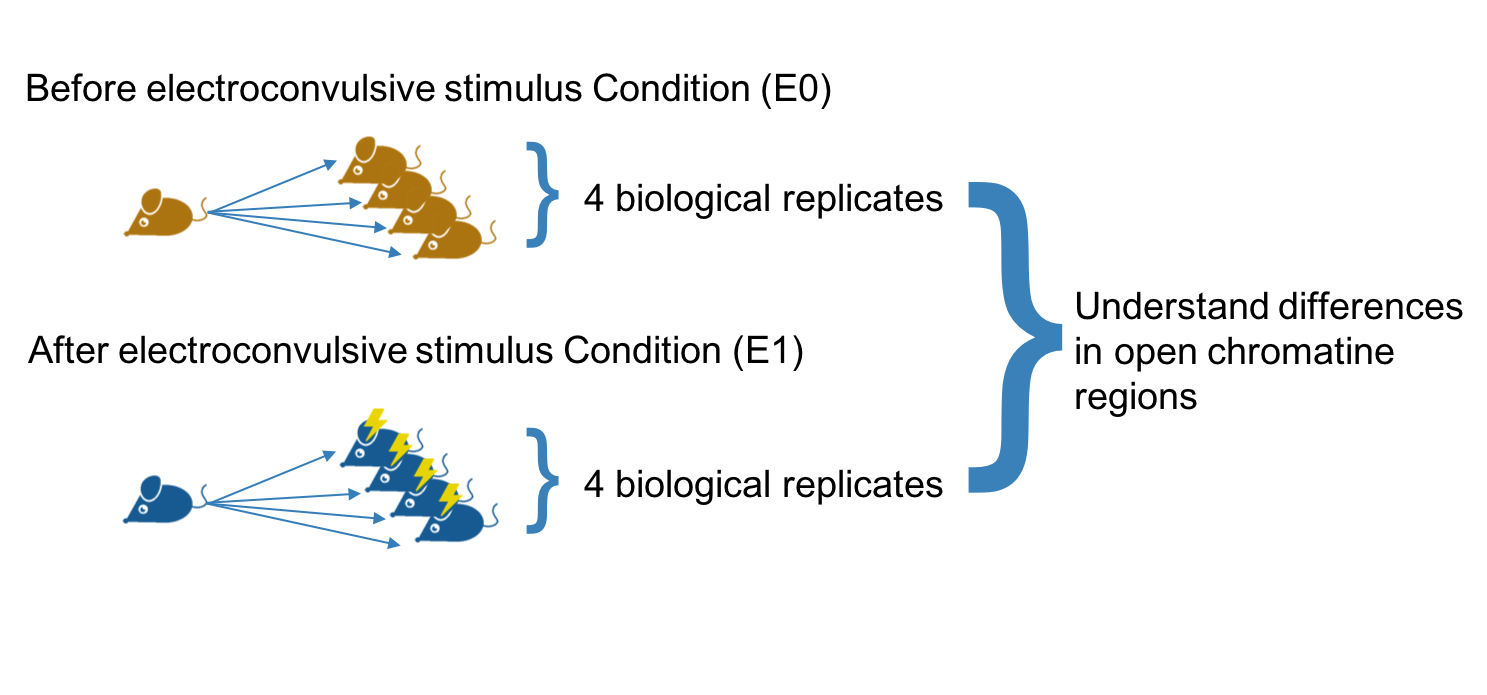
\includegraphics[width=\textwidth,height=\textheight,keepaspectratio]{img/descan2/dataset.png}
\caption[DEScan2 dataset illustration]{An illustration of our extraction of the \cite{Su2017} dataset.}
\label{fig:atacdataset}
\centering
\end{figure}

We downloaded the data from \gls{geo} database \cite{Edgar2002, Barrett2013} with accession number GSE82015\footnote{\url{https://www.ncbi.nlm.nih.gov/geo/query/acc.cgi?acc=GSE82015}} and mapped raw data using \textit{STAR} \cite{Dobin2013} with default parameter on \gls{mm10}.

In order to detect the open chromatin regions we run our peak caller, cutting the genome in bins of 50bp and using running windows of minimum 50bp and maximum 1000bp. In such a way we are able to detect not just broad peak, but also smaller peaks.

To be confident with our results we compared the \gls{descan} detected peaks with the same validated regions (Arc and Gabrr1) in the original work \cite{Su2017}.
The lower part of figure \ref{fig:peaksdescan} shows the detected and validated regions (in blue and red) resulting differentially enriched between the E0 (in pink) and E1 (in green) conditions, while the upper part shows \gls{descan} peaks (in blue), highlighting a capability to catch not only the same regions of the published ones, but also (gold circles) to be more careful in the smaller peaks detection.

\begin{figure}[H]
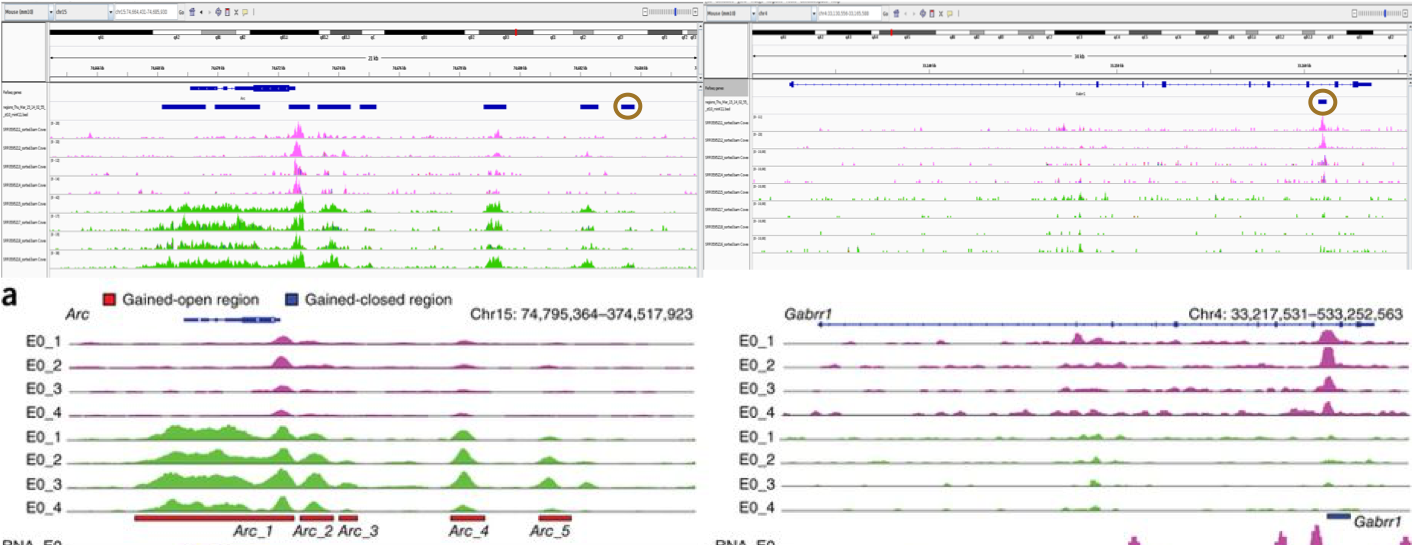
\includegraphics[width=\textwidth,height=\textheight,keepaspectratio]{img/descan2/peaks.png}
\caption[\gls{descan} peaks detection]{A comparison of \gls{descan} detected peaks with validated peaks in article \cite{Su2017}.}
\label{fig:peaksdescan}
\centering
\end{figure}

Moreover, we run \textit{MACS2} on the same samples, and (as shown in figure \ref{fig:des2m2peaks}) \gls{descan} seems able to catch much more peaks than \textit{MACS2} for each sample.

\begin{figure}[H]
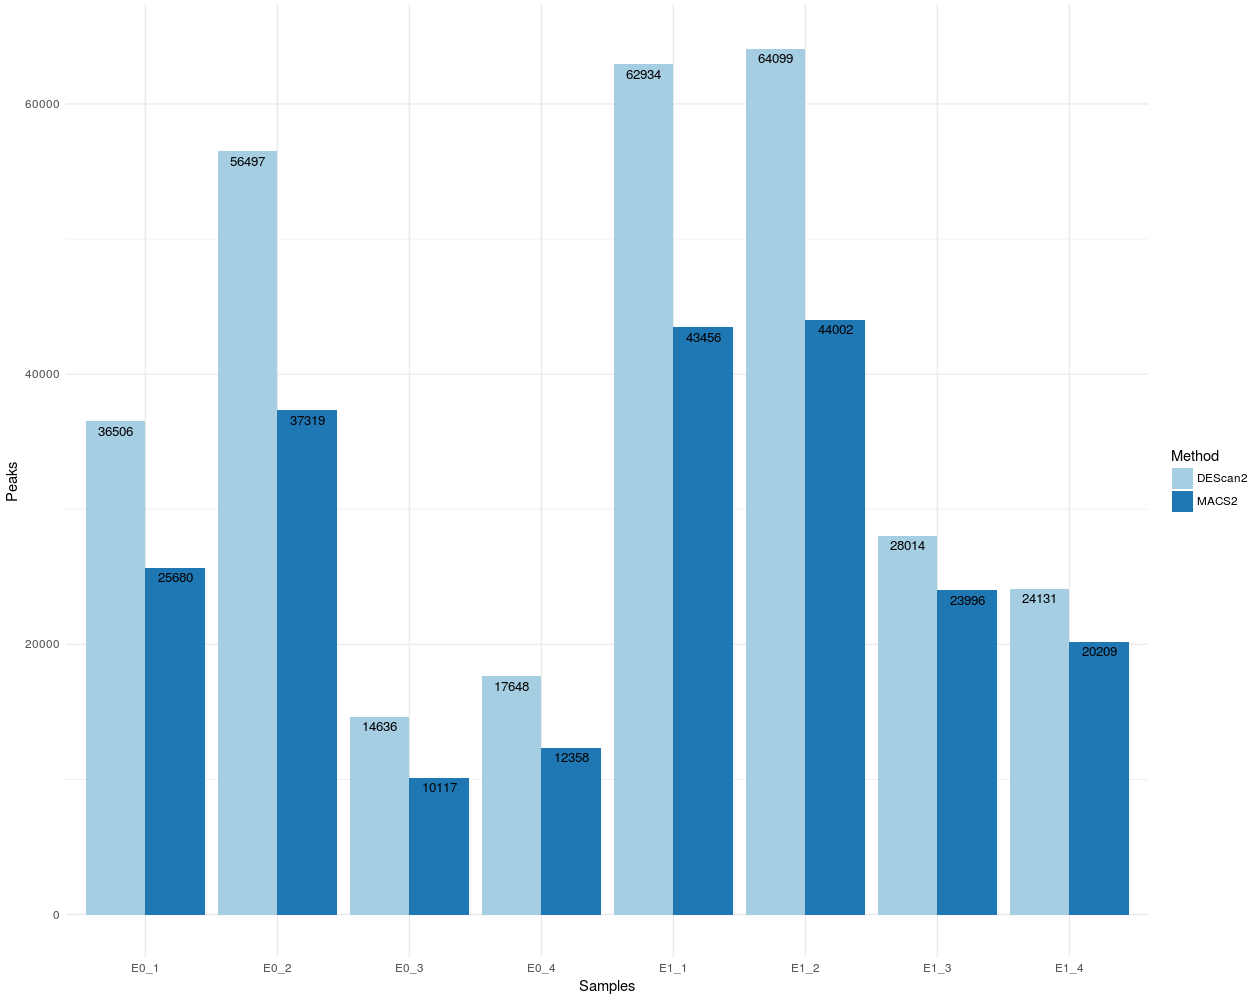
\includegraphics[width=\textwidth,height=\textheight,keepaspectratio]{img/descan2/d2m2_peaks_number.png}
\caption[The \gls{descan} and \textit{MACS2} peaks detection]{A comparison of \gls{descan} and \textit{MACS2} detected peaks for each sample in the dataset.}
\label{fig:des2m2peaks}
\centering
\end{figure}

While it is very important to detect good peaks with a peak caller, it seems to be more relevant to detect reliable regions. Indeed, during the filtering step, the number of peaks depends not only by the peak score, but also by the number of replicates designed in the experiment.
The figure \ref{fig:filteringdescan} puts in relation these two relevant information. 
On the x-axis is represented the number of replicates, while on the y-axis is traced the number of peaks, and each curve represents a different threshold on the peaks score, showing that higher are the thresholds on the scores and the number of replicates, lower is the number of the detected peaks.
Highlighting a proportional inversion between the number of the peaks and the combination of the number of samples and the detected regions score.


\begin{figure}[H]
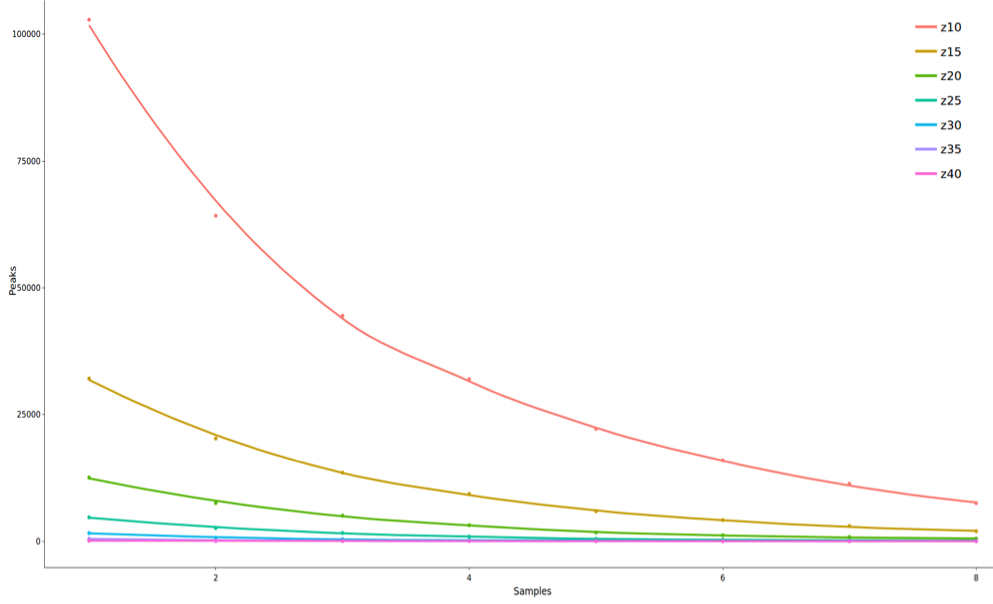
\includegraphics[width=\textwidth, height=\textheight, keepaspectratio]{img/descan2/filtering.png}
\caption[\gls{descan} filtering step]{Filtering the detected regions with different thresholds on peak scores.}
\label{fig:filteringdescan}
\centering
\end{figure}


\begin{figure}[H]
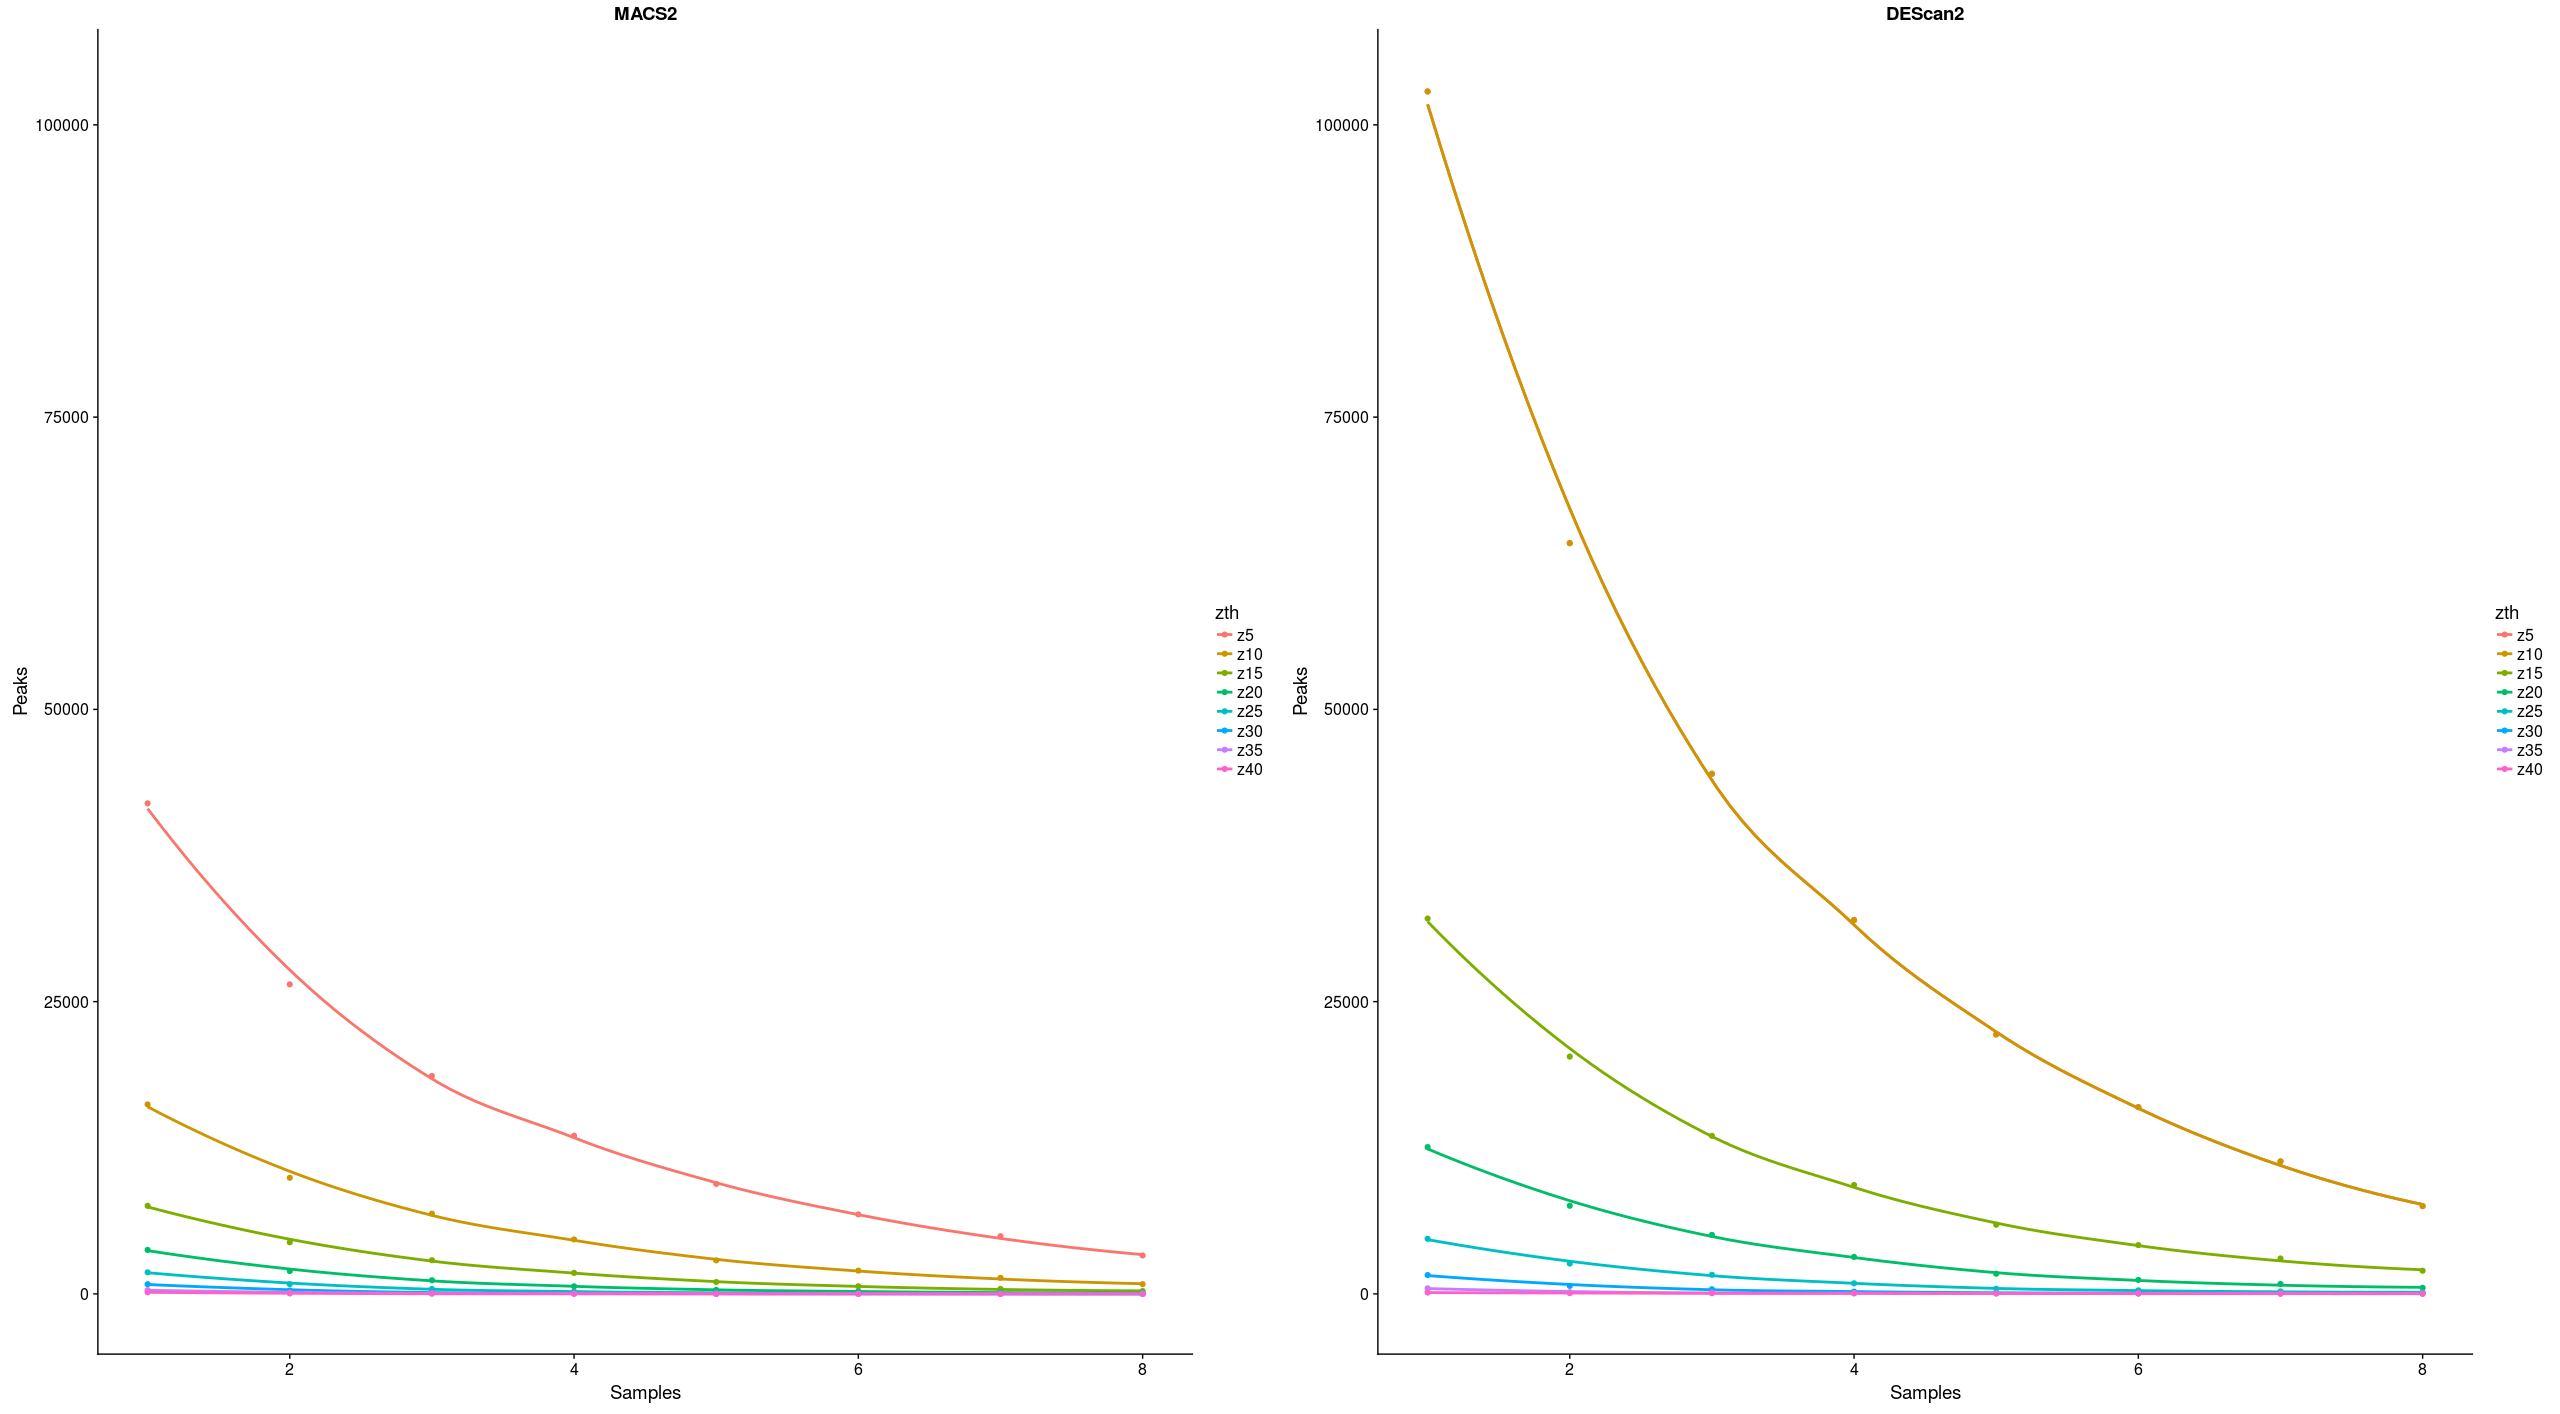
\includegraphics[width=\textwidth, height=\textheight, keepaspectratio]{img/descan2/filtering_m2_d2.png}
\caption[\gls{descan} and \textit{MACS2} filtering comparison]{Filtering the detected regions with different thresholds on peak scores between \textit{MACS2} and \gls{descan}.}
\label{fig:filteringdescanmacs2}
\centering
\end{figure}

The filtered-in regions can be processed by \gls{descan} in order to obtain a count matrix with samples on the columns and peaks on the rows.
This type of data structure is very versatile, because it enables to perform several operations, like the \glspl{der} and, if possible, the integration with other kind of omics, as RNA-Seq.

In order to preserve the information associated to the peaks, \gls{descan} produces as output a \textit{SummarizedExperiment} (figure \ref{fig:countsdescan}) data structure, which enables to retrieve the count matrix with \lstinline{assays} method, and to access the peaks information in \textit{GenomicRanges} format with the \lstinline{rowRanges} method. %{

\begin{figure}[H]
\centering
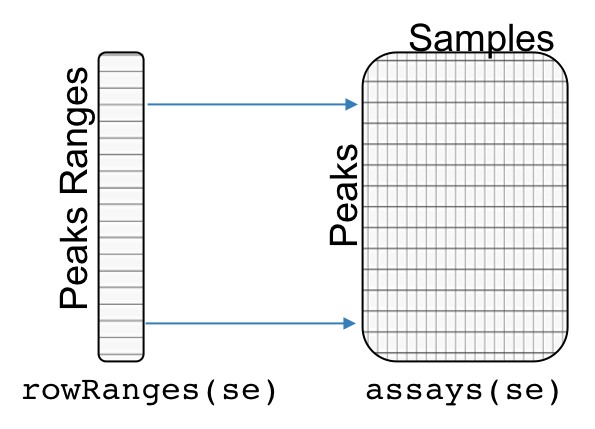
\includegraphics[keepaspectratio]{img/descan2/counts.png}
\caption[\gls{descan} counts illustration]{An illustration of the \textit{SummarizedExperiment} data structure produced by \gls{descan}.}
\label{fig:countsdescan}
\centering
\end{figure}

Before to proceed to detect \glspl{der}, it is a good standard to normalize the data, also because without any kind of normalization we are not able to detect any \gls{der}.
The nature of the data, in count format, makes it possible to apply several well known RNA-Seq normalizations techniques, as \textit{TMM}, \textit{upper-quartile}, \textit{full-quantile}, \textit{RUV-Seq}, etc \cite{Risso2014, Robinson2010, Dillies2013}.

While the \textit{TMM} and \textit{upper-quartile} normalizations modify the data in a way that makes it impossible to detect \glspl{der}, other kind of normalizations and combinantions of them give good results.

The figure \ref{fig:normalizationsdescan} sintetizes this concept very well, highlighting a relation between the number of \glspl{der} and the minumum number of samples used for filtering the data during the \gls{descan} filtering step.

The plot shows that \textit{upper-quantile}, even if combined with \textit{RUV-Seq} normalization, is not able to linearly detect a good amount of \glspl{der}, while \textit{full-quantile}, when combined with \textit{RUV-Seq} seems to affect the data in a way that overdetect the number of \glspl{der}. 
When looking at the \textit{full-quantile} and \textit{RUV-Seq} by themself seem to perform better than the other normalizations. The first one has a downhill almost linear, while the second one has a very fast downhill with a regrowth when the number of samples is higher.

Even if these normalization methods show good performances with this type of epignomic data, our investigations suggest that more testing is required, but maybe an ad-hoc normalization method for these data has to be developed.

\begin{figure}[H]
\centering
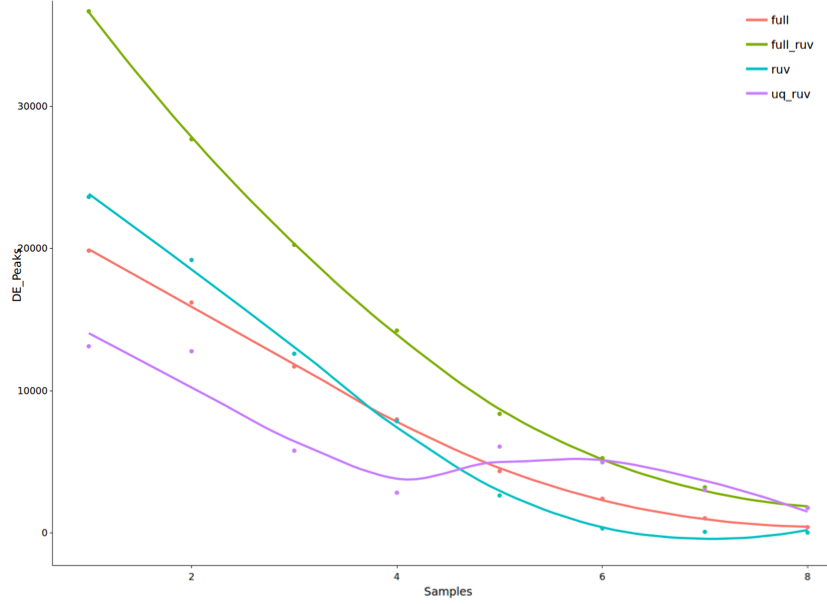
\includegraphics[width=\textwidth, height=\textheight, keepaspectratio]{img/descan2/normalizations.png}
\caption[Normalizations applied to detected regions]{The figure shows the effects of different normalizations on the epigenomic differentially enriched regions.}
\label{fig:normalizationsdescan}
\centering
\end{figure}

To estimate the \glspl{der}, any of the RNA-Seq methods can be applied, such as \textit{DESeq2}, \textit{edgeR}, \textit{NOISeq}, etc \cite{Robinson2009, McCarthy2012, Tarazona2012}.

In this case, we decided to use \textit{edgeR} package, because of its wide range of  available statistical approaches and the possibility to better tune the design of the experiment. 
Indeed, because we used the RUV-Seq normalized counts with \lstinline{k} parameter set to 4, we modeled the experimental design with the \lstinline{model.matrix} function, adding to our model not only the experimental conditions, but also the RUV-Seq estimated weights.
Then we used the resulted design to estimate the dispersion and fit a Quasi-Likelihood test, as defined in edgeR.

The figure \ref{fig:depeaksdescan} shows a volcano plot of \glspl{der} between E0 and E1 conditions.
Red dots highlights the regions with a False Discovery Rate (FDR) lower than 0.05, while blue dots highlight not significant regions.
 
\begin{figure}[h]
\centering
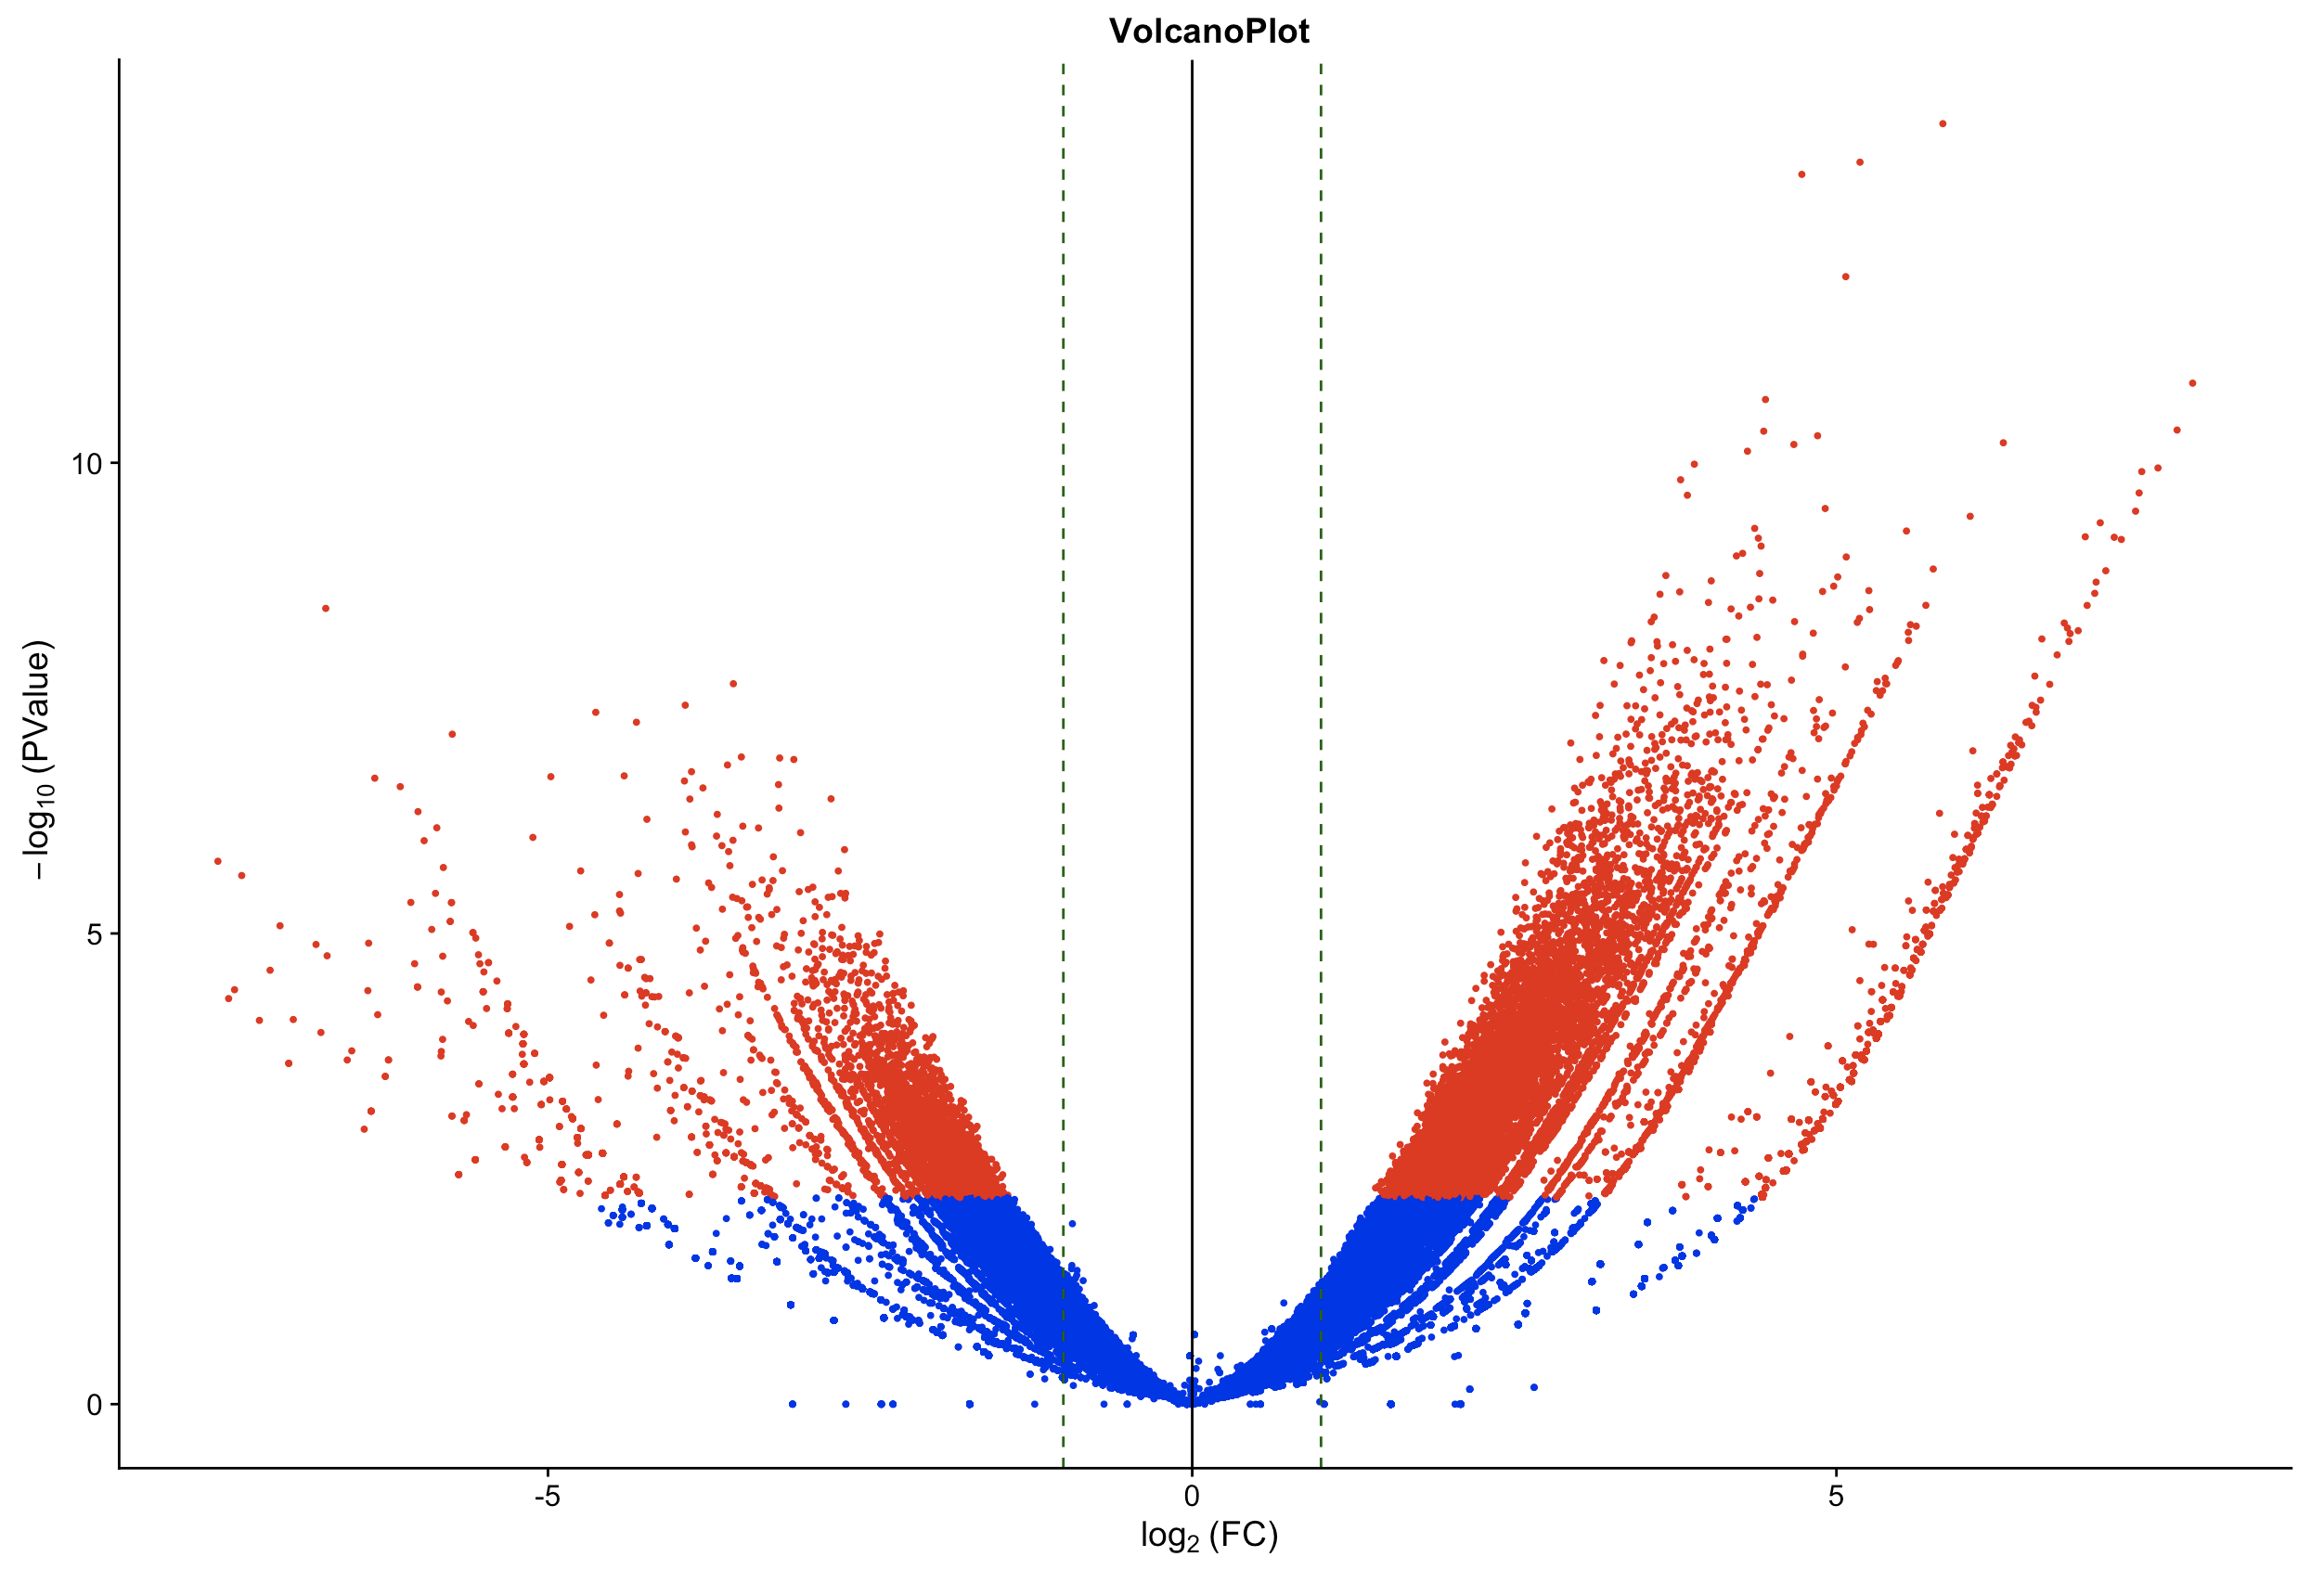
\includegraphics[width=\textwidth, height=\textheight, keepaspectratio]{img/descan2/DE_peaks.png}
\caption[Differential Enrichment Regions Volcano]{A volcano plot of Differential Enriched Regions. Blue dots represent the not significant \glspl{der}, while the red ones represent the significant \glspl{der}.}
\label{fig:depeaksdescan}
\centering
\end{figure}

Next task is to integrate the obtained results with other omic data types, as RNA-Seq. 
Because of the low number of the samples, the easiest way to integrate the data is to annotate the \glspl{der} with differentially expressed genes resulting from the analysis of RNA-Seq.

For the Differential expression of the RNA-Seq data we firstly quantified the signal with \lstinline{featureCounts} methods available in the \textit{Rsubread} \cite{Liao2013} Bioconductor package.
Then we filtered lowly expressed genes with the \textit{proportion} test  as implemented in \textit{NOISeq} package, and applied the \lstinline{noiseq} method for differential expression.%{

\begin{figure}[h]
\centering
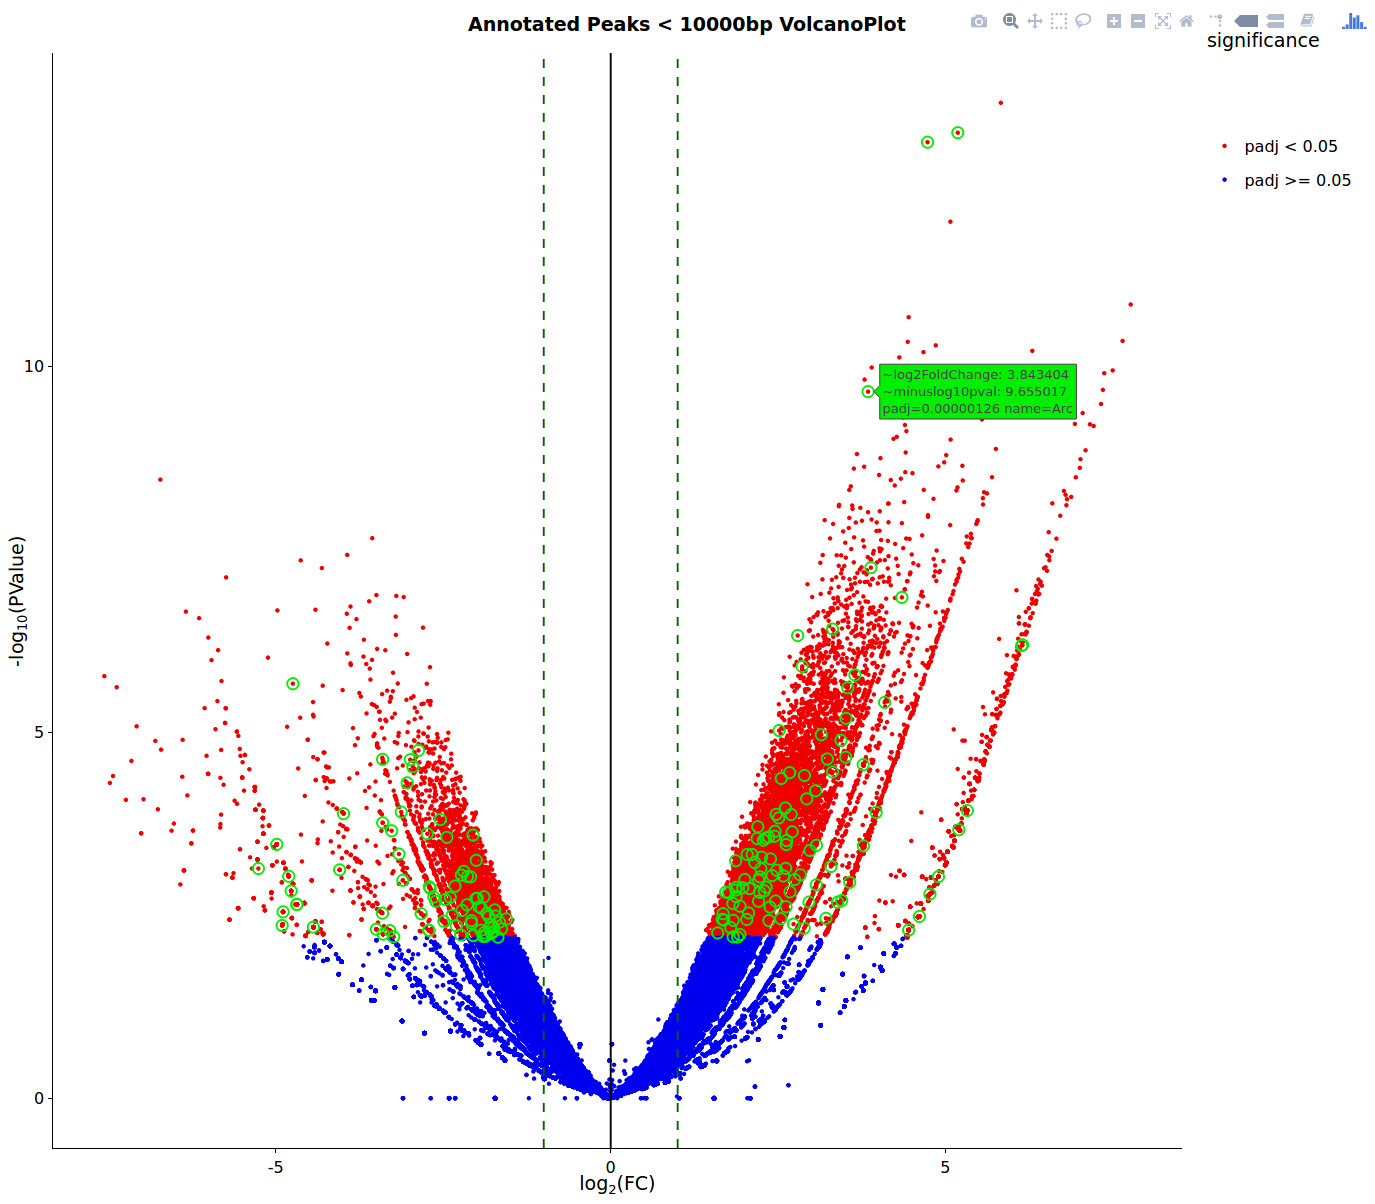
\includegraphics[width=\textwidth, height=\textheight, keepaspectratio]{img/descan2/Annotated_depeaks_degenes.png}
\caption[Annotated Differential Enrichment Regions Volcano]{A volcano plot of \glspl{der}. Blue dots represent the not significant \glspl{der}, while the red ones represent the significant \glspl{der}. Green circles highlights the peaks with a \gls{deg} annotated.}
\label{fig:depeakdegenessdescan}
\centering
\end{figure}

We selected the significant \glspl{deg} with a probability higher than 0.95, and used these genes to annotate the peaks with \lstinline{annotatePeakInBatch} method of ChIPpeakAnno.
Figure 	\ref{fig:depeakdegenessdescan} illustrates with green circles the peaks with an annotated gene with distance lower than 10000bp from the gene TSS.
Realizing the plot with the \textit{plotly} library it's possible to enhance the names of the genes with a tip window.










\section{Discussions} \label{sec:descan2next}
Multiple omics data information extraction became always more complex with the evolution of sequencing techniques and with the consequent development of methodologies for their analysis and integration.
With this thesis work, we focused on the development of novel strategies for several problems related to multiple omics sequencing data information extraction.

Firstly, we approached the most studied genomic problem, transcriptomic, by focusing on time-course \textit{RNA-seq} data.
We presented \textit{ticorser}, an R command line package for time-course \textit{RNA-seq} data.
With this instrument we propose a complete pipeline for the time-course data analysis, presenting also ad-hoc designed approaches for this type of data visualization at different levels.
Additionally, allowing a first integration level with functional annotation and also for their visualization.

Afterwards, we focused on \textit{ATAC-seq} technology, an emerging technique for open chromatin region detection, which still needs appropriate solutions for its analysis.
To address the lack of methodologies with this data we presented \textit{DEScan2}, an R/Bioconductor package allowing detection of open chromatin regions, and proposed a possible workflow for the detection of \glspl{der} and their integration with \textit{RNA-seq} data.

Due to the difficulty of keeping track even a single omic analysis, we presented \textit{easyReporting}, a possible approach to the Reproducible Research inside R.
A tool which helps not only software developers to include \gls{rr} layers inside their tools, but also non-expert R analysts to easily produce reports for their analysis.

Finally, to speed up and help also non-expert users to analyze multiple omics data, we presented \gls{igro}, a web graphical user interface for the analysis of omics data.
Combining the flexibility of a point-and-click approach with the power of R/Bioconductor statistical approaches for the omics data analysis.
Moreover, thanks to the Reproducible Research layer it allows to keep track of all the steps performed during the analysis, and with aid of dedicated interface to live edit the enriched report.

%%%%%%%%%%%%%%%%%%%%%%%%%%%%%%%%%%%%%%%%%%%%%%%%%%%%%%%

\chapter{A reproducible research tool: the R6 Class easyReporting}
%As previously mentioned in section \ref{sec:reprres}, in the omics data field, the complexity of the analysis, due to the data high-dimensionality and to the wide range of methodologies to use, has revived an interest in \gls{rr}, because of the difficulties in reproducing third-party scientific findings.

%Basically, the implementation of the \gls{rr} is pretty complex, requiring a combination of multiple tools, each one with a different final scope.

%In this Chapter we illustrate \textit{easyReporting} a novel R package for speeding up the \gls{rr} implementation when analyzing data or when constructing other packages.

It has been claimed that many research findings in omics science are false (or partially false) due to accidental mistakes or mis-usage of methods.
To prevent misleading results it is important to be able to inspect and reproduce the entire data analysis carried out in a unified product.

\gls{rr} consists on making available both the analytic data and the associated code in a manner that other researchers might reproduce the findings. 

In this Chapter we illustrate \textit{easyReporting} a novel R package for speeding up the \gls{rr} implementation when analyzing data or when constructing other packages.

Tool availability at: \url{https://github.com/drighelli/easyreporting}
\section{The idea of Reproducible Research}
In order to deeply understand and reconstruct cellular mechanisms influenced by drug treatments, pathologies or diseases, it is fundamental to look at multiple omics data types at the same time.

Previous chapters deeply described tools for multiple omics data analysis, integration and visualization using command line tools.
Even if the command line approach is pretty common inside the bioinformatics community, it is not for every scientist who is not so confident with programming languages or terminal.
When working with multiple omics data, there is an overabundance of available tools for each sequencing that can bewilder a beginner, up to the point to renounce approaching the analysis problem.

%Moreover, thanks to our previous experiences \cite{russo2015advantages} in developing \gls{gui}, we noticed a growing interest by the scientific community in using interactive software.
%This interest seems to be leaded by multiple motivations, such as the need to analyze data very fast or the lack of time in learning programming languages and terminal-line based tools.

Furthermore, even if the bioinformatics community has massively moved on the development of novel statistical and computational methods for multi-omics data integration, part of the scientific community is still anchored to the single-omics analysis side.
Even if still really helpful, it is still very common to read published papers based on single-omics data analysis without taking into account possible integrated solution with other omics data types.

Of course, it is not so simple to afford for multiple omics data experiments, but, nowadays, the internet swarms of public datasets.
In particular when looking at public biological data banks, such as \gls{geo}\footnote{\url{https://www.ncbi.nlm.nih.gov/geo/}} \cite{Services2007} or \gls{tcga}\footnote{\url{https://cancergenome.nih.gov/}} \cite{tcga2013a}, where it is possible to retrieve as many data as needed.

On the other side, if there are not so many papers publishing integrated analysis, it is also difficult for analysts to retrieve the right methodologies for the multi-omics data analysis and their visualization. 

\begin{figure}[H]
\centering
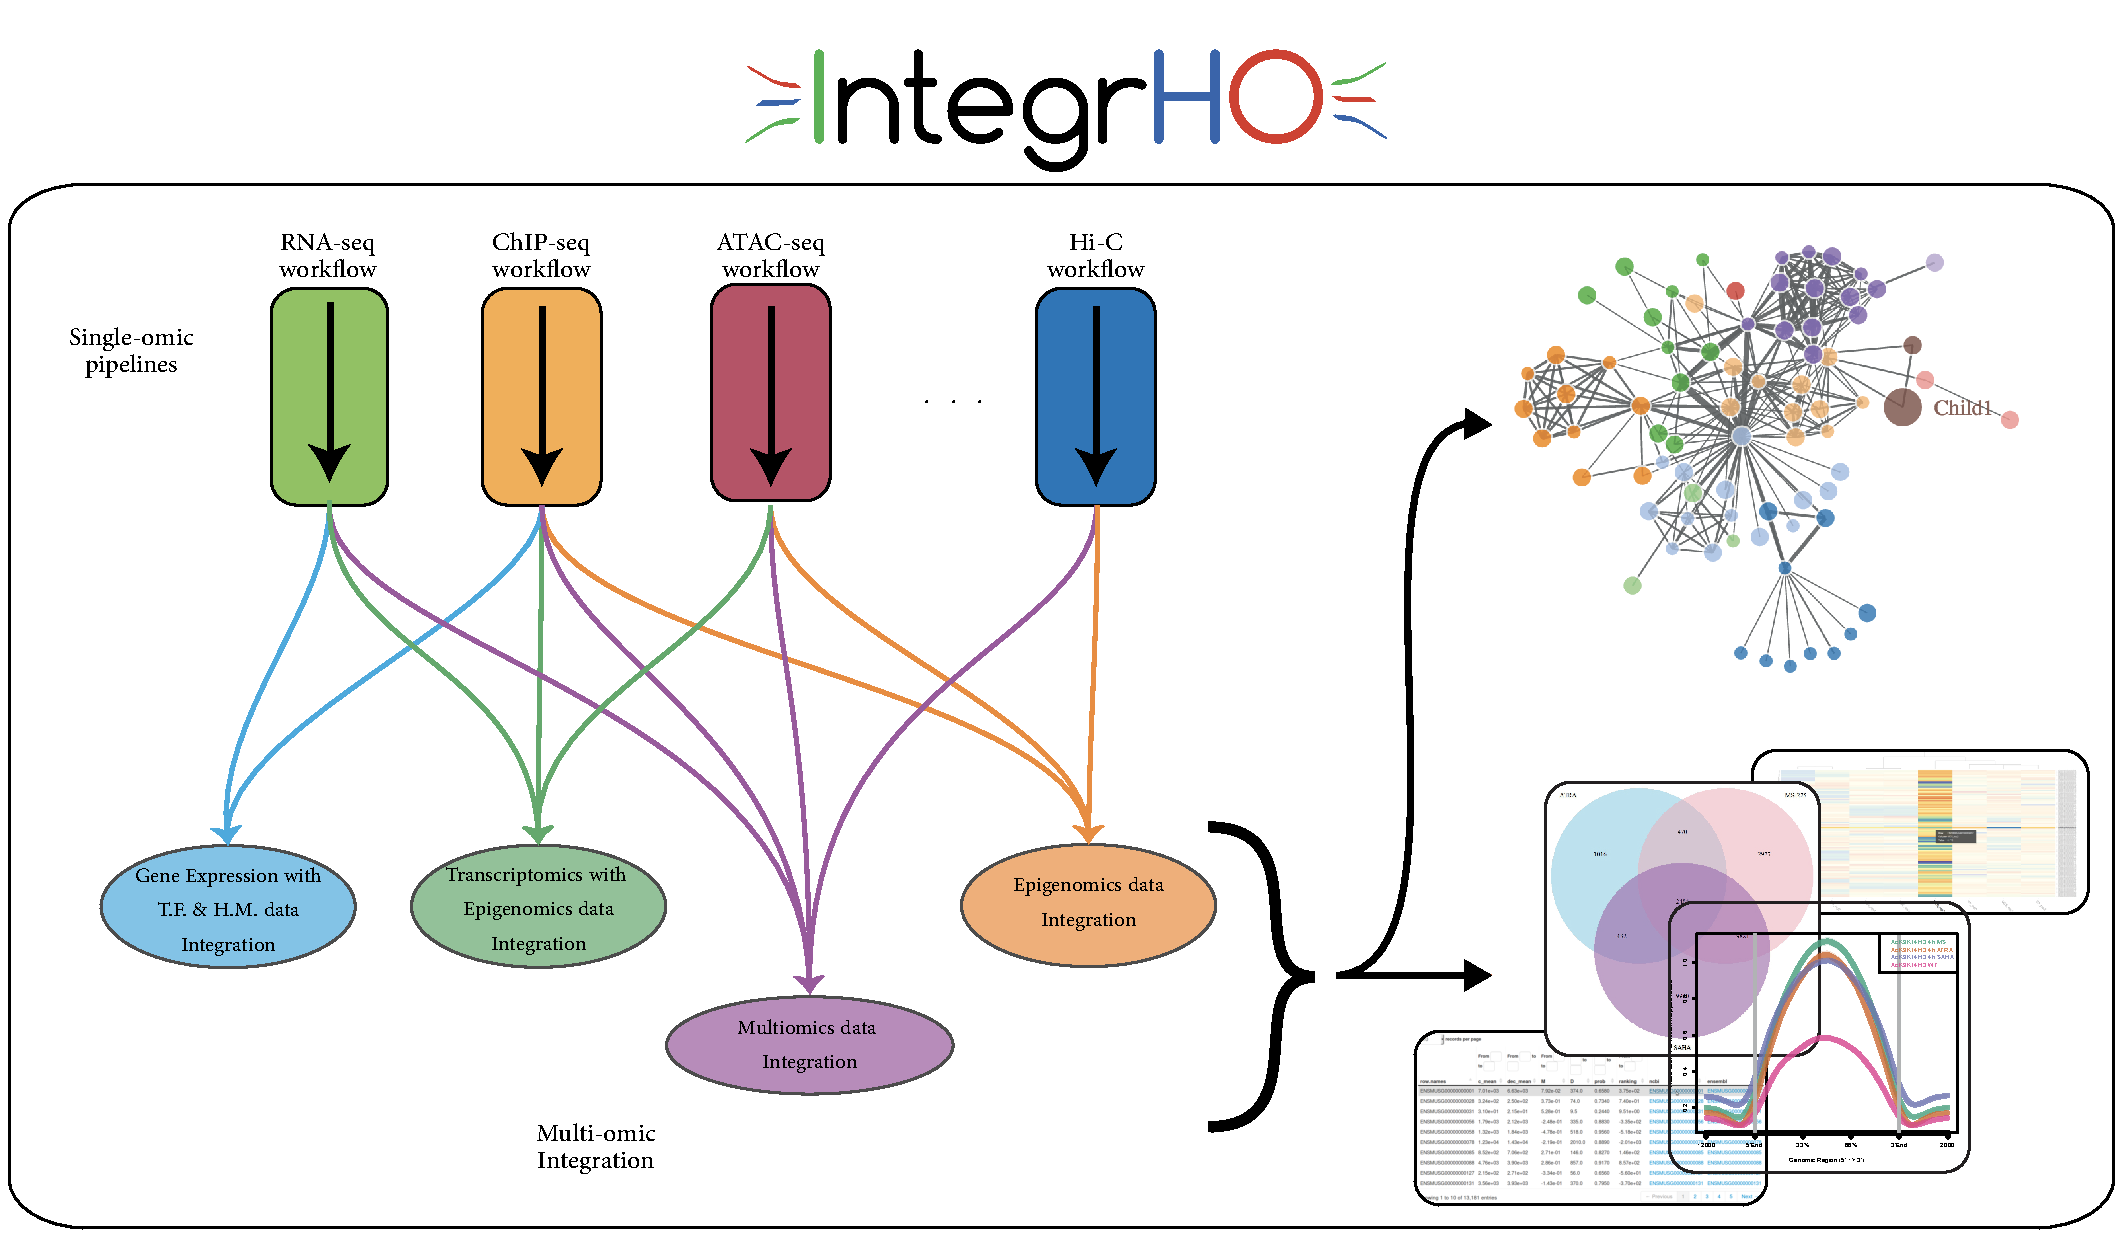
\includegraphics[width=\textwidth, keepaspectratio]{img/integrho/integrho_scheme.pdf}
\caption[\gls{igro} representation]{A schematical representation of \gls{igro} underlying idea.
Single-omics analysis methods are proposed in order to facilitate their multiple integration.
This integration can lead to produce graphical results, in case of low dimension datasets, or to more sophisticated integration model such as regulation networks, in case of high-dimension datasets.}
\label{fig:integrhoidea}
\end{figure}

Based on these considerations and in order to promote the multi-omics data integration, we decided to provide the scientific community of a novel easy-to-use instrument which not only gives the possibility to analyze single-omics data types but also guides the user through multiple ways of integrating multi-omics data types (figure \ref{fig:integrhoidea} gives an underlying idea of \gls{igro}).





%Several interface-based tools \cite{Poplawski2016} have been proposed during last years but too often they are oriented to analyze singular-omics or when designed for multi-omics, they are pipeline oriented. 

%In this chapter we introduce \gls{igro}, our web-based platform for multi-omics data analysis and integration,  in a \gls{rr} spirit.



\section{Methods}
Here we present \textit{easyReporting}, an \textit{R6} \footnote{\url{https://adv-r.hadley.nz/r6.html}}\footnote{\url{https://cran.r-project.org/web/packages/R6/index.html}} class\footnote{\url{https://en.wikipedia.org/wiki/Class_(computer_programming)}} developers to integrate a reproducible research layer inside their software products, as well as lazy analysts to speed up their report production without learning the \textit{rmarkdown} language.

In such a way, thanks to minimal additional efforts of developers, the end user has available an \textit{rmarkdown} file within all the source code generated during the analysis, divided into \glspl{cc} ready for the compilation.

Once manually edited with comments and descriptions the file can be compiled to produce an enriched document within input data, source code and output results.

A so final document can be attached to the publication of the analysis as supplementary material, helping the interested community to entirely reproduce the computational part of work (figure \ref{fig:rrscheme}). 

The package is accessible at the following link:\\ \href{https://github.com/drighelli/easyreporting}{https://github.com/drighelli/easyreporting} 

\subsubsection{General Description and Initialization}

The class can to be imagined as a schematic representation of the \textit{rmarkdown} file (\textit{report}), indeed 
its attributes represent the \textit{report} characteristics, which are typically inserted in the header of the file.
But our class methods are not only for the attributes manipulations but also for insertion of \glspl{cc}, comments and section titles inside the \textit{report}.

As any typical class, before of using it, \textit{easyReporting} requires to be initialized with the \lstinline!new! command, passing as mandatory arguments the \textit{path} and the name of the file as \lstinline!filenamepath! and a title as \lstinline!mainTitle!.
Additionally, an \lstinline!author! and the \lstinline!documentType! can be specified.

When initializing, the class automatically creates the \textit{report} with the entire specified folder tree, setting up the header of it and declaring the general options for the \textit{rmarkdown} file.
If \textit{rmarkdown} personal options (see figure \ref{fig:knitropts} for a list of available options) are required, before creating an instance of the class, it is possible to use the \lstinline!makeOptionsList! function, and then assigning the output to the \lstinline!optionsList! argument of the class \lstinline!constructor!.

\begin{figure}[H]
\centering
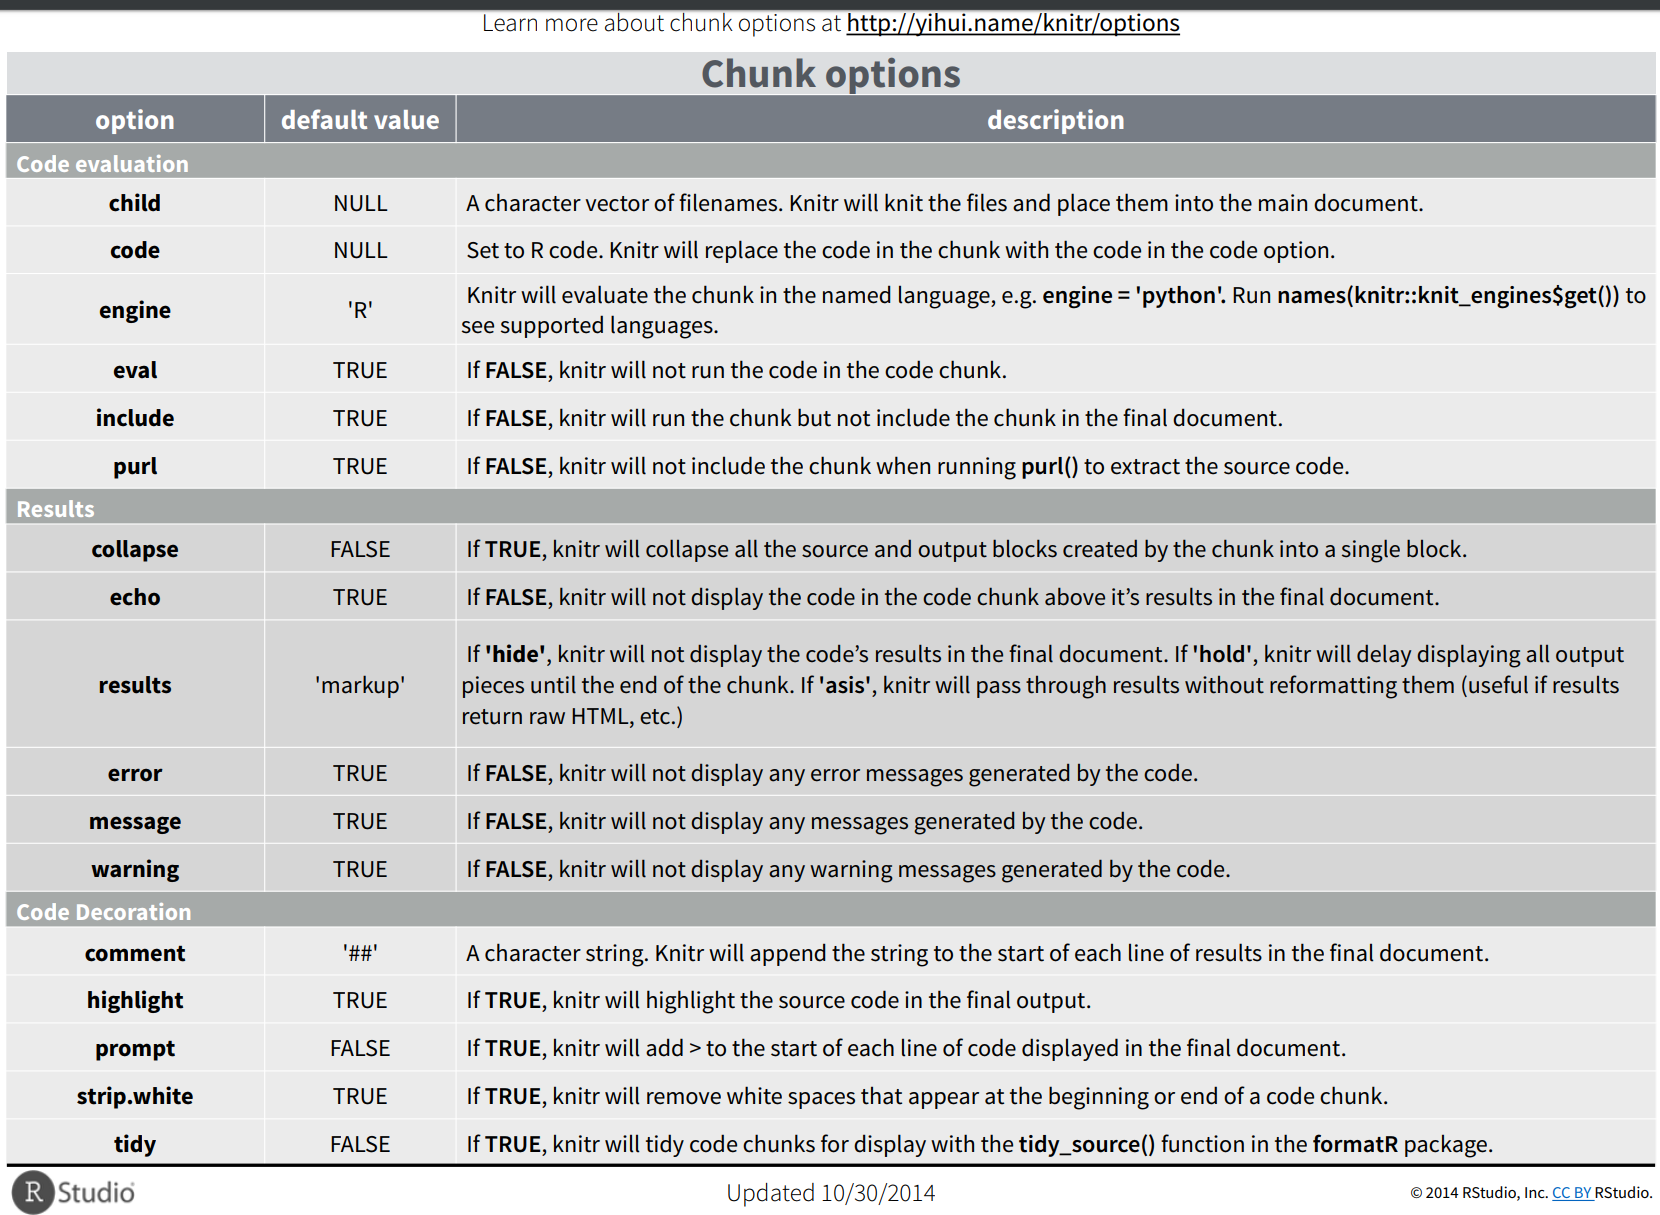
\includegraphics[width=\textwidth, keepaspectratio]{img/rr/knitropts.png}
\caption[knitr options]{A schematic table of options available using knitr and rmarkdown packages.}
\label{fig:knitropts}
\end{figure}


\subsubsection{Class Methods}

The class is provided of several methods for \textit{rmarkdown} \gls{cc} construction.

Once an \textit{easyReporting} instance is available, with \lstinline!mkdTitle! it is possible to insert six levels of titles, by setting the parameters \lstinline!title! and \lstinline!level!.
It is also possible to add natural language comments with \lstinline!mkdGeneralMsg!.

When working with \glspl{cc}, two main choices are available.
The first one gives the possibility to construct a \gls{cc} as additional steps, by using first the \lstinline!mkdCodeChunkSt!, then adding variable assignment and/or function calling with \lstinline!mkdVariableAssignment! or \lstinline!mkdGeneralMsg!, and finally closing the \gls{cc} with \lstinline!mkdCodeChunkEnd!.

In particular, when starting a \gls{cc} with \lstinline!mkdCodeChunkSt!, it is possible to assign a specific \lstinline!optionList! and/or a \lstinline!source.files.list! to be added to that \gls{cc}.

Otherwise it is possible to create an entire \gls{cc} just with \lstinline!mkdCodeChunkComplete! and assigning the entire function call as a \lstinline!message!.
This way of working is really useful with \lstinline!function! creation, where inside a developed function a simple recursive call with parameters assignment can be done as a single \lstinline!message!.





\section{Usage}
Here we report an example script where a general illustration of the \textit{easyReporting} is described.

As already mentioned, the class allows to report not only the \gls{cc}, but also to add personal titles and personal comments, enhancing the knowledge transfer between the ''back-side'' (the analyst/developer) and the ''front-side'' (the reader) users.
Note that ''back-side'' and ''front-side'' can also be the data analyst and the collaborators, respectively.
\\
\begin{lstlisting}
## Creating report file with default options on global document
rd <- easyreporting$new(filenamepath="./project_report", title="example_report", author=c("Dario Righelli"))

rd$mkdTitle("First Level Title")

rd$mkdGeneralMsg("Here I'm writing a simple paragraph useful to describe my code chunk")

## Leaving the default options to the code chunk
rd$mkdCodeChunkSt()

## Adding a variable assignement
variable <- 1
rd$mkdVariableAssignment("variable", "variable", show=TRUE)
rd$mkdCodeChunkEnd()

## Or i can create my own options for the chunk
rd$mkdTitle("Second Level Title", level=2)
optList <- maketOptionsList(includeFlag=TRUE)
rd$mkdCodeChunkSt(optionsList=optList)
rd$mkdCodeChunkEnd()

## Moreover I can add a list of files to source in che code chunk
rd$mkdCodeChunkSt(optionsList=optList, source.files.list=c("R/cachingFunctions.R", "R/cachingFunctions.R"))
rd$mkdCodeChunkEnd()

rd$mkdCodeChunkComplete(message="a <- 1\nb <- 2\nc <- a+b\n print(c)")

## Otherwise I can make a direct call with all the code chunk and the comment in one call
optList <- makeOptionsList(includeFlag=TRUE, cacheFlag=TRUE)

rd$mkdCodeChunkCommented(commentMsg="This is the comment of the following code chunk", message="a <- 1\nb <- 2\n(c <- a+b)", optionsList=optList, source.files.list=NULL)

## finally I can directly compile my report
rd$compile()
\end{lstlisting}

The previous R script leads to automatically produce the following rmarkdown file, where it is possible to see at rows 13 and 23 two titles at different levels.
And additionally, starting from row 15, a describing paragraph representing the additional comments that can be added to provide additional explanations to the following \gls{cc}.
\\

\begin{lstlisting}
---
    title: "example_report"
    author: "Dario Righelli"
    date: "`r Sys.Date()`"
    output: rmarkdown::html_document
---

```{r global_options, include=FALSE}
knitr::opts_chunk$set(eval=TRUE, echo=TRUE, warning=FALSE, message=FALSE, include=TRUE, cache=TRUE)
```

# First Level Title
Here I'm writing a simple paragraph useful to describe my code chunk

```{r eval=TRUE, echo=TRUE, warning=FALSE, message=FALSE, include=TRUE, cache=TRUE}
variable <- `variable`
print(variable)

```
## Second Level Title
```{r eval=TRUE, echo=TRUE, warning=FALSE, message=FALSE, include=TRUE, cache=TRUE}
```

```{r eval=TRUE, echo=TRUE, warning=FALSE, message=FALSE, include=TRUE, cache=TRUE}
source("/Users/inzirio/Desktop/gDrive/works/coding/easyreporting/R/cachingFunctions.R")
source("/Users/inzirio/Desktop/gDrive/works/coding/easyreporting/R/cachingFunctions.R")
```

```{r eval=TRUE, echo=TRUE, warning=FALSE, message=FALSE, include=TRUE, cache=TRUE}
a <- 1
b <- 2
c <- a+b
 print(c)
```

This is the comment of the following code chunk

```{r eval=TRUE, echo=TRUE, warning=FALSE, message=FALSE, include=TRUE, cache=TRUE}
a <- 1
b <- 2
(c <- a+b)
```
\end{lstlisting}

Thanks to the \lstinline!rd$compile()! command inside the first script, it automatically produces the final \gls{html} report illustrated in figure \ref{fig:rrreport}.

\begin{figure}[ht]
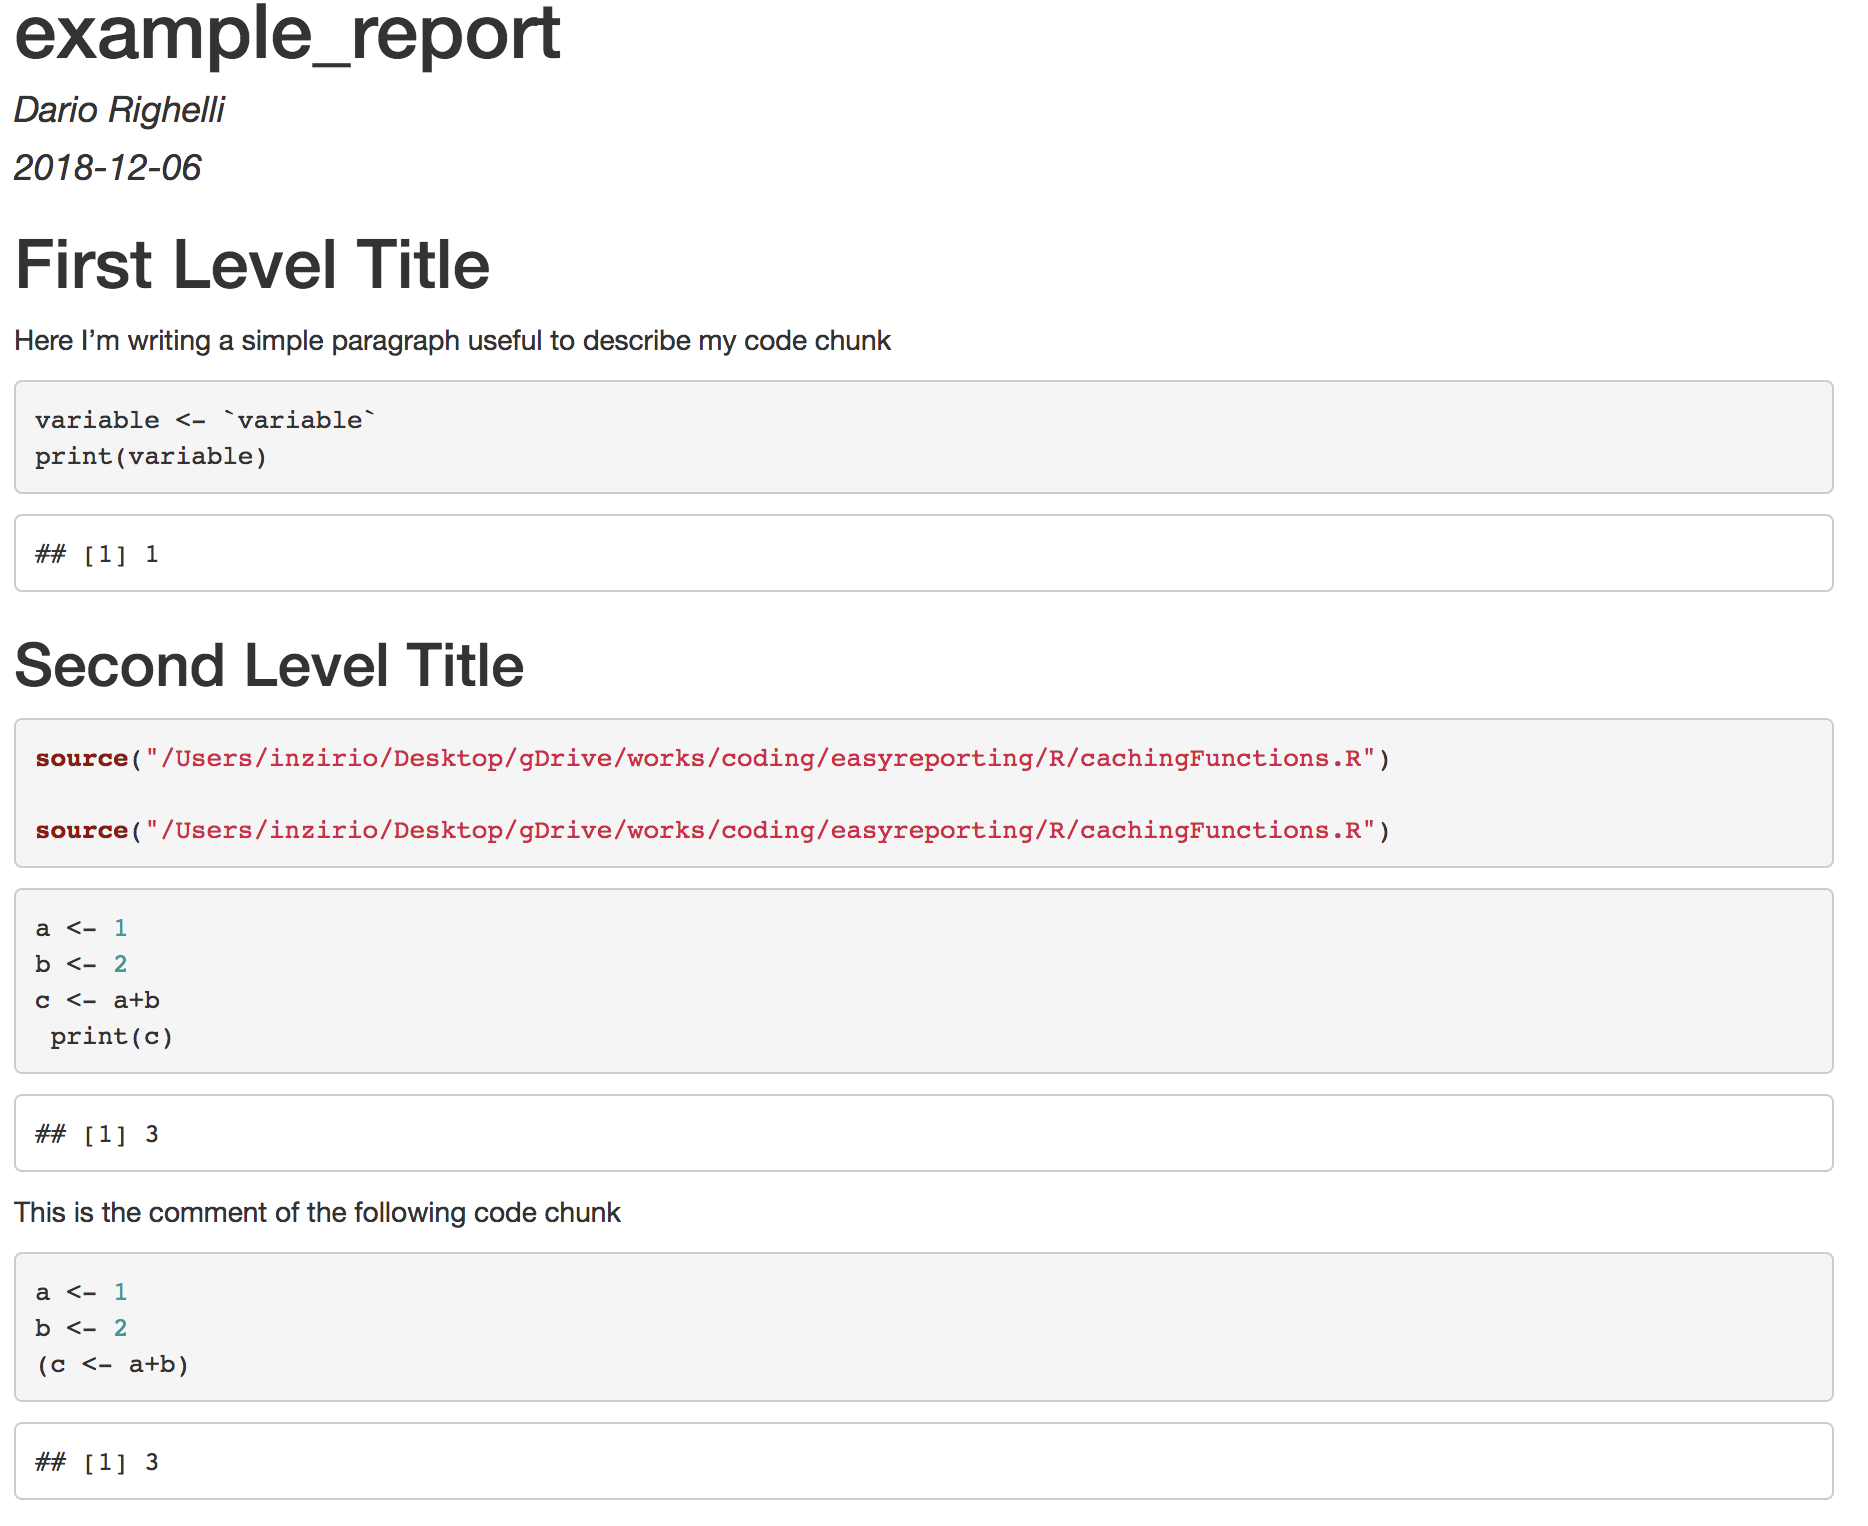
\includegraphics[width=\textwidth, keepaspectratio]{img/rr/report.png}
\caption[html report]{An example of HTML report produced with \textit{easyReporting} R package.}
\label{fig:rrreport}
\centering
\end{figure}

Finally, the report in \gls{html} format provides a human readable document, where all the \gls{cc} are highlithed in grey, and the results in white.
Titles and comments are in plain text, highlighting the natural language format of a self-explaining document.


\section{Discussions}
We presented \textit{easyReporting}, an R package enabling the implementation of \gls{rr} using rmarkdown language scripting, without any knowledge of it.

Despite other  previously proposed solutions \cite{Napolitano2013, Napolitano2017}, that always require too much commitment by the final user, potentially bringing him/her to totally renounce to include \gls{rr} inside the scripts, our approach is versatile and easy to be implemented, leaving maximum freedom to the final developer/analyzer, automatically creating and storing an \textit{rmarkdown} document, and providing also methods for its compilation.

It gives the possibility to obtain reproducible results and to publish better findings, increasing the scientific publications transparency by improving the knowledge transfer, and to support the methodologies integrity also into the scientific labs, where people can change position through the years.

On the other hand, the \textit{easyReporting} package, even if useful and easy to handle, can be improved with several additional functionalities.
While it is really important to generate an rmarkdown file, it could be useful to introduce methods for its file editing. 
Indeed, if an analyst or a final user, wants to correct an analysis, by changing an already inserted \gls{cc}, he/she could have the possibility to do this, by editing that specific \gls{cc} or by overwriting it.
A possible approach to do this could be to trace the \glspl{cc}, with a dedicated data structure, while inserting them, and give the possibility to the user to access them with specific class methods.

At the same time, even if the rmarkdown options enable the user to store the input/output data with \lstinline!cache! option, it could be better to provide caching methods, in order to give higher manageability of the data, storing them inside caching database files, as also reported in figure \ref{fig:rrscheme}.
Additionally, a caching store system (such as BiocFileCache\footnote{\url{https://bioconductor.org/packages/release/bioc/html/BiocFileCache.html}}) could produce caching database files, easily shareable through the Internet or as supplementary data of a publication.

In order to provide a graphical representation of an entire analysis, it could be useful to equip \textit{easyReporting} with methods for graph construction.
In such a way, the final report could be, not only read by third-party users, but also graphically impress the final reader.




%%%%%%%%%%%%%%%%%%%%%%%%%%%%%%%%%%%%%%%%%%%%%%%%%%%%%%%%%%%

\chapter{Integration of High-Throughtput Omics data: IntegrHO} \label{sec:integrhocap}

\textbf{\textsl{few words on integration of epigenomic with transcriptomic}}

To investigate and answer epigenetic biological questions we decided to create a useful instrument for analysing epigenomic data (such as \textit{ChIP-Seq}, \textit{Atac-Seq}, \textit{Sono-Seq}).
Very often the biological questions to be answered, as for the RNA-Seq, need the comparison of two or more different biological conditions.
Starting from a set of already published \cite{Koberstein2018} scripts, we designed \textit{Differential Enriched Scan 2} (\textit{DEScan2}), a software for helping the analysis of epigenomic data.
\section{Introduction} \label{sec:integrhointro}
In order to deeply understand and reconstruct cellular mechanisms influenced by drug treatments, pathologies or diseases, it is fundamental to look at multiple omics data types at the same time.

Previous chapters deeply described tools for multiple omics data analysis, integration and visualization using command line tools.
Even if the command line approach is pretty common inside the bioinformatics community, it is not for every scientist who is not so confident with programming languages or terminal.
When working with multiple omics data, there is an overabundance of available tools for each sequencing that can bewilder a beginner, up to the point to renounce approaching the analysis problem.

%Moreover, thanks to our previous experiences \cite{russo2015advantages} in developing \gls{gui}, we noticed a growing interest by the scientific community in using interactive software.
%This interest seems to be leaded by multiple motivations, such as the need to analyze data very fast or the lack of time in learning programming languages and terminal-line based tools.

Furthermore, even if the bioinformatics community has massively moved on the development of novel statistical and computational methods for multi-omics data integration, part of the scientific community is still anchored to the single-omics analysis side.
Even if still really helpful, it is still very common to read published papers based on single-omics data analysis without taking into account possible integrated solution with other omics data types.

Of course, it is not so simple to afford for multiple omics data experiments, but, nowadays, the internet swarms of public datasets.
In particular when looking at public biological data banks, such as \gls{geo}\footnote{\url{https://www.ncbi.nlm.nih.gov/geo/}} \cite{Services2007} or \gls{tcga}\footnote{\url{https://cancergenome.nih.gov/}} \cite{tcga2013a}, where it is possible to retrieve as many data as needed.

On the other side, if there are not so many papers publishing integrated analysis, it is also difficult for analysts to retrieve the right methodologies for the multi-omics data analysis and their visualization. 

\begin{figure}[H]
\centering
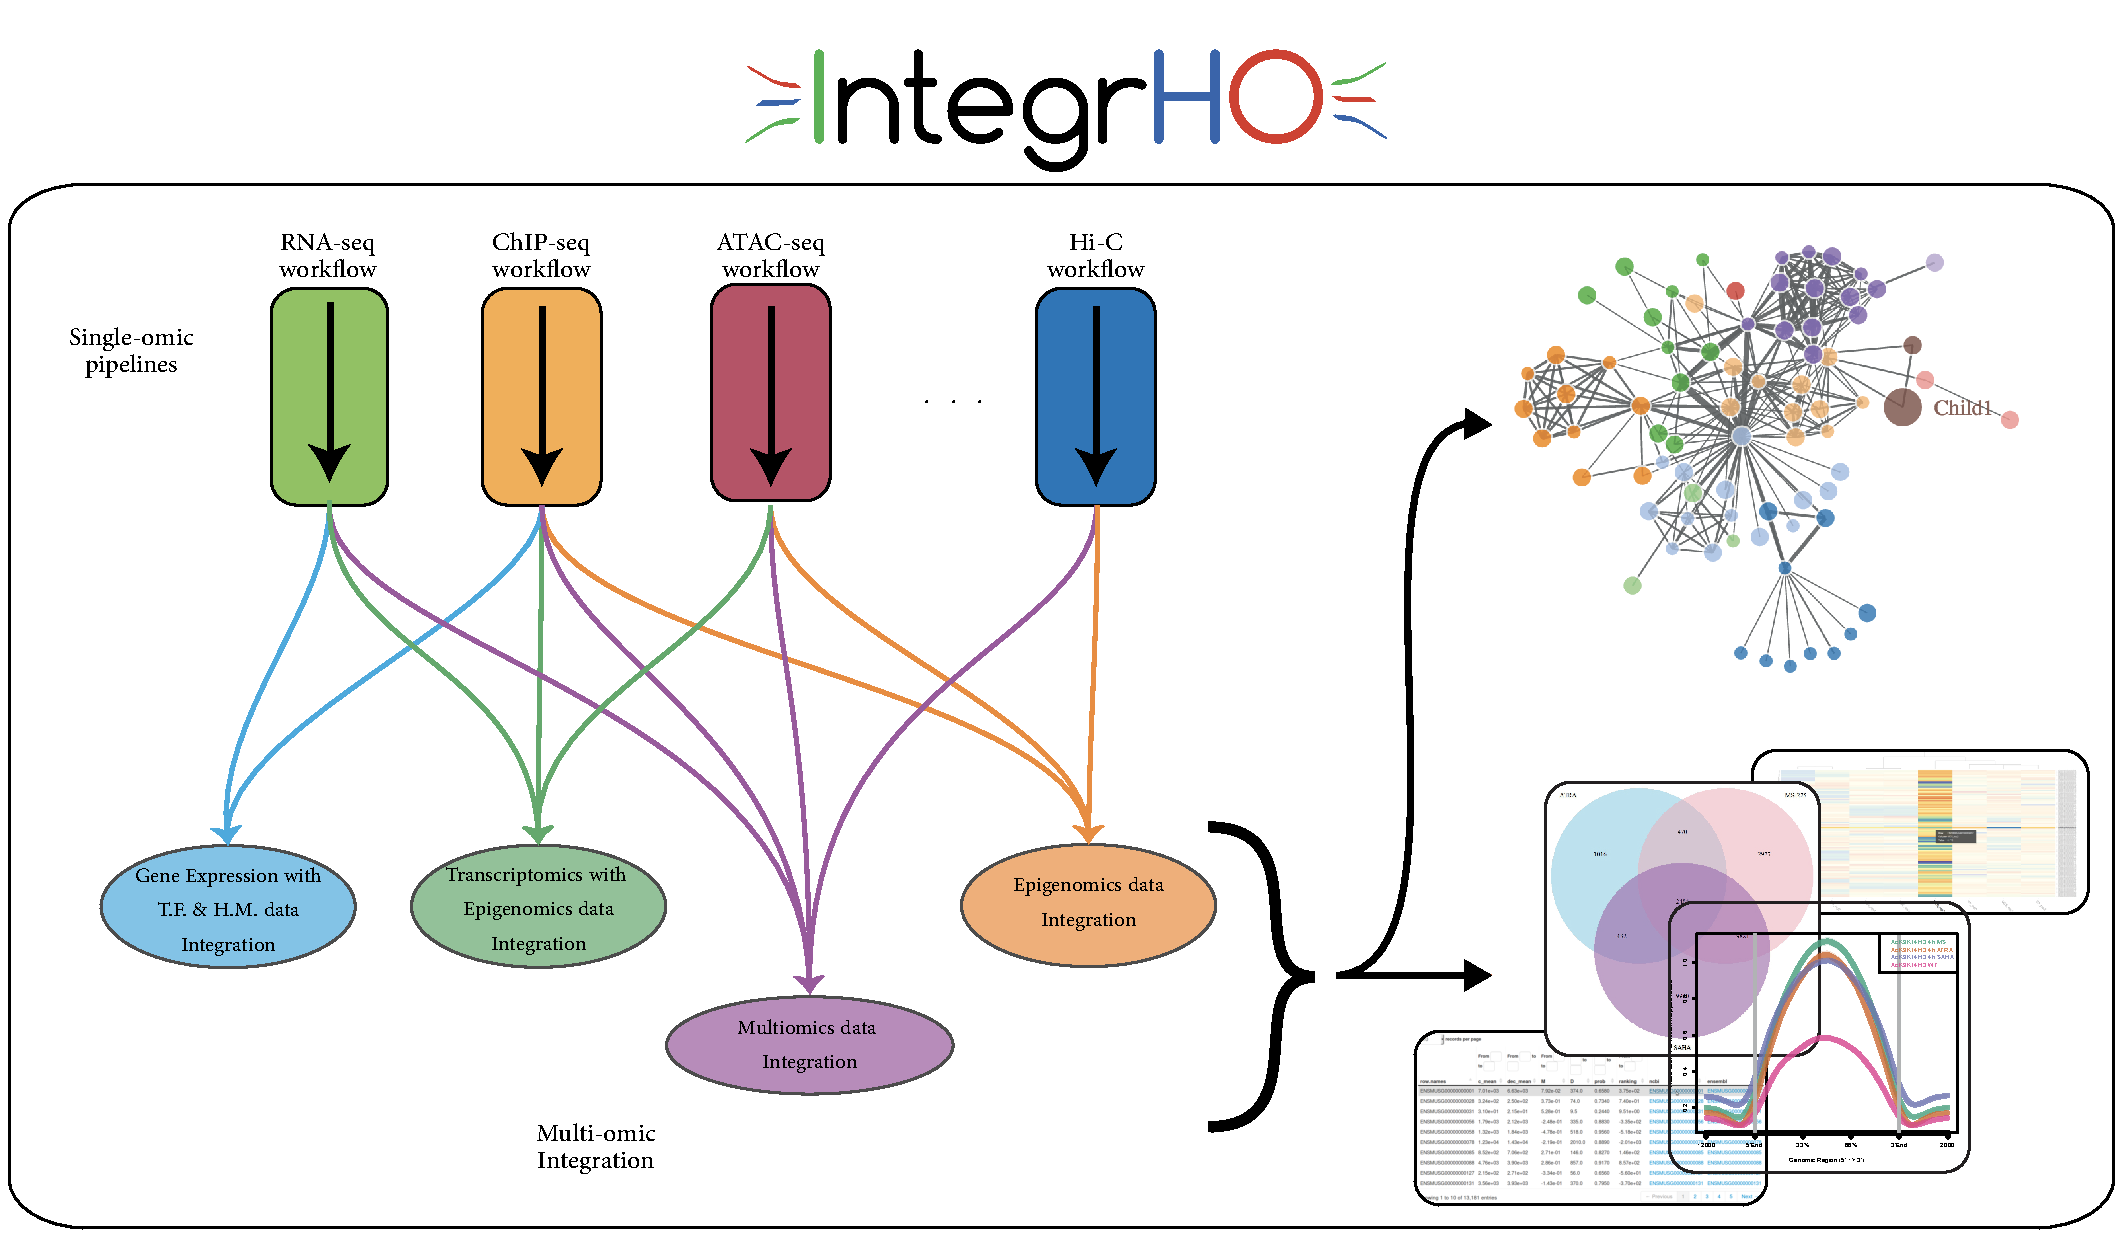
\includegraphics[width=\textwidth, keepaspectratio]{img/integrho/integrho_scheme.pdf}
\caption[\gls{igro} representation]{A schematical representation of \gls{igro} underlying idea.
Single-omics analysis methods are proposed in order to facilitate their multiple integration.
This integration can lead to produce graphical results, in case of low dimension datasets, or to more sophisticated integration model such as regulation networks, in case of high-dimension datasets.}
\label{fig:integrhoidea}
\end{figure}

Based on these considerations and in order to promote the multi-omics data integration, we decided to provide the scientific community of a novel easy-to-use instrument which not only gives the possibility to analyze single-omics data types but also guides the user through multiple ways of integrating multi-omics data types (figure \ref{fig:integrhoidea} gives an underlying idea of \gls{igro}).





%Several interface-based tools \cite{Poplawski2016} have been proposed during last years but too often they are oriented to analyze singular-omics or when designed for multi-omics, they are pipeline oriented. 

%In this chapter we introduce \gls{igro}, our web-based platform for multi-omics data analysis and integration,  in a \gls{rr} spirit.



\section{Methods}  \label{sec:integrhometh}
Here we present \textit{easyReporting}, an \textit{R6} \footnote{\url{https://adv-r.hadley.nz/r6.html}}\footnote{\url{https://cran.r-project.org/web/packages/R6/index.html}} class\footnote{\url{https://en.wikipedia.org/wiki/Class_(computer_programming)}} developers to integrate a reproducible research layer inside their software products, as well as lazy analysts to speed up their report production without learning the \textit{rmarkdown} language.

In such a way, thanks to minimal additional efforts of developers, the end user has available an \textit{rmarkdown} file within all the source code generated during the analysis, divided into \glspl{cc} ready for the compilation.

Once manually edited with comments and descriptions the file can be compiled to produce an enriched document within input data, source code and output results.

A so final document can be attached to the publication of the analysis as supplementary material, helping the interested community to entirely reproduce the computational part of work (figure \ref{fig:rrscheme}). 

The package is accessible at the following link:\\ \href{https://github.com/drighelli/easyreporting}{https://github.com/drighelli/easyreporting} 

\subsubsection{General Description and Initialization}

The class can to be imagined as a schematic representation of the \textit{rmarkdown} file (\textit{report}), indeed 
its attributes represent the \textit{report} characteristics, which are typically inserted in the header of the file.
But our class methods are not only for the attributes manipulations but also for insertion of \glspl{cc}, comments and section titles inside the \textit{report}.

As any typical class, before of using it, \textit{easyReporting} requires to be initialized with the \lstinline!new! command, passing as mandatory arguments the \textit{path} and the name of the file as \lstinline!filenamepath! and a title as \lstinline!mainTitle!.
Additionally, an \lstinline!author! and the \lstinline!documentType! can be specified.

When initializing, the class automatically creates the \textit{report} with the entire specified folder tree, setting up the header of it and declaring the general options for the \textit{rmarkdown} file.
If \textit{rmarkdown} personal options (see figure \ref{fig:knitropts} for a list of available options) are required, before creating an instance of the class, it is possible to use the \lstinline!makeOptionsList! function, and then assigning the output to the \lstinline!optionsList! argument of the class \lstinline!constructor!.

\begin{figure}[H]
\centering
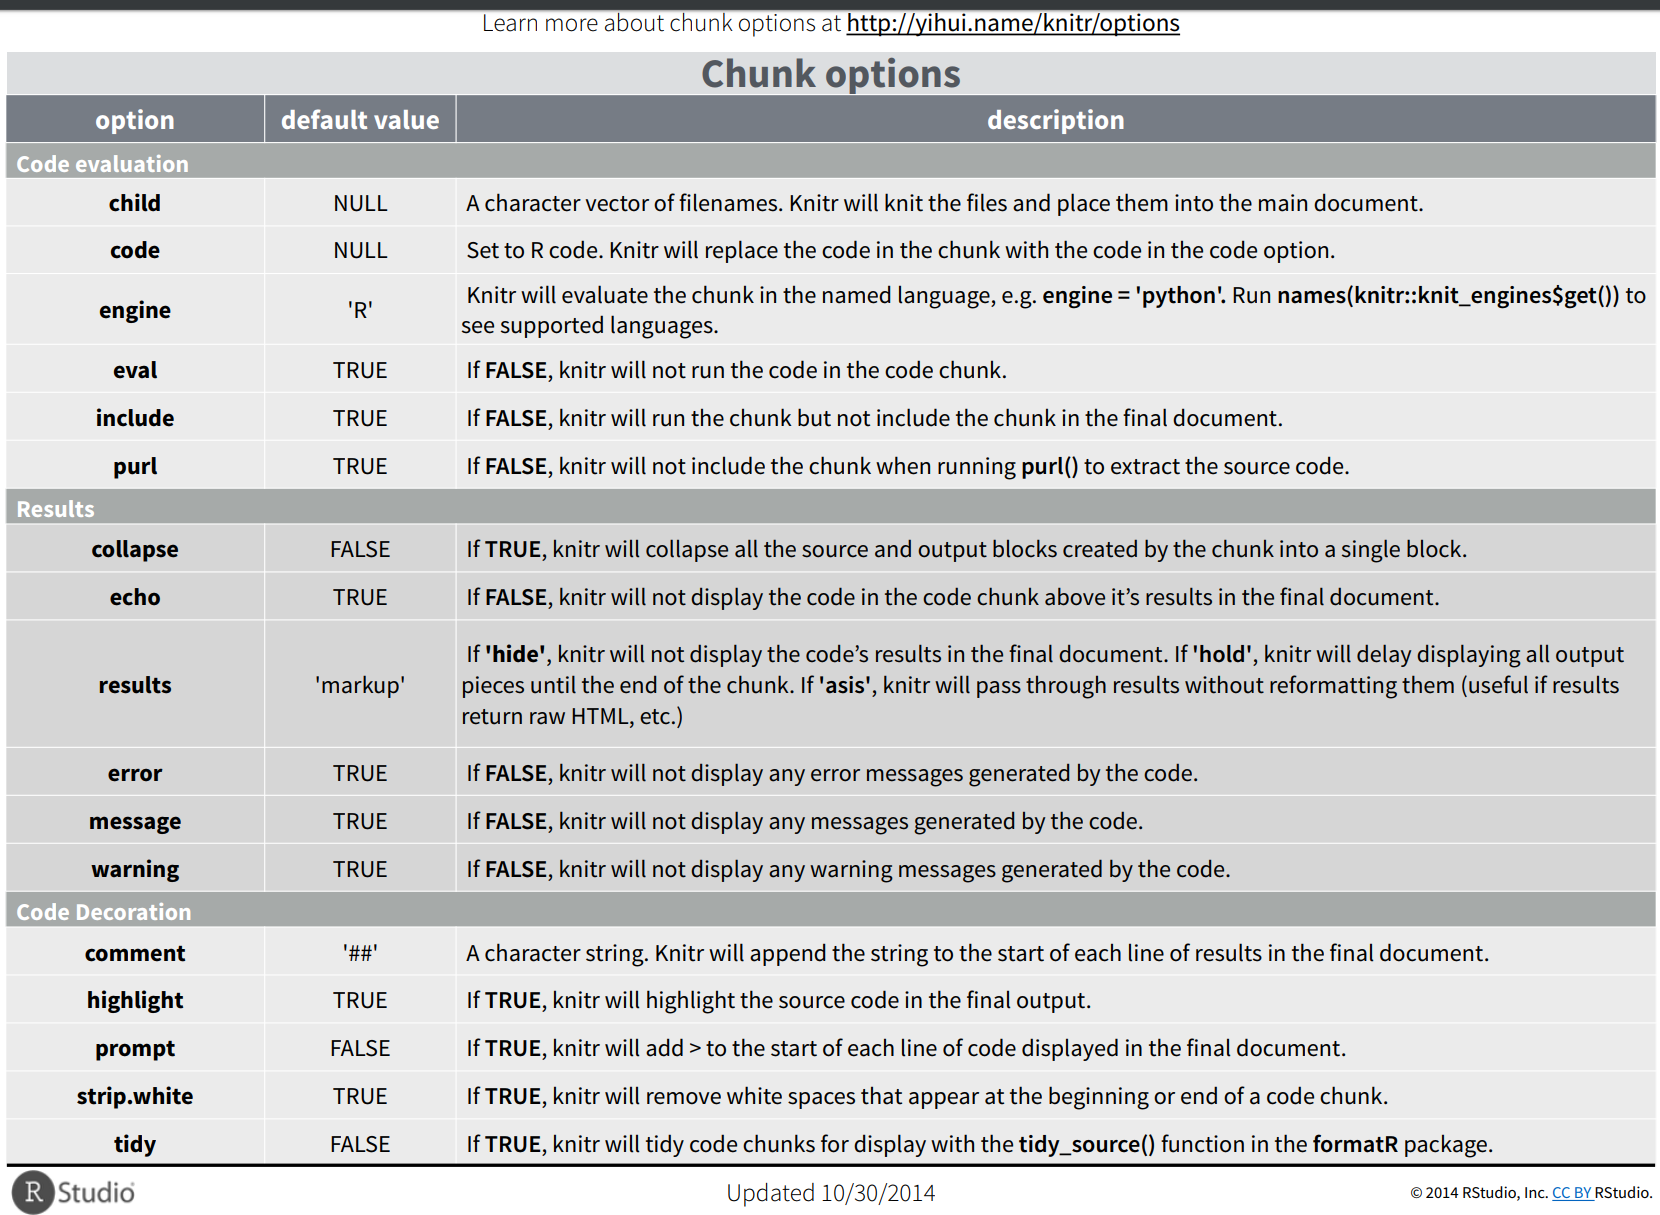
\includegraphics[width=\textwidth, keepaspectratio]{img/rr/knitropts.png}
\caption[knitr options]{A schematic table of options available using knitr and rmarkdown packages.}
\label{fig:knitropts}
\end{figure}


\subsubsection{Class Methods}

The class is provided of several methods for \textit{rmarkdown} \gls{cc} construction.

Once an \textit{easyReporting} instance is available, with \lstinline!mkdTitle! it is possible to insert six levels of titles, by setting the parameters \lstinline!title! and \lstinline!level!.
It is also possible to add natural language comments with \lstinline!mkdGeneralMsg!.

When working with \glspl{cc}, two main choices are available.
The first one gives the possibility to construct a \gls{cc} as additional steps, by using first the \lstinline!mkdCodeChunkSt!, then adding variable assignment and/or function calling with \lstinline!mkdVariableAssignment! or \lstinline!mkdGeneralMsg!, and finally closing the \gls{cc} with \lstinline!mkdCodeChunkEnd!.

In particular, when starting a \gls{cc} with \lstinline!mkdCodeChunkSt!, it is possible to assign a specific \lstinline!optionList! and/or a \lstinline!source.files.list! to be added to that \gls{cc}.

Otherwise it is possible to create an entire \gls{cc} just with \lstinline!mkdCodeChunkComplete! and assigning the entire function call as a \lstinline!message!.
This way of working is really useful with \lstinline!function! creation, where inside a developed function a simple recursive call with parameters assignment can be done as a single \lstinline!message!.





\section{Reproducible Computational Research} \label{sec:integrhorr}
The most difficult part while using a \gls{gui} is keeping track the executed functionalities during the analysis.
To face this need we equipped \gls{igro} of a \gls{rr} hidden layer (with aid of \textit{easyReporting} package) able to trace all executed code by the user.

In combination with a system of \gls{cdf}, \gls{igro} stores code chunks and the input/output data of each analysis step inside an \gls{rmd} file.

\begin{figure}
\centering
\begin{subfigure}{.5\textwidth}
  \centering
  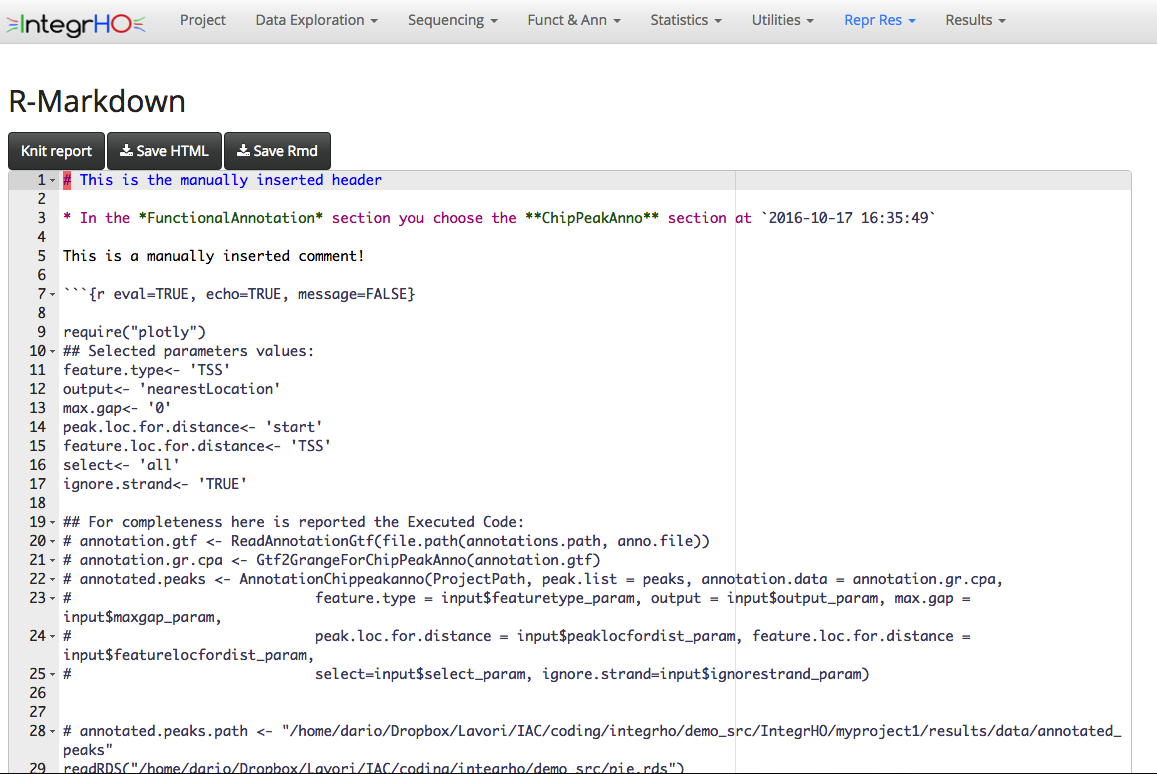
\includegraphics[width=.9\linewidth]{img/integrho/rr_1.png}
  \caption{The Interface for the editing of an auto-generated report with \gls{igro} web platform.}
  \label{fig:integrhorr1}
\end{subfigure}%
\begin{subfigure}{.5\textwidth}
  \centering
  \includegraphics[width=.9\linewidth]{img/integrho/rr_2.png}
  \caption{The report compiled and enriched with manually inserted comments throught the interface showed in the (a) panel.}
  \label{fig:integrhorr2}
\end{subfigure}
\caption[IntegrHO report editing]{The reproducible research with \gls{igro}.}
\label{fig:integrhorr}
\end{figure}

The auto-produced \gls{rmd} file as it is, it's not usable to be showed to third-parties, because it needs to be enriched with natural language comments.
To account for this need, we built a specific interface enabling the user to edit the automatically produced \gls{rmd} file and to compile it on the fly (see sub-figure \ref{fig:integrhorr1}).

The enriched output report can be produced in \gls{html} (sub-figure \ref{fig:integrhorr2}) or \gls{pdf} formats, in order to be easily attached as supplementary material of a published article, facilitating the reproducibility of the analysis to third-party users.

Furthermore, thanks to the \gls{cdf} system, each code chunk is not dependent on previous ones, enabling the final user to add/remove multiple code chunks.
\section{Discussions} \label{sec:integrhofuture}
Multiple omics data information extraction became always more complex with the evolution of sequencing techniques and with the consequent development of methodologies for their analysis and integration.
With this thesis work, we focused on the development of novel strategies for several problems related to multiple omics sequencing data information extraction.

Firstly, we approached the most studied genomic problem, transcriptomic, by focusing on time-course \textit{RNA-seq} data.
We presented \textit{ticorser}, an R command line package for time-course \textit{RNA-seq} data.
With this instrument we propose a complete pipeline for the time-course data analysis, presenting also ad-hoc designed approaches for this type of data visualization at different levels.
Additionally, allowing a first integration level with functional annotation and also for their visualization.

Afterwards, we focused on \textit{ATAC-seq} technology, an emerging technique for open chromatin region detection, which still needs appropriate solutions for its analysis.
To address the lack of methodologies with this data we presented \textit{DEScan2}, an R/Bioconductor package allowing detection of open chromatin regions, and proposed a possible workflow for the detection of \glspl{der} and their integration with \textit{RNA-seq} data.

Due to the difficulty of keeping track even a single omic analysis, we presented \textit{easyReporting}, a possible approach to the Reproducible Research inside R.
A tool which helps not only software developers to include \gls{rr} layers inside their tools, but also non-expert R analysts to easily produce reports for their analysis.

Finally, to speed up and help also non-expert users to analyze multiple omics data, we presented \gls{igro}, a web graphical user interface for the analysis of omics data.
Combining the flexibility of a point-and-click approach with the power of R/Bioconductor statistical approaches for the omics data analysis.
Moreover, thanks to the Reproducible Research layer it allows to keep track of all the steps performed during the analysis, and with aid of dedicated interface to live edit the enriched report.

%\chapter{Conclusions \& Future Works} \label{sec:integrhofuture}
%Multiple omics data information extraction became always more complex with the evolution of sequencing techniques and with the consequent development of methodologies for their analysis and integration.
With this thesis work, we focused on the development of novel strategies for several problems related to multiple omics sequencing data information extraction.

Firstly, we approached the most studied genomic problem, transcriptomic, by focusing on time-course \textit{RNA-seq} data.
We presented \textit{ticorser}, an R command line package for time-course \textit{RNA-seq} data.
With this instrument we propose a complete pipeline for the time-course data analysis, presenting also ad-hoc designed approaches for this type of data visualization at different levels.
Additionally, allowing a first integration level with functional annotation and also for their visualization.

Afterwards, we focused on \textit{ATAC-seq} technology, an emerging technique for open chromatin region detection, which still needs appropriate solutions for its analysis.
To address the lack of methodologies with this data we presented \textit{DEScan2}, an R/Bioconductor package allowing detection of open chromatin regions, and proposed a possible workflow for the detection of \glspl{der} and their integration with \textit{RNA-seq} data.

Due to the difficulty of keeping track even a single omic analysis, we presented \textit{easyReporting}, a possible approach to the Reproducible Research inside R.
A tool which helps not only software developers to include \gls{rr} layers inside their tools, but also non-expert R analysts to easily produce reports for their analysis.

Finally, to speed up and help also non-expert users to analyze multiple omics data, we presented \gls{igro}, a web graphical user interface for the analysis of omics data.
Combining the flexibility of a point-and-click approach with the power of R/Bioconductor statistical approaches for the omics data analysis.
Moreover, thanks to the Reproducible Research layer it allows to keep track of all the steps performed during the analysis, and with aid of dedicated interface to live edit the enriched report.
%\subsection{Single Omic Approach}  \label{sec:integrhosingleomic}
%\input{sections/integrho/singleomic.tex}
%\subsection{Multi Omic Approach}  \label{sec:integrhomultiomic}
%\input{sections/integrho/multiomic.tex}
%\subsubsection{Low Level Itegration} \label{sec:integrholowlev}
%\input{sections/integrho/lowlev.tex}
%\subsubsection{High Level Itegration} \label{sec:integrhohighlev}
%\input{sections/integrho/highlev.tex}
%\section{Implementation Aspects} \label{sec:integrhoimpl}
%\gls{igro} is a web based \gls{gui} for the analysis and the integration of multiple \gls{ngs} data with the aid of several already published packages designed for this aim. 

For the \gls{gui} implementation we used the R \textit{Shiny} libraries because of its power to render R code in web format.

The tool presents itself with a main upper menu of main topics organized by scope. For each of this topic, a sub-menu with specific functionalities is available.
Moreover, depending on the selected functionality, a side menu is presented with additional functionalities or with input parameters to setup the specific tool.
After the parameter setup the results in graphical or table format are presented in the main part of the interface. (figure \ref{fig:integrhomain})

Before to proceed to its data analysis, it is mandatory for the user to setup the project with a dedicated interface. 
The user has to upload a design matrix which describes the information related to its samples, some of them are mandatory as the filename (with path) of the BAM files and the condition of each sample, while others are optional as the tissue or the run id. It is also possible to edit the design matrix by hand directly from the interface.
In such a way \gls{igro} creates in the working directory (returned by the \lstinline!getwd()! function) a dedicated folder with all the required subfolders and stores all the basic information of the project into an ad-hoc designed \lstinline!R6ProjectClass! which will be re-used during the whole session to speed up the configuration of each step of the analysis.

\begin{figure}[H]
\includegraphics[width=\textwidth, keepaspectratio]{img/integrho/general_description.png}
\caption[integrho main interface]{}
\label{fig:integrhomain}
\centering
\end{figure}
 
\gls{igro} implements several functionalities and methodologies for \textit{RNA-Seq}, \textit{ChIP-Seq} and \textit{ATAC-Seq} data analysis, complementing these aspects by providing methodologies for their integration at different levels, as functional enrichment with Gene Ontology and Pathways,  peaks and genes annotation, and more statistical methods, as mixOmics, working with high-dimensional datasets.

For each -omics, \gls{igro} takes as input the BAM files, previously defined in the design matrix of the main project definition interface.

For each step of the analysis of each -omics, we tried to select more than one method to perform that task. 
In so doing we give the possibility to try different approaches in order to compare the final results, tuning the methods on the basis of the dataset under investigation.

For \textit{RNA-Seq} we constructed a dedicated interface for each step of a standard RNA-Seq data analysis pipeline, such as to build a count matrix, to filter out low counts with multiple tests, to normalize them and to account for batch effect. 
Moreover, we selected multiple methods for \gls{deg}, such as \textit{edgeR}, \textit{DESeq2}, \textit{NOISeq}.

For \textit{ChIP-Seq} we constructed specific interfaces for peak calling, annotation and \glspl{der} detection.
For the peak calling, because of the lack of specific methods starting from BAM files, we implemented interfaces for the DEScan2 and the \textit{csaw}\cite{Lun2015} peak callers. The first one born for broad peaks identification and the second one for both broad and narrow peaks quantification.
For the annotation we chose the \textit{ChIPpeakAnno} and the \textit{ChIPseeker} R/Bioconductor, which produces similar output formats starting from peaks. While for the detection of \glspl{der} we used the same methods as for \textit{RNA-Seq}.

For \textit{ATAC-Seq} we used mostly the same methods implemented for the \textit{ChIP-Seq}, but designing specific interfaces for the filtering/alignment and the counting matrix as implemented in the DEScan2 package (see chapter \ref{sec:descan2cap} for further details).

To provide an integration of these -omics, we dedicated an entire section to this aspect, with functionalities for the annotation of \glspl{der} with \glspl{deg} using \textit{ChIPpeakAnno} and to use this information to investigate the functional response by enriching for Gene Ontology or for Pathways.
These last two aspects implemented with aid of \textit{g:Profiler} \cite{Reimand2016} and \textit{graphite} \cite{Sales2012a} R/Bioconductor packages.

Moreover, to work with high-dimentional data sets, we are working on the implementation of methods like mixOmics, which gives a graphical response of the samples or the features, using two different methods diablo and mint.

%\section{Results} \label{sec:integrhoresults}
%\textbf{Few words on ATAC-Seq data}

We illustrate the performances of \gls{descan} using a dataset \cite{Su2017} that describes in vivo adult mouse dentate granule neurons before and after synchronous neuronal activation using Atac-Seq and RNA-Seq technologies (see sections \ref{sec:atacseq} and \ref{sec:rnaseq} for a description of these sequencing techniques).

This dataset is organized in 62 samples of Atac-Seq and RNA-Seq, extracted at different time points, with four replicates at each time point.
We chose to compare the differences btween the first two stages, time 0 (E0) and 1 hour after neuronal induction (E1), in order to show a possible Atac-Sec workflow for Differential Enrichment, and how to integrate this data type with RNA-Seq. A general illustration of our dataset is represented in figure \ref{fig:atacdataset}.

\begin{figure}[H]
\includegraphics[width=\textwidth,height=\textheight,keepaspectratio]{img/descan2/dataset.png}
\caption[DEScan2 dataset illustration]{An illustration of our extraction of the \cite{Su2017} dataset.}
\label{fig:atacdataset}
\centering
\end{figure}

We downloaded the data from \gls{geo} database \cite{Edgar2002, Barrett2013} with accession number GSE82015\footnote{\url{https://www.ncbi.nlm.nih.gov/geo/query/acc.cgi?acc=GSE82015}} and mapped raw data using \textit{STAR} \cite{Dobin2013} with default parameter on \gls{mm10}.

In order to detect the open chromatin regions we run our peak caller, cutting the genome in bins of 50bp and using running windows of minimum 50bp and maximum 1000bp. In such a way we are able to detect not just broad peak, but also smaller peaks.

To be confident with our results we compared the \gls{descan} detected peaks with the same validated regions (Arc and Gabrr1) in the original work \cite{Su2017}.
The lower part of figure \ref{fig:peaksdescan} shows the detected and validated regions (in blue and red) resulting differentially enriched between the E0 (in pink) and E1 (in green) conditions, while the upper part shows \gls{descan} peaks (in blue), highlighting a capability to catch not only the same regions of the published ones, but also (gold circles) to be more careful in the smaller peaks detection.

\begin{figure}[H]
\includegraphics[width=\textwidth,height=\textheight,keepaspectratio]{img/descan2/peaks.png}
\caption[\gls{descan} peaks detection]{A comparison of \gls{descan} detected peaks with validated peaks in article \cite{Su2017}.}
\label{fig:peaksdescan}
\centering
\end{figure}

Moreover, we run \textit{MACS2} on the same samples, and (as shown in figure \ref{fig:des2m2peaks}) \gls{descan} seems able to catch much more peaks than \textit{MACS2} for each sample.

\begin{figure}[H]
\includegraphics[width=\textwidth,height=\textheight,keepaspectratio]{img/descan2/d2m2_peaks_number.png}
\caption[The \gls{descan} and \textit{MACS2} peaks detection]{A comparison of \gls{descan} and \textit{MACS2} detected peaks for each sample in the dataset.}
\label{fig:des2m2peaks}
\centering
\end{figure}

While it is very important to detect good peaks with a peak caller, it seems to be more relevant to detect reliable regions. Indeed, during the filtering step, the number of peaks depends not only by the peak score, but also by the number of replicates designed in the experiment.
The figure \ref{fig:filteringdescan} puts in relation these two relevant information. 
On the x-axis is represented the number of replicates, while on the y-axis is traced the number of peaks, and each curve represents a different threshold on the peaks score, showing that higher are the thresholds on the scores and the number of replicates, lower is the number of the detected peaks.
Highlighting a proportional inversion between the number of the peaks and the combination of the number of samples and the detected regions score.


\begin{figure}[H]
\includegraphics[width=\textwidth, height=\textheight, keepaspectratio]{img/descan2/filtering.png}
\caption[\gls{descan} filtering step]{Filtering the detected regions with different thresholds on peak scores.}
\label{fig:filteringdescan}
\centering
\end{figure}


\begin{figure}[H]
\includegraphics[width=\textwidth, height=\textheight, keepaspectratio]{img/descan2/filtering_m2_d2.png}
\caption[\gls{descan} and \textit{MACS2} filtering comparison]{Filtering the detected regions with different thresholds on peak scores between \textit{MACS2} and \gls{descan}.}
\label{fig:filteringdescanmacs2}
\centering
\end{figure}

The filtered-in regions can be processed by \gls{descan} in order to obtain a count matrix with samples on the columns and peaks on the rows.
This type of data structure is very versatile, because it enables to perform several operations, like the \glspl{der} and, if possible, the integration with other kind of omics, as RNA-Seq.

In order to preserve the information associated to the peaks, \gls{descan} produces as output a \textit{SummarizedExperiment} (figure \ref{fig:countsdescan}) data structure, which enables to retrieve the count matrix with \lstinline{assays} method, and to access the peaks information in \textit{GenomicRanges} format with the \lstinline{rowRanges} method. %{

\begin{figure}[H]
\centering
\includegraphics[keepaspectratio]{img/descan2/counts.png}
\caption[\gls{descan} counts illustration]{An illustration of the \textit{SummarizedExperiment} data structure produced by \gls{descan}.}
\label{fig:countsdescan}
\centering
\end{figure}

Before to proceed to detect \glspl{der}, it is a good standard to normalize the data, also because without any kind of normalization we are not able to detect any \gls{der}.
The nature of the data, in count format, makes it possible to apply several well known RNA-Seq normalizations techniques, as \textit{TMM}, \textit{upper-quartile}, \textit{full-quantile}, \textit{RUV-Seq}, etc \cite{Risso2014, Robinson2010, Dillies2013}.

While the \textit{TMM} and \textit{upper-quartile} normalizations modify the data in a way that makes it impossible to detect \glspl{der}, other kind of normalizations and combinantions of them give good results.

The figure \ref{fig:normalizationsdescan} sintetizes this concept very well, highlighting a relation between the number of \glspl{der} and the minumum number of samples used for filtering the data during the \gls{descan} filtering step.

The plot shows that \textit{upper-quantile}, even if combined with \textit{RUV-Seq} normalization, is not able to linearly detect a good amount of \glspl{der}, while \textit{full-quantile}, when combined with \textit{RUV-Seq} seems to affect the data in a way that overdetect the number of \glspl{der}. 
When looking at the \textit{full-quantile} and \textit{RUV-Seq} by themself seem to perform better than the other normalizations. The first one has a downhill almost linear, while the second one has a very fast downhill with a regrowth when the number of samples is higher.

Even if these normalization methods show good performances with this type of epignomic data, our investigations suggest that more testing is required, but maybe an ad-hoc normalization method for these data has to be developed.

\begin{figure}[H]
\centering
\includegraphics[width=\textwidth, height=\textheight, keepaspectratio]{img/descan2/normalizations.png}
\caption[Normalizations applied to detected regions]{The figure shows the effects of different normalizations on the epigenomic differentially enriched regions.}
\label{fig:normalizationsdescan}
\centering
\end{figure}

To estimate the \glspl{der}, any of the RNA-Seq methods can be applied, such as \textit{DESeq2}, \textit{edgeR}, \textit{NOISeq}, etc \cite{Robinson2009, McCarthy2012, Tarazona2012}.

In this case, we decided to use \textit{edgeR} package, because of its wide range of  available statistical approaches and the possibility to better tune the design of the experiment. 
Indeed, because we used the RUV-Seq normalized counts with \lstinline{k} parameter set to 4, we modeled the experimental design with the \lstinline{model.matrix} function, adding to our model not only the experimental conditions, but also the RUV-Seq estimated weights.
Then we used the resulted design to estimate the dispersion and fit a Quasi-Likelihood test, as defined in edgeR.

The figure \ref{fig:depeaksdescan} shows a volcano plot of \glspl{der} between E0 and E1 conditions.
Red dots highlights the regions with a False Discovery Rate (FDR) lower than 0.05, while blue dots highlight not significant regions.
 
\begin{figure}[h]
\centering
\includegraphics[width=\textwidth, height=\textheight, keepaspectratio]{img/descan2/DE_peaks.png}
\caption[Differential Enrichment Regions Volcano]{A volcano plot of Differential Enriched Regions. Blue dots represent the not significant \glspl{der}, while the red ones represent the significant \glspl{der}.}
\label{fig:depeaksdescan}
\centering
\end{figure}

Next task is to integrate the obtained results with other omic data types, as RNA-Seq. 
Because of the low number of the samples, the easiest way to integrate the data is to annotate the \glspl{der} with differentially expressed genes resulting from the analysis of RNA-Seq.

For the Differential expression of the RNA-Seq data we firstly quantified the signal with \lstinline{featureCounts} methods available in the \textit{Rsubread} \cite{Liao2013} Bioconductor package.
Then we filtered lowly expressed genes with the \textit{proportion} test  as implemented in \textit{NOISeq} package, and applied the \lstinline{noiseq} method for differential expression.%{

\begin{figure}[h]
\centering
\includegraphics[width=\textwidth, height=\textheight, keepaspectratio]{img/descan2/Annotated_depeaks_degenes.png}
\caption[Annotated Differential Enrichment Regions Volcano]{A volcano plot of \glspl{der}. Blue dots represent the not significant \glspl{der}, while the red ones represent the significant \glspl{der}. Green circles highlights the peaks with a \gls{deg} annotated.}
\label{fig:depeakdegenessdescan}
\centering
\end{figure}

We selected the significant \glspl{deg} with a probability higher than 0.95, and used these genes to annotate the peaks with \lstinline{annotatePeakInBatch} method of ChIPpeakAnno.
Figure 	\ref{fig:depeakdegenessdescan} illustrates with green circles the peaks with an annotated gene with distance lower than 10000bp from the gene TSS.
Realizing the plot with the \textit{plotly} library it's possible to enhance the names of the genes with a tip window.











%%%%%%%%%%%%%%%%%%%%%%%%%%%%%%%%%%%%%%%%%%%%%%%%%%%%%%%%%%%%%
\chapter{Conclusions}
Multiple omics data information extraction became always more complex with the evolution of sequencing techniques and with the consequent development of methodologies for their analysis and integration.
With this thesis work, we focused on the development of novel strategies for several problems related to multiple omics sequencing data information extraction.

Firstly, we approached the most studied genomic problem, transcriptomic, by focusing on time-course \textit{RNA-seq} data.
We presented \textit{ticorser}, an R command line package for time-course \textit{RNA-seq} data.
With this instrument we propose a complete pipeline for the time-course data analysis, presenting also ad-hoc designed approaches for this type of data visualization at different levels.
Additionally, allowing a first integration level with functional annotation and also for their visualization.

Afterwards, we focused on \textit{ATAC-seq} technology, an emerging technique for open chromatin region detection, which still needs appropriate solutions for its analysis.
To address the lack of methodologies with this data we presented \textit{DEScan2}, an R/Bioconductor package allowing detection of open chromatin regions, and proposed a possible workflow for the detection of \glspl{der} and their integration with \textit{RNA-seq} data.

Due to the difficulty of keeping track even a single omic analysis, we presented \textit{easyReporting}, a possible approach to the Reproducible Research inside R.
A tool which helps not only software developers to include \gls{rr} layers inside their tools, but also non-expert R analysts to easily produce reports for their analysis.

Finally, to speed up and help also non-expert users to analyze multiple omics data, we presented \gls{igro}, a web graphical user interface for the analysis of omics data.
Combining the flexibility of a point-and-click approach with the power of R/Bioconductor statistical approaches for the omics data analysis.
Moreover, thanks to the Reproducible Research layer it allows to keep track of all the steps performed during the analysis, and with aid of dedicated interface to live edit the enriched report.

%\begin{appendices}
%\section{R Language} \label{sec:rlang}
%\section{R Markdown Language} \label{sec:rmarkdown}
%\end{appendices}



\printbibliography[heading=bibnumbered]
\cleardoublepage

%\printglossaries
%
%\cleardoublepage
% \phantomsection
\addcontentsline{toc}{chapter}{\listfigurename}
\listoffigures

\cleardoublepage
% \phantomsection
%\addcontentsline{toc}{chapter}{\listtablename}
%\listoftables

%\listoffigures
%\listoftables

\end{document}